% ===========================================================================
%  EGH490-2 Project Delivery Report -- Jared Saunders (n11034459)
%  Controlling Differential Power Processors in Solar Powered Applications
%
%  Open in Overleaf: upload the whole folder (zip), set the compiler to
%  pdfLaTeX, main document = main.tex.  Bibliography: refs.bib (bibtex,
%  IEEEtran style; falls back to ieeetr if IEEEtran.bst is missing).
%
%  Authoring conventions (see README.md):
%    talking   environment  -> purple bullets: points to turn into prose
%    \note{..}              -> orange: a decision for you / something to confirm
%    \ev{..}                -> plain text (evidence colouring removed)
%  Put \tpoff in this file to print talking points in black, \tphide to drop
%  them from the PDF (e.g. for the submitted version).
% ===========================================================================
\documentclass[12pt,a4paper]{article}
% ---------------------------------------------------------------------------
% Preamble: EGH490-2 Project Delivery Report (A4, 12 pt, 20 mm margins)
% Compiles with pdflatex + bibtex on Overleaf (TeX Live 2024) and locally.
% ---------------------------------------------------------------------------
\usepackage[utf8]{inputenc}
\usepackage[T1]{fontenc}
\usepackage{mathptmx}                 % Times text + maths (12 pt body as required)
\usepackage[scaled=0.92]{helvet}      % Arial-like sans for headings / tables
\usepackage[a4paper,top=20mm,bottom=20mm,left=20mm,right=20mm,headheight=14pt]{geometry}
\usepackage{amsmath,amssymb,bm}
\usepackage{graphicx}
\graphicspath{{figures/}{figures/slides/}{figures/pipeline/}{figures/photos/}{figures/sim/}{figures/misc/}{figures/tikz/}}
\usepackage[table]{xcolor}
\usepackage{booktabs,longtable,array,multirow,makecell,tabularx,colortbl}
\usepackage{caption,subcaption}
\captionsetup{font=small,labelfont=bf,width=0.95\linewidth}
\setlength{\textfloatsep}{10pt plus 2pt minus 4pt}
\setlength{\floatsep}{8pt plus 2pt minus 2pt}
\setlength{\intextsep}{8pt plus 2pt minus 2pt}
\renewcommand{\topfraction}{0.85}
\renewcommand{\bottomfraction}{0.6}
\renewcommand{\textfraction}{0.1}
\renewcommand{\floatpagefraction}{0.8}
\setcounter{topnumber}{3}
\setcounter{totalnumber}{5}
\usepackage{float,placeins}
\usepackage{enumitem}
\setlist{nosep,leftmargin=*}
\usepackage{fancyhdr}
\usepackage{titlesec}
\usepackage{pdflscape}
\usepackage{listings}
\usepackage{tikz}
\usetikzlibrary{arrows.meta,positioning,shapes.geometric,calc,fit,backgrounds,chains,decorations.pathreplacing}
\usepackage{circuitikz}
\usepackage{microtype}
\usepackage{xspace}
\usepackage{csquotes}
\usepackage[colorlinks=true,linkcolor=blue!50!black,citecolor=blue!50!black,urlcolor=blue!50!black]{hyperref}
\usepackage{cleveref}

% ----- headings in sans, numbered to subsubsection
\titleformat{\section}{\sffamily\Large\bfseries}{\thesection}{0.8em}{}
\titleformat{\subsection}{\sffamily\large\bfseries}{\thesubsection}{0.8em}{}
\titleformat{\subsubsection}{\sffamily\normalsize\bfseries}{\thesubsubsection}{0.8em}{}
\titlespacing*{\section}{0pt}{14pt}{6pt}
\titlespacing*{\subsection}{0pt}{10pt}{4pt}
\setcounter{secnumdepth}{3}
\setcounter{tocdepth}{2}

% ----- header / footer
\pagestyle{fancy}
\fancyhf{}
\fancyhead[L]{\small\sffamily Controlling Differential Power Processors in Solar Powered Applications}
\fancyhead[R]{\small\sffamily Jared Saunders \textperiodcentered{} n11034459}
\fancyfoot[C]{\small\sffamily Page \thepage}
\renewcommand{\headrulewidth}{0.3pt}

% ----- colours
\definecolor{tpcol}{RGB}{120,90,170}      % talking points
\definecolor{notecol}{RGB}{190,80,30}     % notes to self / to decide
\definecolor{evcol}{RGB}{30,110,70}       % evidence callouts
\definecolor{anacol}{RGB}{107,107,107}
\definecolor{milcol}{RGB}{142,107,191}
\definecolor{simcol}{RGB}{31,107,70}
\definecolor{qspcol}{RGB}{27,45,85}
\definecolor{hwcol}{RGB}{217,130,43}

% ----- authoring helpers -------------------------------------------------
% Talking points: bullets you still have to turn into prose. Printed in
% colour so they are easy to find; set \tpoff to print them in black, or
% \tphide to drop them from the PDF entirely.
\newif\iftpshow \tpshowtrue
\newcommand{\tpoff}{\colorlet{tpcol}{black}}
\newcommand{\tphide}{\tpshowfalse}
\newenvironment{talking}{\iftpshow\begin{itemize}[label=\textcolor{tpcol}{$\triangleright$},leftmargin=1.4em]\color{tpcol}\small\else\setbox0\vbox\bgroup\fi}{\iftpshow\end{itemize}\else\egroup\fi}
% Short orange note for decisions / things to confirm.
\newcommand{\note}[1]{\iftpshow{\color{notecol}\small\textbf{[note]} #1}\fi}
% Evidence callout (a number taken from the pipeline tables, with its source).
\newcommand{\ev}[1]{#1}
% Units and symbols
\newcommand{\unit}[1]{\ensuremath{\,\mathrm{#1}}}
\newcommand{\us}{\unit{\mu s}}
\newcommand{\ms}{\unit{ms}}
\newcommand{\kHz}{\unit{kHz}}
\newcommand{\V}{\unit{V}}
\newcommand{\A}{\unit{A}}
\newcommand{\W}{\unit{W}}
\newcommand{\Wh}{\unit{Wh}}
\newcommand{\ohm}{\ensuremath{\,\Omega}}
\newcommand{\uH}{\ensuremath{\,\mu\mathrm{H}}}
\newcommand{\uF}{\ensuremath{\,\mu\mathrm{F}}}
\newcommand{\Vbar}{\ensuremath{\bar{V}}}
\newcommand{\vd}{\ensuremath{v_{d}}}
\newcommand{\ic}{\ensuremath{i_{c}}}
\newcommand{\im}{\ensuremath{i_{m}}}
\newcommand{\uc}{\ensuremath{u_{c}}}
\newcommand{\ud}{\ensuremath{u_{d}}}
\newcommand{\fsw}{\ensuremath{f_{sw}}}
\newcommand{\kscale}{k}
\newcommand{\code}[1]{\texttt{#1}}

% ----- pseudocode via listings (works everywhere, no algorithm2e needed)
\definecolor{qutnavy}{RGB}{0,64,122}
\definecolor{codebg}{RGB}{246,248,251}
\definecolor{codecomment}{RGB}{110,118,129}
\lstdefinelanguage{pseudo}{
  morekeywords={if,else,elif,for,each,while,return,every,then,and,or,not,in,do,end,function,on,switch,case,down,to},
  morekeywords=[2]{trip,clamp,max,min,ramp},
  sensitive=true, morecomment=[l]{\#}, morestring=[b]"}
\lstset{language=pseudo,basicstyle=\fontfamily{lmtt}\selectfont\footnotesize,
  keywordstyle=\color{qutnavy}\bfseries,keywordstyle=[2]\color{qutnavy},
  commentstyle=\color{codecomment},stringstyle=\color{qutnavy},
  columns=fixed,basewidth=0.52em,keepspaces=true,breaklines=true,breakindent=4em,
  postbreak=\mbox{\textcolor{codecomment}{$\hookrightarrow$}\space},
  frame=tb,framerule=0.6pt,rulecolor=\color{qutnavy},backgroundcolor=\color{codebg},
  framexleftmargin=4pt,framexrightmargin=4pt,xleftmargin=4pt,xrightmargin=4pt,
  aboveskip=8pt,belowskip=8pt,captionpos=t,numbers=none,tabsize=4}
\renewcommand{\lstlistingname}{Listing}

% ----- tikz styles for the diagrams
\tikzset{
  blk/.style={draw,rounded corners=2pt,fill=white,minimum height=8mm,minimum width=22mm,align=center,font=\sffamily\small},
  blkb/.style={blk,fill=blue!6},
  blkg/.style={blk,fill=green!8},
  blko/.style={blk,fill=orange!10},
  blkr/.style={blk,fill=red!8},
  blky/.style={blk,fill=yellow!15},
  arr/.style={-{Stealth[length=2mm]},thick},
  darr/.style={{Stealth[length=2mm]}-{Stealth[length=2mm]},thick},
  lab/.style={font=\sffamily\scriptsize,fill=white,inner sep=1pt},
  st/.style={draw,ellipse,fill=blue!6,minimum width=18mm,minimum height=7mm,font=\sffamily\small,align=center},
  stf/.style={st,fill=red!12},
}

\tphide

\begin{document}

\pagenumbering{alph}% unique anchor for the title page (avoids a duplicate page.1)
% Title page in the style of the proposal / progress report: navy QUT banner
% with the logo, blue title block, tinted people panel and version table.
\definecolor{qutnavy}{RGB}{0,64,122}
\definecolor{qutblue}{RGB}{15,82,150}
\definecolor{qutpale}{RGB}{244,247,251}
\definecolor{qutfoot}{RGB}{226,231,238}
\begin{titlepage}
\thispagestyle{empty}
\sffamily
\begin{tikzpicture}[remember picture,overlay]
  % banner
  \fill[qutnavy] (current page.north west) rectangle ([yshift=-38mm]current page.north east);
  \node[anchor=north east,inner sep=0pt] at ([xshift=-20mm,yshift=-6mm]current page.north east)
       {
\includegraphics[height=26mm]{misc/qut_logo}};
  \draw[white,line width=0.6pt] ([xshift=-20mm,yshift=-6mm]current page.north east) rectangle ++(-26mm,-26mm);
  \node[anchor=west,text=white,align=left] at ([xshift=20mm,yshift=-16mm]current page.north west)
       {\large\bfseries QUEENSLAND UNIVERSITY OF TECHNOLOGY\\[3pt]\normalsize\color{white!80!qutnavy}EGH490-2 \textperiodcentered{} Research Project 2};
  % footer band
  \fill[qutfoot] (current page.south west) rectangle ([yshift=16mm]current page.south east);
  \fill[qutnavy] (current page.south west) rectangle ([yshift=2.2mm]current page.south east);
  \node[anchor=west,text=qutnavy!70] at ([xshift=20mm,yshift=9mm]current page.south west) {\small October 23, 2026};
  \node[anchor=east,text=qutnavy!70] at ([xshift=-20mm,yshift=9mm]current page.south east) {\small Jared Saunders \textperiodcentered{} n11034459};
\end{tikzpicture}

\vspace*{22mm}
\begin{center}
{\color{qutnavy!75}\large PROJECT DELIVERY REPORT}

\vspace{9mm}
{\color{qutblue}\fontsize{25}{31}\selectfont\bfseries Controlling Differential Power Processors\\[2pt] in Solar Powered Applications\par}

\vspace{7mm}
{\color{qutblue}\rule{22mm}{1.2pt}}

\vspace{7mm}
{\color{qutnavy!80}\large THE DESIGN AND IMPLEMENTATION OF MODERN STATE-SPACE\\[2pt] METHODS TO SERIAL PARTIAL POWER CONVERTERS\par}

\vspace{6mm}
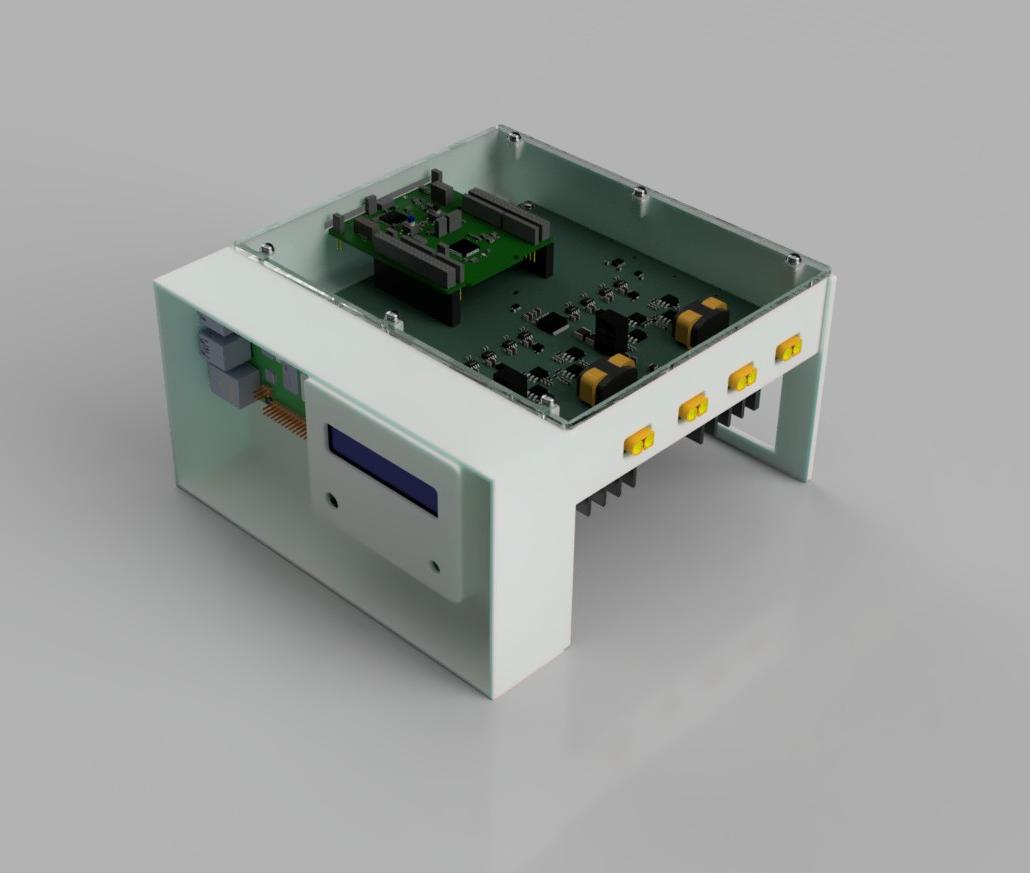
\includegraphics[height=62mm]{img-001-000}

\vspace{6mm}
\colorbox{qutpale}{\begin{minipage}{0.92\linewidth}\vspace{4mm}\centering
\begin{tabular}{p{0.38\linewidth}p{0.56\linewidth}}
\centering{\color{qutnavy}\footnotesize\bfseries STUDENT ENGINEER} & \centering{\color{qutnavy}\footnotesize\bfseries SUPERVISOR}\tabularnewline[3pt]
\centering\large Jared Saunders & \centering\large Assoc Prof Geoff Walker\tabularnewline[1pt]
\centering{\color{qutblue}\small n11034459} & \centering{\color{qutblue}\small School of Electrical Engineering \& Robotics}\tabularnewline
\end{tabular}\vspace{4mm}\end{minipage}}

\vspace{7mm}
{\small\renewcommand{\arraystretch}{1.35}%
\begin{tabular}{>{\columncolor{qutpale}}p{14mm}>{\columncolor{qutpale}}p{20mm}>{\columncolor{qutpale}}p{30mm}>{\columncolor{qutpale}}p{58mm}}
\rowcolor{qutnavy}\color{white}\scriptsize\bfseries Version & \color{white}\scriptsize\bfseries Date & \color{white}\scriptsize\bfseries Author & \color{white}\scriptsize\bfseries Changes / Comments\\
1.0 & 17/04/26 & Jared Saunders & Project Proposal\\
2.0 & 29/05/26 & Jared Saunders & Semester 1 Progress Report\\
3.0 & 23/10/26 & Jared Saunders & Project Delivery Report\\
\end{tabular}}
\end{center}
\end{titlepage}


% front matter: roman page numbers, unnumbered sections listed in the contents
\pagenumbering{roman}
\section*{Executive Summary}
\phantomsection\addcontentsline{toc}{section}{Executive Summary}
\label{sec:exec}

% ---- Condensed rework of your draft (your version: 01_executive_summary_draft.tex).
% ---- Green numbers are from the results pipeline tables.

This project designed, built and field-tested a controller for the `Power Shuffler', and showed on a real solar string that it recovers power a shaded string would otherwise lose. Shading one panel in a series string limits the current of the whole string, and the bypass diodes used to protect it simply discard the shaded panel's power. The shuffler is a serial partial power converter (S-PPC), a type of differential power processor, that instead moves the difference in power between series-connected modules to balance their voltages. A sister report covers the shuffler hardware; this report covers its control system, from the analytical model through to closed-loop validation on the bench and in the field.

Each shuffler is an interleaved buck-boost converter built from decoupling capacitors, a coupled inductor and two half-bridges. Each shuffler shares PV modules with its neighbours, so their dynamics are coupled and cannot be described by a set of single-input single-output transfer functions. The controller is therefore built on a multiple-input multiple-output state-space model with three states per shuffler (module-voltage difference, shuffled current and circulating current) and two inputs: common-mode duty (set by the two half-bridge duties together, which shuffles power between modules) and differential duty (their difference, which controls the circulating current). The development process followed a unique spin on a systems engineering approach. The analytical model set the controller architecture. A Simulink model of a four-module string validated these control loops, and its requirements drove the choice of sensors and microcontroller. The same C control core was then implemented inside a hardware-accurate QSPICE model, adding sensor noise and sampling delay, before going into the firmware unchanged. The final product is a single board with two shufflers, Hall-effect current sensors, power-monitor voltage sensors and an STM32G474RE microcontroller, housed in a 3D-printed enclosure with a Raspberry Pi 4B that streams telemetry to a timeseries database.

On the bench (NGE103 supply, DL3021 electronic load) the closed loop held the module-voltage differences within $\pm0.010\V$ and the circulating current within $\pm0.07\A$ across 22 settled test segments at 200--400\,kHz. The 44\,Hz telemetry is too slow to resolve the step response on hardware, so it is taken from the simulation models. For a 1\,V step at 30\,\% gain and 200\,kHz, QSPICE gives a rise time of 6.5\ms{} and a 2\,\% settling time of 11.9\ms{} with no overshoot, corroborated by the analytical model (7.6\ms{} and 13.6\ms). Of the switching frequencies tested, 300\,kHz was the best compromise; 400\,kHz gave marginal gains at higher losses with almost no change in response from gain increases.

The most significant result is from the solar test: three 80\,W panels without bypass diodes in series into a 61\,V constant-voltage load. With the top module shaded to almost zero current (a shirt over about a third of the panel), a plain series string would have delivered no power at all. With the shufflers running, the string delivered up to 99\W{} during the shading event and 10.6\Wh{} over 36 minutes of testing, nearly all of it energy that would otherwise have been lost.

The main limitation is scope: one board with two shufflers that are hard-wired together, so they cannot be driven independently and boards cannot be stacked, which leaves scalability untested. The top-level INA239 (U10) does not work, so $V_{M1}$ was inferred from the electronic load; the gains have to be re-derived in simulation whenever the switching frequency changes; and poor weather on the test day meant the closed loop was only partly exercised against real panel dynamics. The recommended next steps are a stackable board with independently driven shufflers, to test strings of more than three modules, and a study of other applications for S-PPCs that may offer more impact to industry than solar.

\clearpage
\section*{Abstract}
\phantomsection\addcontentsline{toc}{section}{Abstract}
\label{sec:abstract}

% ---- Rework of your draft (your version: 02_abstract_draft.tex).
% ---- Green numbers are from the results pipeline tables.

Solar is one of the fastest-growing sources of electricity, yet a solar string is only as strong as its weakest panel. When a panel in a series string is shaded it limits the current of the whole string, and the bypass diodes used by industry to protect it simply skip the shaded cells and leave their energy on the table. To extract this energy a device coined the `Power Shuffler' has been built: a bidirectional interleaved buck-boost converter that equalises the module voltages by moving current up and down the string. The complexity of modeling the dynamics of the shuffler stems from how physical states are coupled, not just by the coupled inductor itself but also through connection to neighbouring shufflers, so the controller is a multiple-input multiple-output state-space design, developed through a systems-engineering V-model: an analytical model, a high-level Simulink controller architecture, controller component selection, a combined controller-and-hardware simulation in QSPICE, and finally firmware tested on the bench and in the sun. Even in open loop at a fixed 50\,\% duty the shuffler returned power from a partially shaded string. In closed loop, the decoupling PI gain matrix held the module-voltage differences within $\pm0.010\V$ in every settled bench run, below the sensing noise, and simulation shows no overshoot at the deployed gains with 2\,\% settling in 31--41\ms{} at 10\,\% of the simulated gains (18--21\ms{} at 20\,\%). In the solar test, with one of three 80\,W modules shaded to almost zero current, a plain series string would have delivered nothing; the shufflers delivered up to 99\W{} and 10.6\Wh{} over 36 minutes. The controller is stable and extracts power during partial shading events. The next step is a stackable board to test strings of more than three modules.

\clearpage
{\hypersetup{linkcolor=black}
\tableofcontents
\listoffigures
\listoftables
}
\clearpage
\pagenumbering{arabic}

\section{Introduction}
\label{sec:intro}

% ---- Rework of your draft (your version: 03_introduction_draft.tex).

Photovoltaic (PV) solar is the fastest-growing energy source globally \cite{noauthor_world_2025} and Australia's leading renewable resource. Rooftop and large-scale solar together supplied 19.6\,\% of Australia's electricity in 2024, more than wind (13.4\,\%) or hydro (5.5\,\%) \cite{clean_energy_council_clean_2025}. Australia added 6.8\,GW of renewables in 2025, and renewables now supply 43.7\,\% of generation in the National Electricity Market (NEM) \cite{noauthor_quarterly_2026}. To collect as much energy as possible, PV arrays are paired with maximum power point trackers (MPPTs), which adjust the power converter so that the array operates at its maximum power point (MPP). When a series string of PV modules is partially shaded, the bypass diodes of the shaded modules conduct, the MPP drops and the power--voltage curve develops multiple local maxima, turning MPPT into a global optimisation problem. The power shuffler addresses this by creating new paths for current to move up and down the string, equalising the module voltages so that the whole string is pinned to a single MPP. Because shufflers are partial power processors, they only need to be rated for the mismatch power rather than the full string power \cite{kasper_classification_2014,olalla_performance_2014}. This project revives QUT's earlier work on the shuffler \cite{walker_pv_2003}.

The aim of this project is to design and implement a controller for the power shuffler. The research question that guided the work is: how can a controller capture the coupled dynamics of multiple interleaved buck-boost converters and command their currents so that the module voltages are balanced and maximum power is extracted despite shading?

The project has two parts. A sister report covers the electrical design of the shuffler, including the converter topology, QSPICE hardware simulations, circuit board design, manufacturing and hardware validation. In contrast, this report covers all aspects of the control system architecture: analytical solutions, Simulink models, controller component selection, gain refinement, firmware deployment and finally validation of the closed loop on the bench and out in the field. The final product is a single board carrying two shufflers, tested with a three-module string.

The report begins with a literature review of partial shading, shuffler concepts and their control (\cref{sec:lit}), which identifies the gap this project addresses. The methodology (\cref{sec:method}) follows the design pipeline from power-system modelling, including a dynamics model that applies to any string of $N$ PV modules, to a fully integrated system working in the field. The raw results from real-time telemetry and simulation are then analysed and synthesised (\cref{sec:results}) to quantify the performance of the controller and the energy it returns. \\

\textbf{Objectives.}
\begin{itemize}
  \item Derive an analytical model of the interleaved buck-boost converter dynamics (\cref{sec:analytical} and \cref{app:analytical}).
  \item Design a control system architecture (\cref{sec:mil,sec:gainpipe}).
  \item Select the controller's sensors and microcontroller (\cref{sec:components}).
  \item Validate the controller experimentally on a real PV system (\cref{sec:bench,sec:solar}).
  \item Create a self-contained product that showcases the controller's autonomy (\cref{sec:firmware}).
\end{itemize}

\clearpage

\section{Literature Review}
\label{sec:lit}

% ---- Talking points written up as prose (your version: 04_literature_review_draft.tex).

This review seeks to articulate the gap in the literature for partial shading that the aims and objectives of the project seek to fill. Analysing how it defeats a conventional maximum power point tracker (\cref{sec:lit_shading}). Exploring the differential power processing converters that are proposed to recover the lost energy (\cref{sec:lit_dpp}). Discovers how converters of this kind have been controlled (\cref{sec:lit_control}). the modelling, simulation and test methods used to develop them (\cref{sec:lit_methods}). Finally, identifying the gap this project fills (\cref{sec:gap}).

\subsection{Partial shading and MPPT}
\label{sec:lit_shading}
At its core a solar controller is a maximum power point tracker (MPPT): a buck or boost stage whose duty is adjusted so that the array operates at its point of highest power. The MPPT literature is mature. Esram and Chapman catalogue 19 tracking methods \cite{esram_comparison_2007}, and Sarvi and Azadian update the field into classical, bio-inspired and machine-learning classes \cite{sarvi_comprehensive_2022}. Most of these methods assume that the power--voltage (P--V) curve of the array has a single peak.

Partial shading breaks that assumption \cite{belhaouas_pv_2017,bingol_analysis_2018,mehedi_critical_2021}. Every module in a series string carries the same current, so a shaded module either limits the string current to what it can produce or, once its bypass diode conducts, drops out of the string altogether. Each combination of conducting and bypassed modules gives the P--V curve its own peak. \Cref{fig:pvmismatch} shows this for the four-module string model built in Semester 1. For a scenario of three modules at 1000\,W/m$^2$ and one module at 500\,W/m$^2$ the string offers 1656\,W with that module bypassed or about 1240\,W with all four conducting. For a graduated shading scenario four separate peaks appear, with the global maximum of 914\,W at only 78\,V. A conventional perturb-and-observe (P\&O) tracker climbs whichever peak it starts nearest and is trapped there \cite{riquelme-dominguez_systematic_2022}. Even a tracker that finds the global maximum leaves energy behind: \cref{tab:pvshading} compares each string's global maximum with the sum of its modules' individual maximum power points, and the mismatch loss reaches 34\,\% under graduated shading.

\begin{figure}[htbp]
  \centering
  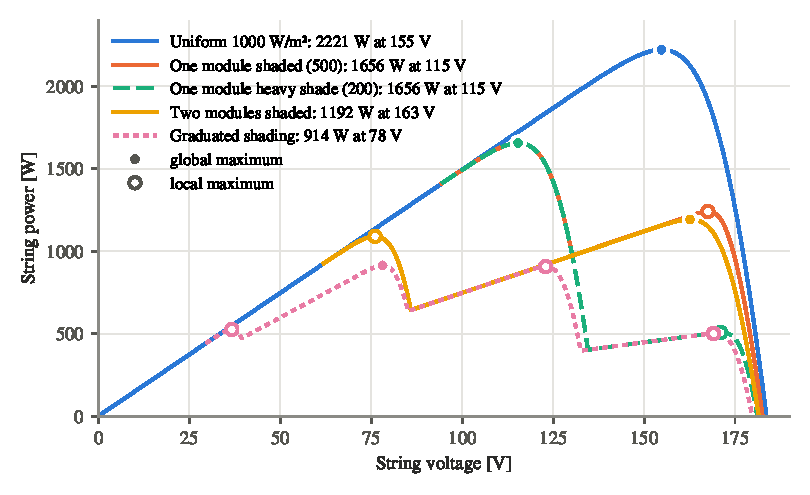
\includegraphics[width=0.85\linewidth]{misc/pv_shading}
  \caption{P--V curves of a four-module string (AIKO Neostar A555, single-diode model with bypass diodes) under five irradiance patterns.}
  \label{fig:pvmismatch}
\end{figure}

\begin{table}[htbp]
  \centering
  \small
  \caption[{Mismatch loss of the shaded strings}]{Mismatch loss of the shaded strings in \cref{fig:pvmismatch}: string global maximum against the sum of the modules' individual maxima (the power a lossless per-module tracker could extract).}
  \label{tab:pvshading}
  \begin{tabular}{l c r r r}
    \toprule
    Scenario & Irradiance [W/m$^2$] & Module MPPs [W] & String MPP [W] & Loss \\
    \midrule
    Uniform                 & 1000, 1000, 1000, 1000 & 2221 & 2221 & 0.0\,\% \\
    One module shaded       & 1000, 1000, 1000, 500  & 1944 & 1656 & 14.8\,\% \\
    One module heavy shade  & 1000, 1000, 1000, 200  & 1775 & 1656 & 6.7\,\% \\
    Two modules shaded      & 1000, 1000, 500, 500   & 1667 & 1193 & 28.5\,\% \\
    Graduated shading       & 1000, 800, 500, 200    & 1388 & 914  & 34.1\,\% \\
    \bottomrule
  \end{tabular}
\end{table}

Array reconfiguration (series-parallel, bridge-linked and total-cross-tied) reduces this mismatch loss but cannot remove it \cite{rao_maximum_2014}. Bypass diodes protect the shaded cells, but at the cost of a multi-peaked P--V curve and the energy of every bypassed module. Recovering that energy requires moving power between the modules themselves.

\subsection{Existing shuffler concepts: DPP and S-PPC}
\label{sec:lit_dpp}
The power shuffler is part of the family of differential power processors (DPP) \cite{kasper_classification_2014}, whose reason for being is to move differences in power around a system, effectively balancing out either voltage or current. The serial partial power converter (S-PPC) specialises in moving the power differentials of modules that are connected in series \cite{jeong_segmented_2020}.

The idea has a long history at QUT: Walker, Xue and Sernia first proposed per-module ``shuffling'' converters that let each module in a string operate at its own maximum power point \cite{walker_pv_2003}. Hui's later QUT work documents why this matters outside the lab \cite{hui_development_2020}. Shufflers of a very different design were fitted to ATN's solar car \emph{Priscilla} for the 2019 Bridgestone World Solar Challenge. IN a prestigious challenge such as this every watt matters. The curvature of the 1.25\,kW array and obstacles passing overhead shade it unevenly while driving. Drops in performance of these solar panels translate to reduced speed and cruise time in this endurance race. The design was rushed into the car under tight timelines with limited testing, the devices did not perform reliably and ultimately failed during the challenge, and the follow-on work was redirected to making them operate safely and reliably. It is a clear reminder that protection and safety features have to be designed into a shuffler from the start (\cref{sec:risks}). Kasper et al.\ classify panel-integrated DC--DC concepts and identify the buck-boost as the most promising \cite{kasper_classification_2014,kasper_impact_2014}. Olalla et al.\ formalise the modelling of DPP architectures and show near-ideal energy extraction with converter ratings that scale with the mismatch rather than the string power \cite{olalla_modeling_2014,olalla_performance_2014}. Jeong et al.\ review DPP architectures \cite{jeong_review_2018} and demonstrate a four-unit segmented DPP experimentally \cite{jeong_segmented_2020}; Li and Cobos give a framework for comparing the VA ratings of partial power converters \cite{li_classification_2021}; and dos Santos et al.\ present a practical two-switch S-PPC \cite{dos_santos_two-switch_2021}. A common thread runs through these works: their focus is the power stage and the architecture, and the control is either not discussed or kept simple and classical, with a PI loop on a single unit.

The S-PPC used in this project is the interleaved buck-boost converter: two half-bridge legs joined through a coupled inductor to the midpoint between two series modules (\cref{fig:shuffler}). At a duty of $D=0.5$ the midpoint sits at half the pair voltage; moving $D$ away from 0.5 moves current from one module to the other, and in steady state the current circulating between the two phases should be zero.

\subsection{Controlling the interleaved buck-boost}
\label{sec:lit_control}
A single buck-boost converter is described by one second-order ordinary differential equation (ODE), and classical frequency-domain design works well for it. Interleaving changes this the presence of a second phase and the coupled inductance couple the states (ie. PV module voltages and the currents through each inductor winding), so they cannot be controlled independently \cite{milasi_robust_2024}. Kabalci and Boyar add an extended Kalman filter to an interleaved boost converter to handle these coupled states \cite{kabalci_highly_2022}, and the behaviour of coupled inductors in interleaved converters is treated in \cite{huang_high-frequency_2015,guacci_experimental_2019}.

State-space methods handle this coupling naturally. Batzelis et al.\ give a six-state representation of irradiance-driven PV dynamics that includes the boost converter, the PI integrator and the MPPT reference \cite{batzelis_state-space_2018}; this is the modelling style adopted here, extended with the shuffler's winding dynamics. Other state-space MPPT work reports that LQR and LQR-PI controllers outperform P\&O \cite{lin_state-space_2021,khan_state-space_2024,assabaa_enhancing_2025}.

\subsection{Modelling, simulation and test methods}
\label{sec:lit_methods}
Switching converters are normally designed for control with averaged models. State-space averaging replaces the switched circuit with a continuous-time model whose inputs are the duty cycles \cite{middlebrook_general_1976}, and Kassakian et al.\ develop averaged and linearised models of the buck-boost family as the basis for its control design \cite{kassakian_principles_2024}. Averaging discards the switching ripple, so the model is valid only well below the switching frequency, and it says nothing about dead time, sampling delay or sensor noise.

The simulation tools follow from those two limits. Simulink is the standard environment for model-based design: the controller and an averaged plant run together in one model, which makes it the natural tool for model-in-the-loop (MIL) verification on the left of the V-model \cite{mathworks_simulink_2026,seal_system_2018}. QSPICE is a switching-level SPICE simulator with built-in C++ compilation, so compiled C code can run as a block inside the circuit \cite{qorvo_qspice_2023}. That allows the firmware's own control core to be tested against real switches, drivers, dead time and sensing models before it reaches hardware, closing the gap the averaged model leaves.

For experimental testing, MPPT performance is standardised: EN~50530 defines dynamic test sequences of irradiance ramps for measuring tracking efficiency, and Li et al.\ use them to compare MPPT algorithms experimentally \cite{li_comparative_2021}. Riquelme-Dom\'inguez and Mart\'inez evaluate MPPT algorithms on state-space models under several such dynamic test procedures \cite{riquelme-dominguez_systematic_2022}. These procedures need a programmable PV simulator. This project draws on the same approach, repeatable steps on the bench with programmable supplies and an electronic load followed by validation on a real string outdoors, but a full EN~50530 campaign is outside its scope.

\subsection{The gap}
\label{sec:gap}
Past controllers have been able to rely on classical methods such as PI because each controls a single converter. Multiple-input multiple-output (MIMO) control of a string of coupled shufflers has had very limited exploration, and control of the interleaved buck-boost converter is itself a niche topic. To the author's knowledge, no published work models an $N$-module string of interleaved buck-boost DPP converters as one MIMO plant, identifies its DC gain matrix and closes a decoupling integral controller on real hardware, with the module-voltage differences and circulating currents as outputs. This project does that, carrying the design through analytical, Simulink, QSPICE, firmware, bench and solar phases, and reports the same metrics for every phase on one set of test cases.

\section{Methodology}
\label{sec:method}

% ---- Talking points written up as prose (your version: 05_methodology_draft.tex).

\subsection{Controller Design Pipeline}
\label{sec:pipeline}
The methods applied to the project correspond to the stages of the V-model in \cref{fig:vmodel}. It is a way for systems engineers to map out development across a product's life cycle \cite{seal_system_2018}. The first step in the design process is to determine the target use case and application of the product through background research, refining project objectives. To determine the system requirements for a controller the plant is modelled. The controller algorithms are then adpated to Simulink where a high-level structure forms. Based on this abstract model, components are selected for the controller PCB based on the requirements of the controller architecture. Selecting marketplace controllers and sensors, opens the door for firmware development because now there is a defined interface. The firmware's control code is then combined with the plant models in software-in-the-loop and QSPICE simulations, which give a theoretical approximation of the experiments. The system is tested in the electronics lab, and finally outdoors with a string of three PV modules, which is the core objective and ultimate validation of the system. \Cref{tab:phases} (\cref{app:timeline}) links each phase to its V-model counterpart and its primary artefact.

\begin{figure}[htbp]
  \centering
  % Controller design pipeline mapped onto the systems-engineering V-model.
% Drawn at print size (text width 17 cm): include without \resizebox.
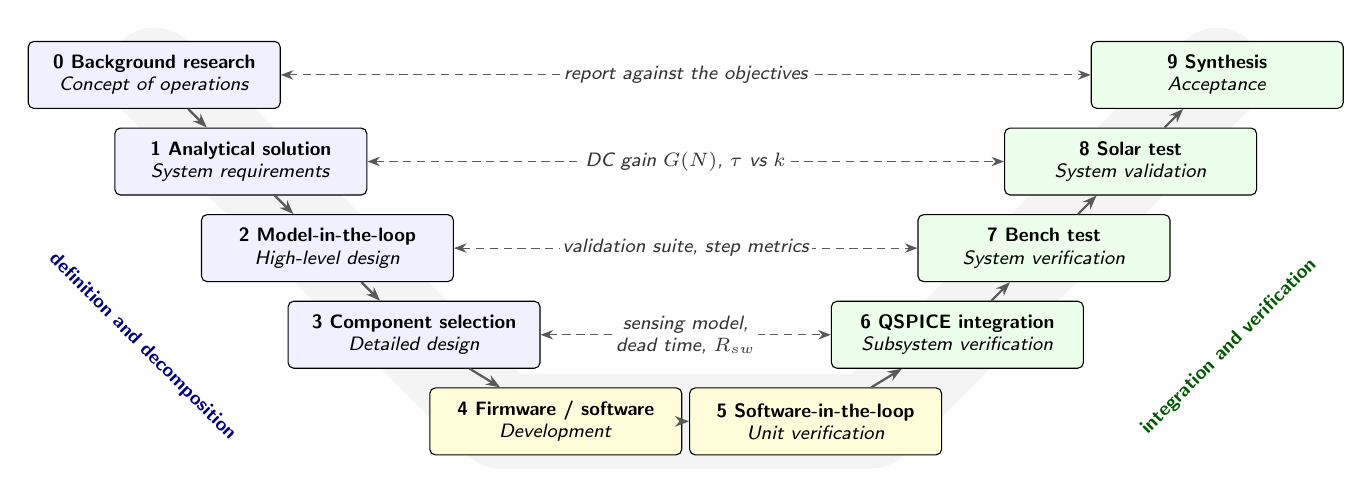
\begin{tikzpicture}[x=1cm,y=1cm,font=\sffamily\scriptsize,
    ph/.style={draw,rounded corners=2pt,minimum width=32mm,minimum height=8.5mm,align=center,inner sep=2pt},
    arm/.style={-{Stealth[length=1.8mm]},thick,gray!70!black},
    ver/.style={{Stealth[length=1.6mm]}-{Stealth[length=1.6mm]},densely dashed,gray!70!black},
    vlab/.style={fill=white,inner sep=1pt,align=center,font=\sffamily\scriptsize\itshape,text=gray!40!black}]
  % the V itself: a band through the box centres
  \begin{scope}[on background layer]
    \draw[line width=12mm,gray!9,line cap=round,line join=round] (1.75,4.4) -- (6.15,0) -- (10.85,0) -- (15.25,4.4);
  \end{scope}
  % left arm: definition and decomposition (45 degrees)
  \node[ph,fill=blue!6]   (p0) at (1.75,4.4) {\textbf{0 Background research}\\\textit{Concept of operations}};
  \node[ph,fill=blue!6]   (p1) at (2.85,3.3) {\textbf{1 Analytical solution}\\\textit{System requirements}};
  \node[ph,fill=blue!6]   (p2) at (3.95,2.2) {\textbf{2 Model-in-the-loop}\\\textit{High-level design}};
  \node[ph,fill=blue!6]   (p3) at (5.05,1.1) {\textbf{3 Component selection}\\\textit{Detailed design}};
  % base of the V
  \node[ph,fill=yellow!15] (p4) at (6.85,0)  {\textbf{4 Firmware / software}\\\textit{Development}};
  \node[ph,fill=yellow!15] (p5) at (10.15,0) {\textbf{5 Software-in-the-loop}\\\textit{Unit verification}};
  % right arm: integration and verification
  \node[ph,fill=green!8]  (p6) at (11.95,1.1) {\textbf{6 QSPICE integration}\\\textit{Subsystem verification}};
  \node[ph,fill=green!8]  (p7) at (13.05,2.2) {\textbf{7 Bench test}\\\textit{System verification}};
  \node[ph,fill=green!8]  (p8) at (14.15,3.3) {\textbf{8 Solar test}\\\textit{System validation}};
  \node[ph,fill=green!8]  (p9) at (15.25,4.4) {\textbf{9 Synthesis}\\\textit{Acceptance}};
  % flow along the arms
  \foreach \a/\b in {p0/p1,p1/p2,p2/p3,p6/p7,p7/p8,p8/p9}{\draw[arm] (\a) -- (\b);}
  \draw[arm] (p3) -- (p4);
  \draw[arm] (p4) -- (p5);
  \draw[arm] (p5) -- (p6);
  % arm labels
  \node[rotate=-45,font=\sffamily\scriptsize\bfseries,text=blue!50!black] at (1.6,0.95) {definition and decomposition};
  \node[rotate=45,font=\sffamily\scriptsize\bfseries,text=green!35!black] at (15.4,0.95) {integration and verification};
  % verification pairs across the V
  \draw[ver] (p0) -- node[vlab]{report against the objectives} (p9);
  \draw[ver] (p1) -- node[vlab]{DC gain $G(N)$, $\tau$ vs $k$} (p8);
  \draw[ver] (p2) -- node[vlab]{validation suite, step metrics} (p7);
  \draw[ver] (p3) -- node[vlab]{sensing model,\\dead time, $R_{sw}$} (p6);
\end{tikzpicture}

  \caption[{Controller design pipeline mapped onto the systems-engineering V-model}]{Controller design pipeline mapped onto the systems-engineering V-model. Dashed links are the verification pairs used in \cref{sec:synthesis}.}
  \label{fig:vmodel}
\end{figure}
This method suits the problem because every phase produces a pass/fail artefact that the next phase consumes (model, then gains, then \code{params.h}, then the bench), so a fault is isolated at the level where it was introduced. The C control core is the same source file in software-in-the-loop, in QSPICE and in the firmware, so what is simulated is what is deployed.

The work was divided between control and power electronics. The hardware teammate, Son Nguyen, owned the power stage, the QSPICE schematic and the PCB layout. This project owned the control. The hand-over interface between the two was the QSPICE schematic and the sensor set. The team was proactive with regular progress updates occurring often more than twice a week. The supervisor, Assoc.\ Prof.\ Walker was updated eveyr fortnight either via email or in-person meetings.

Every bench and solar run was logged as telemetry at about 44\,Hz into InfluxDB, alongside the electronic load's own log at 5\,Hz. Grafana screenshots defined the test windows, and the analysis pipeline re-exports those windows and computes every metric from the same CSV files (\cref{sec:synthesis}).

\subsection{Background}
\label{sec:background}
\Cref{fig:shuffler} shows one shuffler drawn in the variables of the $N$-module model. Its two half-bridge legs, phase A and phase B, switch between the top rail $\phi_j$ and the bottom rail $\phi_{j+2}$ at duties $d_A$ and $d_B$, and each switch node drives one winding of a coupled inductor whose common end is tied to the midpoint $\phi_{j+1}$ between the two modules. The capacitors $C_j$ and $C_{j+1}$ decouple the modules from the switching ripple. The sum of the winding currents, the shuffled current $\im = i_A + i_B$, moves charge between the two modules. Their difference, the circulating current $\ic = i_A - i_B$, flows only around the two legs: it moves no power between the modules and is pure loss, so it is regulated to zero. In steady state the two legs switch 180$^\circ$ apart at the same duty, and the duty sets the ratio of the two module voltages.

\begin{figure}[htbp]
  \centering
  % One interleaved buck-boost power shuffler j between modules j and j+1 (layout after the
% EGH490-1 progress report, Fig. 1), in the variables of the N-module model.  Print size.
\begin{circuitikz}[american,font=\footnotesize,x=0.96cm,y=1cm,
    pwm/.pic={\draw[thin] (0,0) -- (0,0.22) -- (0.16,0.22) -- (0.16,0) -- (0.32,0) -- (0.32,0.22) -- (0.48,0.22) -- (0.48,0);},
    phbox/.style={draw,densely dashed,rounded corners=4pt,gray!70!black,inner sep=4pt}]
  \def\yT{5}\def\yM{2.65}\def\yB{0}
  % ---------------- phase B leg (x = 2.0) and phase A leg (x = 6.0)
  \foreach \x/\p in {2.0/B,6.0/A}{
    \draw (\x,\yT) node[nmos,bodydiode,anchor=D] (QH\p) {};
    \draw (QH\p.S) -- (\x,3.15) coordinate (sw\p);
    \draw (\x,2.2) node[nmos,bodydiode,anchor=D] (QL\p) {};
    \draw (QL\p.S) -- (\x,\yB);
    \draw (QH\p.G) -- ++(-0.35,0) coordinate (gH\p);
    \draw (QL\p.G) -- ++(-0.35,0) coordinate (gL\p);
    \pic at ($(gH\p)+(-0.62,-0.11)$) {pwm};
    \pic at ($(gL\p)+(-0.62,-0.11)$) {pwm};
    \draw (sw\p) -- (\x,2.2);
  }
  \node[left,font=\scriptsize] at ($(gHB)+(-0.65,0)$) {$d_B$};
  \node[left,font=\scriptsize] at ($(gLB)+(-0.65,0)$) {$1-d_B$};
  \node[left,font=\scriptsize] at ($(gHA)+(-0.65,0)$) {$d_A$};
  \node[left,font=\scriptsize] at ($(gLA)+(-0.65,0)$) {$1-d_A$};
  \node[phbox,fit={(-0.55,4.95) (2.45,0.25)},label={[font=\footnotesize\sffamily]below:Phase B}] {};
  \node[phbox,fit={(3.45,4.95) (6.45,0.25)},label={[font=\footnotesize\sffamily]below:Phase A}] {};
  % rails
  \draw (2.0,\yT) -- (14.7,\yT);
  \draw (2.0,\yB) -- (14.7,\yB);
  \fill (6.0,\yT) circle (1.5pt) (6.0,\yB) circle (1.5pt);
  % ---------------- coupled windings: switch nodes -> midpoint phi_{j+1}
  \draw (swA) node[circ]{} -- (6.7,3.15) -- (6.7,3.6) to[short,i=$i_A$] (7.3,3.6) to[cute inductor,l=$L_A$] (8.9,3.6) -- (9.6,3.6) -- (9.6,\yM);
  \draw (2.0,2.55) node[circ]{} -- (5.8,2.55) arc[start angle=180,end angle=0,radius=0.2] -- (6.7,2.55) -- (6.7,2.1)
        to[short,i=$i_B$] (7.3,2.1) to[cute inductor,l_=$L_B$] (8.9,2.1) -- (9.6,2.1) -- (9.6,\yM);
  % dots: anti-series (1:-1) coupling as built
  \fill (7.45,3.95) circle (1.6pt);  \fill (8.75,1.75) circle (1.6pt);
  \draw[<->,thin] (8.1,3.3) -- node[right=1pt,font=\scriptsize]{$M$} (8.1,2.4);
  \node[font=\scriptsize,align=left,anchor=north west] at (6.6,0.95)
       {$i_m = i_A + i_B$ (shuffled, into $\phi_{j+1}$)\\$i_c = i_A - i_B$ (circulating)};
  % ---------------- midpoint, decoupling capacitors, modules
  \draw (9.6,\yM) node[circ]{} -- (14.7,\yM);
  \draw (10.7,\yT) to[C,l_=$C_j$,*-*] (10.7,\yM) to[C,l_=$C_{j+1}$,-*] (10.7,\yB);
  \draw (12.2,\yM) to[pvsource,l_=$I_j$,*-*] (12.2,\yT);
  \draw (12.2,\yB) to[pvsource,l_=$I_{j+1}$,*-*] (12.2,\yM);
  \draw (13.95,\yT) to[open,v^>=$v_j$] (13.95,\yM);
  \draw (13.95,\yM) to[open,v^>=$v_{j+1}$] (13.95,\yB);
  \node[ocirc] at (14.7,\yT) {}; \node[ocirc] at (14.7,\yM) {}; \node[ocirc] at (14.7,\yB) {};
  \node[right,align=left] at (14.75,\yT) {$\phi_j$\\[-1pt]{\scriptsize top rail}};
  \node[right,align=left] at (14.75,\yM) {$\phi_{j+1}$\\[-1pt]{\scriptsize midpoint}};
  \node[right,align=left] at (14.75,\yB) {$\phi_{j+2}$\\[-1pt]{\scriptsize bottom rail}};
  \node[font=\scriptsize\sffamily] at (12.2,5.45) {modules $j$, $j+1$};
\end{circuitikz}

  \caption[{One interleaved buck-boost power shuffler between modules $j$ and $j+1$}]{One interleaved buck-boost power shuffler $j$ between modules $j$ and $j+1$ (layout after the progress report). The two legs drive anti-series coupled windings $L_A$, $L_B$ into the midpoint $\phi_{j+1}$; $C_j$, $C_{j+1}$ decouple the modules from the switching ripple.}
  \label{fig:shuffler}
\end{figure}

The target system is two shufflers, one controller, a telemetry system and a user interface on a string of three PV modules. Three is the minimum needed to show shufflers interacting in a string, and the foundation for scaling. The early designs were rated to the highest-rated commercial panel available, the AIKO Neostar 555\,W ($V_{mp}$ 38.7\,V, $I_{mp}$ 14.35\,A), so that the controller would never be the limiting element. The outdoor experiment used 80\,W KickAss KAUSSP80 panels \cite{kaussp80_ds} for safety and availability, and the models carry both parameter sets.

Each shuffler has two control inputs, the common-mode duty $\uc = d_A + d_B - 1$ and the differential-mode duty $\ud = d_A - d_B$, and two controlled outputs, the voltage difference $\vd{}_{,j} = v_j - v_{j+1}$ and the circulating current $\ic{}_{,j}$. With $N-1$ shufflers on $N$ modules, every module except the two at the ends is shared by two shufflers, so each $\uc$ moves two module voltages and the plant is a coupled ladder and thus the control problem is multiple-input multiple-output.

\subsection{Analytical Solution}
\label{sec:analytical}

\subsubsection*{Single shuffler (Semester 1 model, \cref{app:single})}
The Semester 1 model describes one shuffler with the state $x = [I_{L1}, I_{L2}, V_{C1}, V_{C2}]^T$, the duties $[d_A, d_B]^T$ as inputs and the module and load currents as disturbances, averaging the four dual-switch states. Three insights of that analysis were preserved. The equilibrium requires $D_A = D_B = D$ with $\bar V_{C2}/\bar V_{C1} = D/(1-D)$. Without parasitics the plant is marginally stable, with an undamped resonance at 5.56\kHz, and even with the winding resistance the damping ratio is only about 0.0025, which is why the early classical designs did not work. Finally, the module voltages alone make only three of the four states observable (the difference current is hidden), so per-phase current sensing is mandatory, which fixed the sensor set (\cref{sec:components}). The coupling between the states also ruled out three cascaded single-loop controllers. The problem is multiple-input multiple-output. It was first approached with an LQR and integral regulator and then with the decoupling PI controller that was deployed.

\subsubsection*{Where the winding equations come from}
\Cref{fig:coupled}(a) replaces each leg with its averaged switch-node voltage $\phi_{j+2} + d\,\Vbar_j$, where $\Vbar_j = v_j + v_{j+1}$ is the voltage across the pair, so each winding sees $d\,\Vbar_j - v_{j+1}$ less its resistive drop. The windings are anti-series as built (turns 1:$-1$), so $v_A = L\,\dot i_A - M\,\dot i_B$ and $v_B = L\,\dot i_B - M\,\dot i_A$. Adding and subtracting the two winding equations, and using $\Vbar_j - 2v_{j+1} = v_j - v_{j+1} = \vd{}_{,j}$, gives the two mode equations of the deployed model:
\begin{align}
  (L-M)\,\dot\im{}_{,j} &= \Vbar_j\,\uc{}_{,j} + \vd{}_{,j} - R_m\,\im{}_{,j} \label{eq:wind1}\\
  (L+M)\,\dot\ic{}_{,j} &= \Vbar_j\,\ud{}_{,j} - R_c\,\ic{}_{,j} \label{eq:wind2}
\end{align}
The coupled inductor therefore splits into two independent modes (\cref{fig:coupled}(b, c)). The shuffled current sees only the leakage inductance $L - M = 2.05\uH$ and the circulating current the full $L + M = 13.75\uH$ ($L = 7.9\uH$ and $M = 5.85\uH$ per winding as built, from the ERUC23's 2.05\,$\mu$H leakage and 5.85\,$\mu$H magnetising inductance \cite{tdk_eruc23_ds}). The common-mode duty drives the voltage mode, the differential-mode duty drives the current mode, and to first order the two do not interact, which is the structure the decoupling controller exploits. In the averaged model $R_m = R_c = R_w$; on the switching hardware $R_c$ also contains the switching resistance $R_{sw}$ (\cref{sec:gainpipe}).

\begin{figure}[htbp]
  \centering
  % Where the winding equations come from: averaged half-bridges driving the anti-series coupled
% windings into the midpoint (left) and the two decoupled modes (right).  Print size.
\begin{circuitikz}[american,font=\footnotesize,x=1cm,y=1cm]
  % ------------------------------------------------ (a) averaged shuffler around the midpoint
  \draw (0,0) to[V,l=$d_A\bar V_j$,invert] (0,2.6)
        to[short,i=$i_A$] (0.6,2.6) to[R,l=$R_w$] (2.0,2.6) to[cute inductor,l=$L$] (3.4,2.6) -- (4.2,2.6) coordinate (M);
  \draw (8.4,0) to[V,l_=$d_B\bar V_j$,invert] (8.4,2.6)
        to[short,i_=$i_B$] (7.8,2.6) to[R,l_=$R_w$] (6.4,2.6) to[cute inductor,l_=$L$] (5.0,2.6) -- (M);
  \draw (M) node[circ]{} node[above=2pt]{$\phi_{j+1}$} to[V,l=$v_{j+1}$] (4.2,0);
  \draw (0,0) -- (8.4,0);
  \node[below] at (4.2,0) {$\phi_{j+2}$ (bottom rail)};
  \fill (2.15,2.95) circle (1.6pt);  \fill (5.15,2.95) circle (1.6pt);
  \draw[<->,thin] (2.9,3.15) to[bend left=25] node[above,font=\scriptsize]{$M$, anti-series} (5.5,3.15);
  \node[font=\sffamily\footnotesize] at (4.2,4.2) {(a) averaged legs and coupled windings};
  \node[font=\scriptsize,align=center,text=gray!30!black] at (4.2,-1.15)
       {each leg's switch node averages to $\phi_{j+2} + d\,\bar V_j$;\\$v_{A} = L\,\dot i_A - M\,\dot i_B$, \ $v_{B} = L\,\dot i_B - M\,\dot i_A$};
  % ------------------------------------------------ (b) the two modes
  \begin{scope}[shift={(10.6,2.0)}]
    \draw (0,0) to[V,l_=$\bar V_j u_c + v_{d,j}$,invert] (0,1.8) to[short,i=$i_m$] (0.7,1.8)
          to[R,l=$R_m$] (2.3,1.8) to[cute inductor,l=$L-M$] (4.0,1.8) -- (4.0,0) -- (0,0);
    \node[font=\sffamily\footnotesize,anchor=west] at (-0.6,2.85) {(b) shuffled mode $i_m = i_A + i_B$};
  \end{scope}
  \begin{scope}[shift={(10.6,-1.45)}]
    \draw (0,0) to[V,l_=$\bar V_j u_d$,invert] (0,1.8) to[short,i=$i_c$] (0.7,1.8)
          to[R,l=$R_c$] (2.3,1.8) to[cute inductor,l=$L+M$] (4.0,1.8) -- (4.0,0) -- (0,0);
    \node[font=\sffamily\footnotesize,anchor=west] at (-0.6,2.85) {(c) circulating mode $i_c = i_A - i_B$};
  \end{scope}
\end{circuitikz}

  \caption[{Origin of the winding equations}]{Where the winding equations come from. (a) Each leg averaged to $d\,\Vbar_j$ above the bottom rail, driving one of the anti-series coupled windings into the midpoint. (b, c) Adding and subtracting the two winding equations splits them into the shuffled mode, which sees $L-M$, and the circulating mode, which sees $L+M$ (\cref{eq:wind1,eq:wind2}).}
  \label{fig:coupled}
\end{figure}

\subsubsection*{The string as a nodal network}
\Cref{fig:nodal} draws the small-signal network of a three-module string. Each module $k$ is linearised about its operating point into a current source $I_k$ in parallel with its slope conductance $g_k = -\mathrm{d}I/\mathrm{d}V$ and the capacitance $C_k$ across it. Node 4 is ground, and the DL3021 in constant-voltage mode appears as a large conductance $G_{load}$ across the string. Each shuffler enters only through its injections: averaged over a period, it pushes $\im{}_{,j}$ into its midpoint and draws $\tfrac12\im{}_{,j}$ from each rail. Kirchhoff's current law at the nodes gives
\begin{equation}
  C_n\,\dot\phi = -G_n\,\phi + S\,\im + w, \qquad \vd = D_v\,\phi, \label{eq:nodal}
\end{equation}
which for $N = 3$, with $w = [I_1,\; I_2 - I_1,\; I_3 - I_2]^T$ the module current injections, reads
\begin{gather*}
  C_n = \begin{bmatrix} C_1 & -C_1 & 0\\ -C_1 & C_1{+}C_2 & -C_2\\ 0 & -C_2 & C_2{+}C_3\end{bmatrix},\qquad
  G_n = \begin{bmatrix} g_1{+}G_{load} & -g_1 & 0\\ -g_1 & g_1{+}g_2 & -g_2\\ 0 & -g_2 & g_2{+}g_3\end{bmatrix},\\[4pt]
  S = \begin{bmatrix} -\tfrac12 & 0\\ 1 & -\tfrac12\\ -\tfrac12 & 1\end{bmatrix},\qquad
  D_v = \begin{bmatrix} 1 & -2 & 1\\ 0 & 1 & -2\end{bmatrix}.
\end{gather*}
The same pattern holds for any $N$: $C_n$ and $G_n$ are tridiagonal Laplacians of the module capacitances and conductances, each shuffler adds one column $[-\tfrac12, 1, -\tfrac12]$ to $S$, and each row of $D_v$ forms $\vd{}_{,j} = \phi_j - 2\phi_{j+1} + \phi_{j+2}$. For the solar string, $C = [130, 260, 130]\uF$ (the middle module carries the decoupling capacitors of both shufflers), $g = 0.19$\,S per module and $G_{load} = 20$\,S.

\begin{figure}[htbp]
  \centering
  % Small-signal nodal model of a 3-module string with two shufflers (the matrices of eq. nodal).
% Print size.
\begin{circuitikz}[american,font=\footnotesize,x=1cm,y=1cm,
    shb/.style={draw,rounded corners=3pt,fill=orange!8,minimum width=12mm,align=center,font=\scriptsize\sffamily}]
  \def\xa{0.6}\def\xb{1.9}\def\xc{3.2}
  % node rails
  \foreach \k/\y/\xs/\xe in {1/6/-1.6/5.65,2/4/-0.3/8.45,3/2/-0.3/8.45,4/0/-1.6/8.45}{
    \draw (\xs,\y) -- (\xe,\y);
    \node[left] at (\xs-0.1,\y) {$\phi_{\k}$};
  }
  \node[left,font=\scriptsize,text=gray!30!black] at (-1.7,-0.4) {(ground)};
  % modules k between phi_k and phi_{k+1}: I_k || g_k || C_k
  \foreach \k/\yt/\yb in {1/6/4,2/4/2,3/2/0}{
    \draw (\xa,\yb) to[I,l=$I_{\k}$,*-*] (\xa,\yt);
    \draw (\xb,\yt) to[R,l=$g_{\k}$,*-*] (\xb,\yb);
    \draw (\xc,\yt) to[C,l=$C_{\k}$,*-*] (\xc,\yb);
    \draw[decorate,decoration={brace,amplitude=4pt,mirror},thin] (4.25,\yb+0.1) -- node[right=4pt]{$v_{\k}$} (4.25,\yt-0.1);
  }
  % CV load across the string
  \draw (-1.0,6) to[R,l_=$G_{load}$,*-*] (-1.0,0);
  % shuffler 1: rails phi_1, phi_3, midpoint phi_2
  \node[shb,minimum height=44mm] (S1) at (6.3,4) {shuffler\\1\\[2pt]$u_{c,1}$\\$u_{d,1}$};
  \draw (S1.west |- 0,6) to[short,i<_=$\tfrac12 i_{m,1}$,-*] (5.0,6);
  \draw (S1.west |- 0,4) to[short,i=$i_{m,1}$,-*] (5.0,4);
  \draw (S1.west |- 0,2) to[short,i<=$\tfrac12 i_{m,1}$,-*] (5.0,2);
  % shuffler 2: rails phi_2, phi_4, midpoint phi_3
  \node[shb,minimum height=44mm] (S2) at (9.1,2) {shuffler\\2\\[2pt]$u_{c,2}$\\$u_{d,2}$};
  \draw (S2.west |- 0,4) to[short,i<_=$\tfrac12 i_{m,2}$,-*] (7.8,4);
  \draw (S2.west |- 0,2) to[short,i=$i_{m,2}$,-*] (7.8,2);
  \draw (S2.west |- 0,0) to[short,i<=$\tfrac12 i_{m,2}$,-*] (7.8,0);
  \node[font=\scriptsize,align=left,anchor=north west,text=gray!30!black] at (5.6,-0.45)
       {rail currents $\tfrac12 i_m(1\pm u_c)\pm\tfrac12 i_c u_d$,\\linearised about $u_c = 0$: $-\tfrac12 i_m$ at each rail};
\end{circuitikz}

  \caption[{Small-signal nodal model of a three-module string with two shufflers}]{Small-signal nodal model of a three-module string with two shufflers: each module is $I_k \parallel g_k \parallel C_k$ between node potentials, the CV load is $G_{load}$ across the string, and each shuffler injects $\im$ at its midpoint and draws $\tfrac12\im$ from each rail (the columns of $S$ in \cref{eq:nodal}).}
  \label{fig:nodal}
\end{figure}

\subsubsection*{Equilibrium}
At $D = \tfrac12$, charge balance on the ladder gives $T(N)\,I_m = \delta I$ with $T = \mathrm{tridiag}(-\tfrac12, 1, -\tfrac12)$ and $(\delta I)_j = I_j - I_{j+1}$, whose inverse has the closed form $T^{-1}_{jk} = \tfrac{2}{N}\min(j,k)\,(N - \max(j,k))$. Each shuffler therefore carries a weighted sum of all the mismatches, and the string current settles at the mean module current, $I_{str} = \tfrac1N\sum_k I_k$. For $N = 3$, $T^{-1} = \tfrac13\left[\begin{smallmatrix}4&2\\2&4\end{smallmatrix}\right]$. At the QSPICE bench point, where the three supply channels limit at 0.8, 1.0 and 1.3\,A, $\delta I = [-0.2, -0.3]$\,A gives $I_m = [-0.467, -0.533]$\,A against $-0.464$ and $-0.539$\,A in QSPICE, and $I_{str} = 1.033$\,A against 1.024\,A. In open loop at $D = 0.5$ the only voltage difference left is the winding drop, $\vd{}_{,j} = -R_m\im{}_{,j}$.

\subsubsection*{DC gain, and what $Z_e$ means}
At DC the capacitors carry no current, so \cref{eq:nodal} gives $\phi = G_n^{-1}(S\,\im + w)$, and the voltage differences respond to the shuffled currents through
\begin{equation}
  \vd = -Z_e\,\im + \text{const}, \qquad Z_e = -D_v\,G_n^{-1}S. \label{eq:Ze}
\end{equation}
$Z_e$ is the string's DC transfer impedance: the drop in $\vd{}_{,j}$ per ampere of shuffled current in shuffler $k$. Pushing current into a midpoint lifts it, which lowers that pair's voltage difference by an amount set by how stiff the modules are. For the three-module solar string with a stiff CV load,
\begin{equation*}
  Z_e = \frac{1}{g}\,T(3) = \begin{bmatrix} 5.26 & -2.63\\ -2.63 & 5.26\end{bmatrix}\ohm.
\end{equation*}
The diagonal is just the module's own I--V slope resistance $1/g$, and the off-diagonal term is the coupling to the neighbouring shuffler through the $\tfrac12\im$ rail currents. Setting the derivative in \cref{eq:wind1} to zero, $\Vbar\uc + \vd = R_m\im$, and eliminating $\im$ with \cref{eq:Ze} gives the voltage block of the DC gain; \cref{eq:wind2} gives the current block directly:
\begin{equation}
  G(N) = \begin{bmatrix} G_v & 0\\ 0 & \mathrm{diag}(\Vbar_j/R_c)\end{bmatrix},\qquad G_v = -(R_m I + Z_e)^{-1} Z_e\,\mathrm{diag}(\Vbar_j). \label{eq:G}
\end{equation}
Because $Z_e$ is almost two orders of magnitude larger than $R_m$ (61\,m$\Omega$), $G_v \approx -\mathrm{diag}(\Vbar_j)$. For $N = 3$ the diagonal is $-40.4\V$ per unit duty and the neighbour terms only $0.31\V$ per unit, so the string barely couples the voltage loops. On the bench, where the supplies sit in current limit ($g = 0$), $Z_e$ is unbounded and $G_v = -\mathrm{diag}(\Vbar_j)$ exactly: $-46.5\V$ per unit at 23.3\,V modules. The current block is $\Vbar/R_c = 41\V / 0.061\ohm = 672$\,A per unit in the averaged model; \cref{sec:gainpipe} explains why the hardware value is five times smaller.

\subsubsection*{Controller}
The deployed controller inverts the DC gain, $M = G^{-1}\mathrm{diag}(k_I)$, with $k_{I,v} = 2\pi\cdot150$\,s$^{-1}$ for the voltage loops and $k_{I,i} = 2\pi\cdot400$\,s$^{-1}$ for the current loops. The control law is $u = k\,(M_p e + M\xi)$ with $\xi \mathrel{+}= T_s e$, $M_p = M\,\mathrm{diag}(k_{p,v}, k_{p,i})$, $T_s = 100\us$ and a 2\,kHz first-order filter on the measurements (\cref{app:nstring}). Because $MG$ is diagonal, every loop behaves as a first-order lag with time constant $\tau = 1/(k\,k_I)$: at $k = 1$, $\tau_v = 1.06\ms$ and $\tau_i = 0.40\ms$; at the boot value $k = 0.3$, 3.5 and 1.3\ms; at $k = 0.1$, 10.6 and 4.0\ms. The gain scale $k$ (\code{kscale}) is the single run-time knob: it scales the bandwidth without changing the decoupling. The open-loop phase portraits in \cref{fig:ana_portraits} (\cref{app:analytical}) show why the real plant turned out easier to control than the Semester 1 model suggested: once the switching resistance is included, the voltage mode damps itself.

\subsection{Model-in-the-Loop (MIL)}
\label{sec:mil}
The MIL model (\cref{fig:mil}) is the controller architecture in Simulink. The power circuit is idealised with an averaged plant of four AIKO-class modules (single-diode Simscape solar cells) and three shufflers with averaged switches. For the average switches, each leg is a controlled voltage source $d\,V_{bus}$ and a controlled current source $d\,i_L$. It uses $L_{self} = 7.9\uH$, $M = 5.85\uH$, a 1.85\,m$\Omega$ winding resistance, a 61\,m$\Omega$ per-phase damping resistor and 100\,$\mu$F capacitors, with a controlled current sink driven by the MPPT reference as the load. The controller runs every 50\,$\mu$s and the supervisor and MPPT every 1\,ms, on a variable-step solver with a 100\,$\mu$s maximum step. The controller, supervisor and MPPT blocks are reproduced in \cref{fig:mil_blocks} and their pseudocode in \cref{app:pseudo}.

\begin{figure}[htbp]
  \centering
  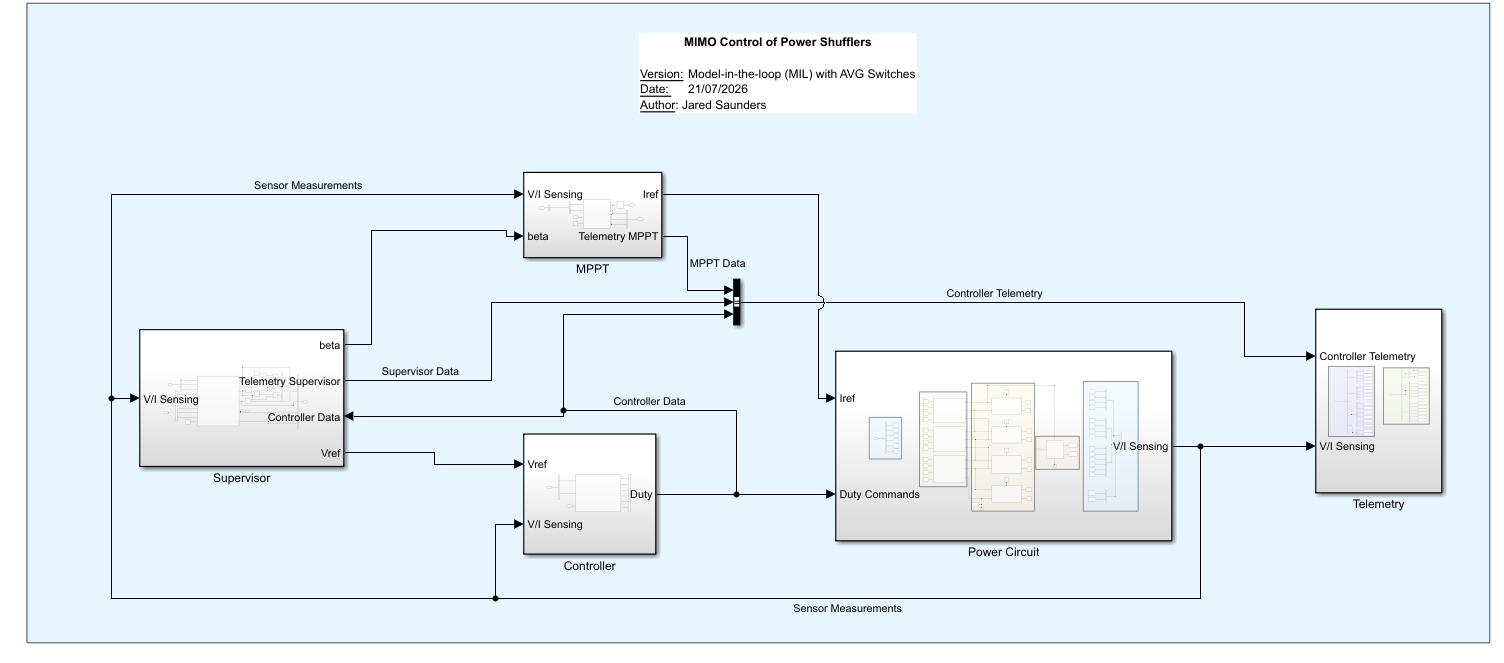
\includegraphics[width=0.92\linewidth]{img-013-015}
  \caption[{Simulink MIL model, top level}]{Simulink MIL model (\code{4\_Simulink/1\_MIL\_Model\_In\_The\_Loop}), top level: controller, supervisor, MPPT, power circuit and telemetry. The plant and the controller, supervisor and MPPT blocks are in \cref{fig:mil_plant,fig:mil_blocks}.}
  \label{fig:mil}
\end{figure}

Validation used a seven-test suite (\cref{tab:validate}): uniform irradiance, decoupling, half shade, shade with references, deep shade, MPPT under uniform irradiance and MPPT under shade. The pass criteria were $|\vd - r_v| < 0.25\V$ and $|\ic| < 1\A$ when tracking, an MPPT power of at least 98.5\,\% of the ceiling, and $|i_{diff}| \le 10\A$ in protection. All seven tests passed (\cref{tab:validate}; two are shown in \cref{fig:mil_validate}).

Software-in-the-loop (SIL) is an extension of MIL: the MATLAB Function blocks are replaced by C Caller blocks running the firmware's control core (\code{6\_RTOS/ctrl\_core}), and a bit-identical run against the MATLAB version, the golden replay, is the acceptance test. SIL is the cornerstone of the gain refinement pipeline, because the C that passes here is the C that the QSPICE DLL and the firmware compile.

\subsection{Component Selection}
\label{sec:components}
\Cref{fig:sysarch} shows the controller's data flow. The user reaches the system through the Raspberry Pi: over SSH and a parameter web page, with an IR remote, and through Grafana dashboards backed by InfluxDB, while an RGB LED and an LCD screen show the system state. The Pi flashes the Nucleo, exchanges commands and telemetry with it over UART, and reads the electronic load over USB. The Nucleo closes the loop on its own: it drives the eight PWM outputs, reads the current sensors on its ADCs and the voltage sensors over SPI, and the Pi never sits inside the control loop.

\begin{figure}[htbp]
  \centering
  % System architecture and data flow (after the presentation's controller data-flow diagram).
% Print size.
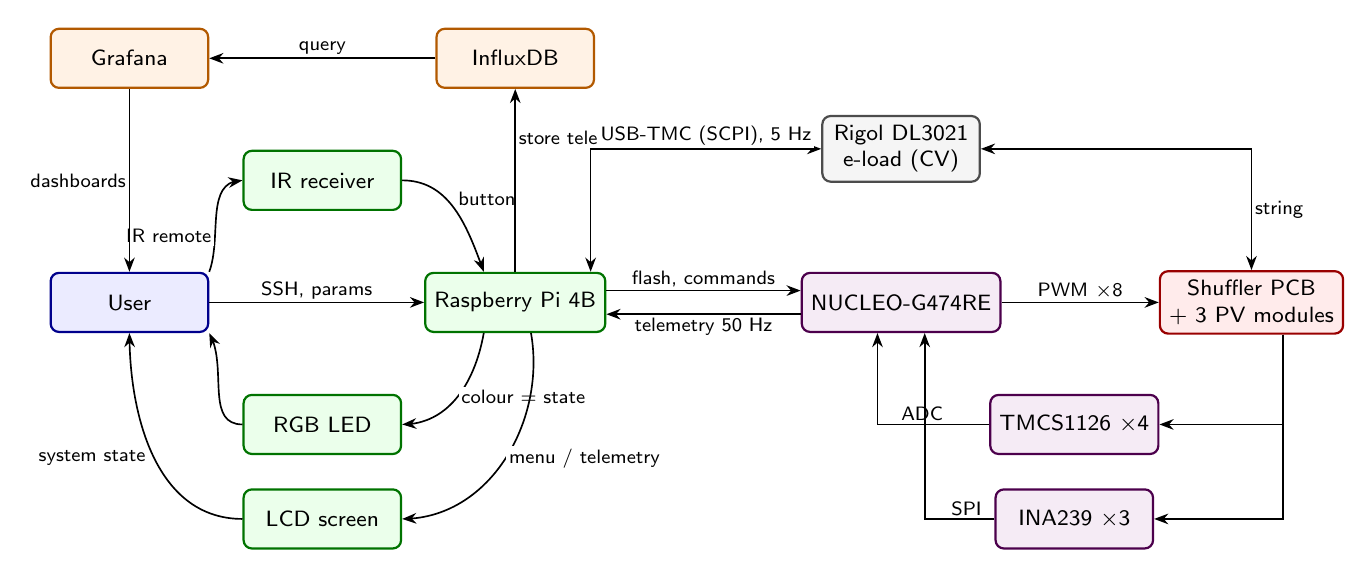
\begin{tikzpicture}[x=1cm,y=1cm,font=\sffamily\footnotesize,
    bx/.style={draw,rounded corners=3pt,minimum width=20mm,minimum height=7.5mm,align=center,thick},
    usr/.style={bx,draw=blue!55!black,fill=blue!8},
    pi/.style={bx,draw=green!45!black,fill=green!8},
    db/.style={bx,draw=orange!70!black,fill=orange!10},
    mcu/.style={bx,draw=violet!60!black,fill=violet!8},
    pl/.style={bx,draw=red!60!black,fill=red!8},
    ld/.style={bx,draw=gray!60!black,fill=gray!8},
    fl/.style={-{Stealth[length=1.8mm]},semithick},
    bl/.style={{Stealth[length=1.8mm]}-{Stealth[length=1.8mm]},semithick},
    l/.style={font=\sffamily\scriptsize,fill=white,inner sep=1pt}]
  % main row
  \node[usr] (user)  at (0,1.2)    {User};
  \node[pi]  (pi)    at (4.9,1.2)  {Raspberry Pi 4B};
  \node[mcu] (mcu)   at (9.8,1.2) {NUCLEO-G474RE};
  \node[pl]  (plant) at (14.25,1.2) {Shuffler PCB\\+ 3 PV modules};
  % Pi peripherals
  \node[pi]  (ir)    at (2.45,2.75) {IR receiver};
  \node[pi]  (led)   at (2.45,-0.35) {RGB LED};
  \node[pi]  (lcd)   at (2.45,-1.55) {LCD screen};
  % data services (Docker on the Pi)
  \node[db]  (graf)  at (0,4.3)   {Grafana};
  \node[db]  (infl)  at (4.9,4.3) {InfluxDB};
  % sensing
  \node[mcu] (cs)    at (12.0,-0.35) {TMCS1126 $\times$4};
  \node[mcu] (vs)    at (12.0,-1.55) {INA239 $\times$3};
  % electronic load
  \node[ld]  (el)    at (9.8,3.15) {Rigol DL3021\\e-load (CV)};
  % user interaction
  \draw[fl] (user) -- node[l,above]{SSH, params} (pi);
  \draw[fl] (user.north east) to[out=70,in=180] node[l,pos=0.3,left]{IR remote} (ir.west);
  \draw[fl] (ir.east) to[out=0,in=110] node[l,pos=0.5,above right]{button} ([xshift=-4mm]pi.north);
  \draw[fl] ([xshift=-4mm]pi.south) to[out=-100,in=0] node[l,pos=0.5,right]{colour = state} (led.east);
  \draw[fl] ([xshift=2mm]pi.south) to[out=-80,in=0] node[l,pos=0.5,right]{menu / telemetry} (lcd.east);
  \draw[fl] (led.west) to[out=180,in=-60] (user.south east);
  \draw[fl] (lcd.west) to[out=180,in=-90] node[l,pos=0.55,below left]{system state} (user.south);
  % logging
  \draw[fl] (pi) -- node[l,right,pos=0.72]{store telemetry} (infl);
  \draw[fl] (infl) -- node[l,above]{query} (graf);
  \draw[fl] (graf) -- node[l,left]{dashboards} (user);
  % control path
  \draw[fl] ([yshift=1.5mm]pi.east) -- node[l,above]{flash, commands} ([yshift=1.5mm]mcu.west);
  \draw[fl] ([yshift=-1.5mm]mcu.west) -- node[l,below]{telemetry 50 Hz} ([yshift=-1.5mm]pi.east);
  \draw[fl] (mcu) -- node[l,above]{PWM $\times$8} (plant);
  \draw[fl] ([xshift=4mm]plant.south) |- (cs.east);
  \draw[fl] ([xshift=4mm]plant.south) |- (vs.east);
  \draw[fl] (cs.west) -| node[l,pos=0.3,above]{ADC} ([xshift=-3mm]mcu.south);
  \draw[fl] (vs.west) -| node[l,pos=0.2,above]{SPI} ([xshift=3mm]mcu.south);
  % e-load
  \draw[bl] (el.east) -| node[l,pos=0.75,right]{string} (plant.north);
  \draw[bl] ([xshift=-2mm]pi.north east) |- node[l,pos=0.75,above]{USB-TMC (SCPI), 5 Hz} (el.west);
\end{tikzpicture}

  \caption[{Controller data flow}]{Controller data flow (after the presentation's data-flow diagram): the Raspberry Pi is the user interface, logger and flasher; the Nucleo closes the loop on its own.}
  \label{fig:sysarch}
\end{figure}

\Cref{fig:components} and \cref{tab:components} summarise the four controller components, with every figure taken from the manufacturers' datasheets. The STM32G474RE on the NUCLEO-G474RE board was chosen for its 170\,MHz clock, its five 12-bit ADCs and its high-resolution timer (HRTIM, 184\,ps resolution, with hardware dead time and complementary outputs) \cite{stm32g474_rm,mb1367_schematic}, together with its many general timers and its price; the ADC and PWM capability were the driving factors, and STM32CubeMX was used to allocate the peripherals (\cref{tab:periph_full}). The TMCS1126 Hall-effect sensor is galvanically isolated, so it can safely sit in series with the windings; the B4 variant gives 100\,mV/A about a 1.65\,V reference, a $\pm15.5$\,A linear range on a 3.3\,V supply and a 500\,kHz signal bandwidth \cite{tmcs1126_ds}. The INA239 was chosen because the higher-resolution INA229 was out of stock; it measures bus voltages up to 85\,V with a 16-bit ADC and 3.125\,mV resolution over SPI \cite{ina239_ds}. The three devices share SPI3 with separate chip selects, and their shunt inputs are tied off, so only the bus voltage and die temperature are used. The Raspberry Pi 4B \cite{rpi4_datasheet} was the safest way to add telemetry, remote control, a state display, connectivity and 5\,V / 3.3\,V distribution without adding complexity to the PCB; it hosts the web services and flashes the Nucleo, so the laptop never plugs into the system.

\begin{figure}[htbp]
  \centering
  \begin{subfigure}[b]{0.27\linewidth}\centering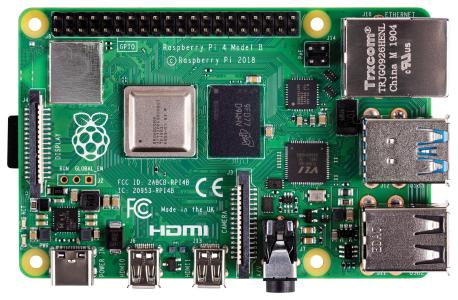
\includegraphics[height=3.0cm,keepaspectratio]{img-018-029}\caption{Raspberry Pi 4B \cite{rpi4_datasheet}}\end{subfigure}\hfill
  \begin{subfigure}[b]{0.20\linewidth}\centering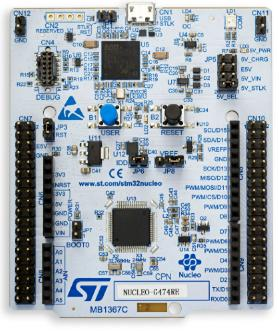
\includegraphics[height=3.0cm,keepaspectratio]{img-006-009}\caption{NUCLEO-G474RE \cite{mb1367_schematic}}\end{subfigure}\hfill
  \begin{subfigure}[b]{0.24\linewidth}\centering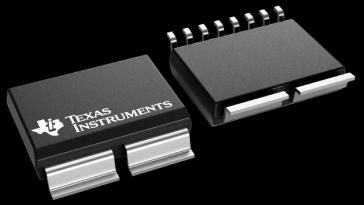
\includegraphics[width=\linewidth]{img-018-030}\caption{TMCS1126 \cite{tmcs1126_ds}}\end{subfigure}\hfill
  \begin{subfigure}[b]{0.24\linewidth}\centering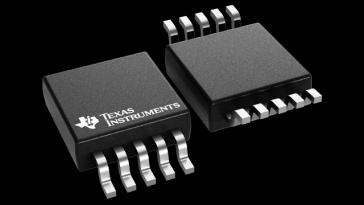
\includegraphics[width=\linewidth]{img-018-032}\caption{INA239 \cite{ina239_ds}}\end{subfigure}
  \caption[{Controller components}]{The controller components: microcomputer, microcontroller, Hall-effect current sensor and power monitor.}
  \label{fig:components}
\end{figure}

\begin{table}[htbp]\centering\small
\caption{Controller components and the datasheet figures behind their selection.}
\label{tab:components}
\begin{tabularx}{\linewidth}{l l X l}
\toprule
Role & Part & Key datasheet figures & Source\\
\midrule
Microcontroller & STM32G474RE (NUCLEO-G474RE) & Cortex-M4 at 170\,MHz; HRTIM with 184\,ps resolution, hardware dead time; five 12-bit ADCs & \cite{stm32g474_rm,mb1367_schematic}\\
Current sensor $\times$4 & TMCS1126B4AQDVGRQ1 & 100\,mV/A; $\pm15.5$\,A linear at 3.3\,V; 500\,kHz bandwidth; reinforced isolation, 5\,kV$_{\mathrm{RMS}}$ & \cite{tmcs1126_ds}\\
Voltage sensor $\times$3 & INA239AQDGSRQ1 & 0--85\,V bus input; 16-bit $\Delta\Sigma$ ADC, 3.125\,mV LSB; 10\,MHz SPI & \cite{ina239_ds}\\
Microcomputer & Raspberry Pi 4B & quad-core Cortex-A72 at 1.5\,GHz; Gigabit Ethernet, 802.11ac; 5\,V, 3\,A USB-C supply & \cite{rpi4_datasheet}\\
\bottomrule
\end{tabularx}
\end{table}

On the board (\cref{fig:routing}, \cref{app:firmware}) the ADC traces take the most direct path and are routed on the bottom layer to stay away from the switching nodes, the SPI forms a bus up and down the board, and the PWM and chip-select traces went wherever was convenient. One limitation of the Version 0 board was known before testing: the top INA239 (U10, chip select 3) sits behind an ISO7762 digital isolator that was wired backwards, so it cannot be read. The top module voltage is therefore reconstructed from the electronic load's readback, $V_{M1} = V_{str} - V_{M2} - V_{M3}$, which the Pi forwards to the Nucleo at 2\,Hz.

\subsection{Gain Refinement Pipeline}
\label{sec:gainpipe}
The gains are not tuned by hand. Each gain set starts with an identification, in which every input is stepped on a plant and the $4\times4$ DC gain matrix $G$ is measured (\cref{fig:gainpipe}). The design step turns $G$ into $M = G^{-1}\mathrm{diag}(k_I)$ and stores it, with the proportional ratios, the filter cut-off, the duty limits and a version string, in \code{shuffler\_params.json}. The generator \code{gen\_params.py} then writes \code{params.h}, which is compiled together with the same control core into all three harnesses. The version string travels in the telemetry, so every logged sample records which gain set produced it.

\begin{figure}[htbp]
  \centering
  % Gain refinement pipeline: identify G -> JSON gain set -> params.h + the one C core -> three harnesses.
% Print size.
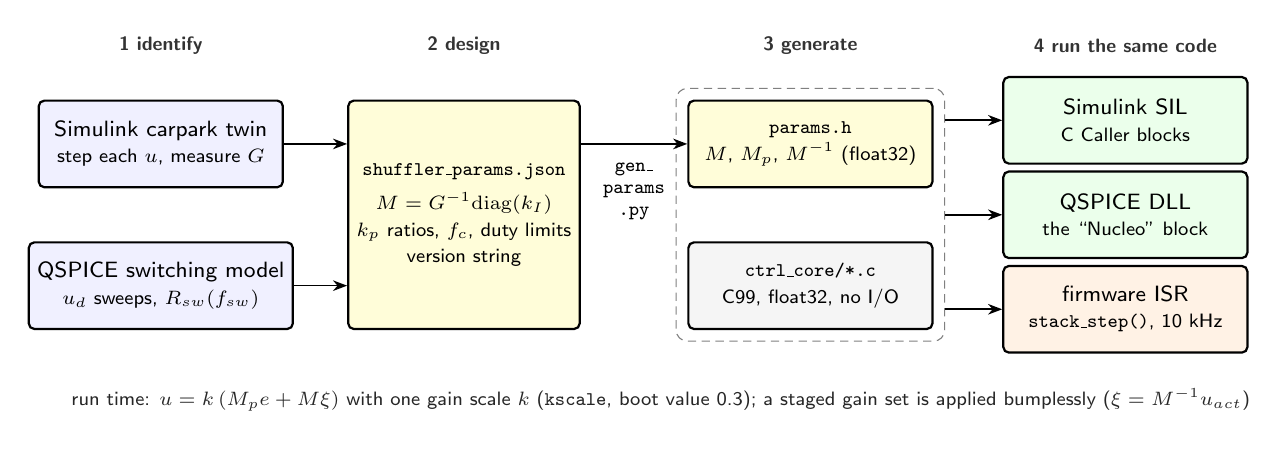
\begin{tikzpicture}[x=1cm,y=1cm,font=\sffamily\footnotesize,
    b/.style={draw,rounded corners=2pt,thick,minimum width=31mm,minimum height=11mm,align=center,inner sep=3pt},
    f/.style={-{Stealth[length=1.8mm]},semithick},
    l/.style={font=\sffamily\scriptsize,fill=white,inner sep=1pt,align=center},
    hd/.style={font=\sffamily\scriptsize\bfseries,text=gray!40!black}]
  % column headings
  \node[hd] at (1.75,2.55) {1 identify};
  \node[hd] at (5.6,2.55) {2 design};
  \node[hd] at (10.0,2.55) {3 generate};
  \node[hd] at (14.0,2.55) {4 run the same code};
  % 1 identification plants
  \node[b,fill=blue!6]   (sim) at (1.75,1.3)  {Simulink carpark twin\\{\scriptsize step each $u$, measure $G$}};
  \node[b,fill=blue!6]   (qsp) at (1.75,-0.5) {QSPICE switching model\\{\scriptsize $u_d$ sweeps, $R_{sw}(\fsw)$}};
  % 2 gain set
  \node[b,fill=yellow!15,minimum height=29mm,minimum width=29mm] (json) at (5.6,0.4) {{\scriptsize\code{shuffler\_params.json}}\\[3pt]{\scriptsize $M = G^{-1}\mathrm{diag}(k_I)$}\\{\scriptsize $k_p$ ratios, $f_c$, duty limits}\\{\scriptsize version string}};
  % 3 generated header + shared core
  \node[b,fill=yellow!15] (ph)   at (10.0,1.3)  {{\scriptsize\code{params.h}}\\{\scriptsize $M$, $M_p$, $M^{-1}$ (float32)}};
  \node[b,fill=gray!8]    (core) at (10.0,-0.5) {{\scriptsize\code{ctrl\_core/*.c}}\\{\scriptsize C99, float32, no I/O}};
  \node[draw,densely dashed,rounded corners=4pt,gray,fit=(ph)(core),inner sep=4pt] (grp) {};
  % 4 harnesses
  \node[b,fill=green!8]  (sil) at (14.0,1.6)  {Simulink SIL\\{\scriptsize C Caller blocks}};
  \node[b,fill=green!8]  (dll) at (14.0,0.4)  {QSPICE DLL\\{\scriptsize the ``Nucleo'' block}};
  \node[b,fill=orange!10] (fw) at (14.0,-0.8) {firmware ISR\\{\scriptsize\code{stack\_step()}, 10 kHz}};
  % flow
  \draw[f] (sim.east) -- (json.west |- sim.east);
  \draw[f] (qsp.east) -- (json.west |- qsp.east);
  \draw[f] (json.east |- ph.west) -- (ph.west);
  \node[font=\scriptsize,align=center,anchor=north] at ($(json.east |- ph.west)!0.5!(ph.west)+(0,-0.12)$) {\code{gen\_}\\\code{params}\\\code{.py}};
  \foreach \t in {sil,dll,fw}{\draw[f] (grp.east |- \t.west) -- (\t.west);}
  % run-time knob
  \node[font=\sffamily\scriptsize,align=center,text=gray!30!black] at (8.1,-1.95)
       {run time: $u = k\,(M_p e + M\xi)$ with one gain scale $k$ (\code{kscale}, boot value 0.3); a staged gain set is applied bumplessly ($\xi = M^{-1}u_{act}$)};
\end{tikzpicture}

  \caption[{Gain refinement pipeline}]{Gain refinement pipeline: identification in Simulink or QSPICE, one JSON gain set, a generated \code{params.h}, and the same C core in the Simulink SIL harness, the QSPICE DLL and the firmware.}
  \label{fig:gainpipe}
\end{figure}

Two identification plants were used. The Simulink carpark twin (\cref{fig:twin}, \cref{app:simfigs}) was updated to match the experiments: power sources for the NGE103 channels or the KAUSSP80 cells, the DL3021 in constant-voltage mode, a plant reduced to three modules, and a sensing block that reproduces the INA round robin (1\,kHz, 3.125\,mV resolution), the 12-bit hall ADC, optional noise (2\,mV and 20\,mA rms) and the Pi's 2\,Hz $V_{M1}$ path. The control architecture was also integrated into the hardware teammate's QSPICE model (\cref{fig:qspice}): a controller component wraps the unchanged C core as a DLL, sampling at 10\,kHz with the INA values held at 1\,kHz and the hall readings quantised, and drives HRTIM-style comparators. The sensors are modelled too, including the TMCS1126's 500\,kHz pole and the reversed B-phase sensors.
The two plants agree on the voltage block of $G$ ($\vd/\uc \approx -46\V$ per unit on both) but not on the current block: 742 against 142\,A per unit at 200\,kHz (\cref{tab:G}). The difference is an effective resistance in the switching plant. During each dead time the switch-node capacitance must be commutated, which costs volt-seconds in proportion to the current and appears as
\begin{equation}
  R_{sw} = 64\,C_p\,\fsw^3\,(L+M)^2,
\end{equation}
0.29, 0.80 and 1.70\,$\Omega$ at 200, 300 and 400\,kHz (\cref{app:rsw}). The Simulink bench gain set was therefore rejected for hardware: QSPICE is the arbiter and Simulink the source. A new switching frequency needs a new identification and gain set (\cref{app:gains}). The switching frequency is a parameter in QSPICE and a compile-time define (\code{HW\_PWM\_KHZ}) in the firmware, and \code{run\_scenarios.m} and \code{run\_scenarios.py} run every setup and gain scale.

\subsection{Firmware / Software}
\label{sec:firmware}
The firmware is a bare-metal C application on the STM32G474, built with the STM32CubeMX HAL, CMake, Ninja and the \code{arm-none-eabi} toolchain at \code{-O2}. It contains the portable control core (\code{ctrl\_core}: controller, supervisor, MPPT, reconstruction and the stack that schedules them), drivers for the HRTIM, ADC, SPI and UART, a supervisory state machine and a line-based telemetry and command protocol (\cref{app:firmware}). FreeRTOS was planned, but the shipped firmware is a superloop with interrupts: the time-critical work runs in interrupts with fixed priorities, and the slower tasks run from the main loop on millisecond ticks. Moving to a real-time operating system is left as future work (\cref{sec:conclusion}).

In order of priority, the firmware runs the E-stop interrupt, the 10\,kHz control interrupt triggered by the HRTIM master timer, INA polling at 1\,kHz, the safety checks and state machine at 100\,Hz, telemetry at 50\,Hz and command parsing. The safety path (the over-current latch inside the control interrupt, the E-stop interrupt and the 0.3\,s independent watchdog) never depends on the main loop. The peripheral settings are in \cref{tab:periph_full}. The hall currents are sampled by four HRTIM-triggered ADC conversions per switching period and box-averaged over the whole control tick (\cref{fig:adc}, \cref{app:firmware}); the average acts as a comb filter with nulls at $\fsw$ and its harmonics, so the controller sees the average winding current free of switching ripple.

\begin{figure}[htbp]
  \centering
  % Deployed control architecture (10 kHz ISR forward path, feedback, 1 kHz supervisor).  Print size.
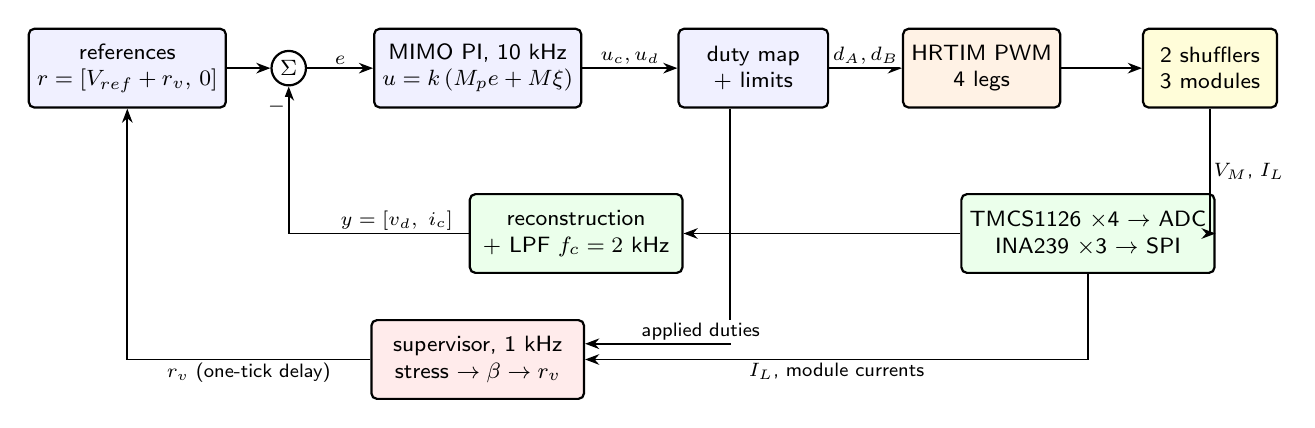
\begin{tikzpicture}[x=1cm,y=1cm,font=\sffamily\footnotesize,
    b/.style={draw,rounded corners=2pt,thick,minimum height=10mm,align=center,inner sep=3pt},
    f/.style={-{Stealth[length=1.8mm]},semithick},
    l/.style={font=\sffamily\scriptsize,fill=white,inner sep=1pt}]
  % forward path
  \node[b,fill=blue!6,minimum width=22mm]  (ref)  at (1.1,0)  {references\\$r = [V_{ref}+r_v,\,0]$};
  \node[draw,circle,thick,inner sep=1.5pt] (sum)  at (3.15,0)  {$\Sigma$};
  \node[b,fill=blue!6,minimum width=25mm]  (pi)   at (5.55,0)  {MIMO PI, 10 kHz\\$u = k\,(M_p e + M\xi)$};
  \node[b,fill=blue!6,minimum width=19mm]  (map)  at (9.05,0)   {duty map\\+ limits};
  \node[b,fill=orange!10,minimum width=19mm] (pwm) at (11.95,0) {HRTIM PWM\\4 legs};
  \node[b,fill=yellow!15,minimum width=17mm] (pl)  at (14.85,0) {2 shufflers\\3 modules};
  % feedback path
  \node[b,fill=green!8,minimum width=27mm]  (sen)  at (13.3,-2.1) {TMCS1126 $\times$4 $\rightarrow$ ADC\\INA239 $\times$3 $\rightarrow$ SPI};
  \node[b,fill=green!8,minimum width=27mm]  (lpf)  at (6.8,-2.1)  {reconstruction\\+ LPF $f_c = 2$ kHz};
  % supervisor
  \node[b,fill=red!8,minimum width=27mm]   (sup)  at (5.55,-3.7)  {supervisor, 1 kHz\\stress $\rightarrow\beta\rightarrow r_v$};
  % wiring
  \draw[f] (ref) -- (sum);
  \draw[f] (sum) -- node[l,above]{$e$} (pi);
  \draw[f] (pi) -- node[l,above]{$u_c, u_d$} (map);
  \draw[f] (map) -- node[l,above]{$d_A, d_B$} (pwm);
  \draw[f] (pwm) -- (pl);
  \draw[f] (pl.south) |- node[l,pos=0.25,right]{$V_M$, $I_L$} (sen.east);
  \draw[f] (sen) -- (lpf);
  \draw[f] (lpf.west) -| node[l,pos=0.2,above]{$y = [v_d,\ i_c]$} node[l,pos=0.93,left]{$-$} (sum.south);
  \draw[f] (sen.south) |- node[l,pos=0.75,below]{$I_L$, module currents} (sup.east);
  \draw[f] ([xshift=-3mm]map.south) |- node[l,pos=0.6,above]{applied duties} ([yshift=2mm]sup.east);
  \draw[f] (sup.west) -| node[l,pos=0.25,below]{$r_v$ (one-tick delay)} (ref.south);
\end{tikzpicture}

  \caption[{Deployed control architecture}]{Deployed control architecture: the 10\,kHz forward path, the measurement feedback, and the 1\,kHz supervisor that sets the voltage-difference references.}
  \label{fig:ctrlloop}
\end{figure}

Every 100\,$\mu$s the control interrupt reconstructs $\vd$ and $\ic$ from the sensors, filters them at 2\,kHz, runs the MIMO PI and maps $\uc$ and $\ud$ to the leg duties $d_A = \tfrac12(1+\uc+\ud)$ and $d_B = \tfrac12(1+\uc-\ud)$, with limits and a slew of 0.01 per tick (\cref{fig:ctrlloop}). Every millisecond the supervisor forms a stress index from the filtered differential currents and the duty excursion, integrates its governor gain $\beta$ and relaxes the voltage-difference references $r_v$, which reach the controller one tick later. The pseudocode for the interrupt, soft-start, supervisor and state machine is in \cref{app:pseudo}.

\begin{figure}[htbp]
  \centering
  % Firmware supervisory state machine (6_RTOS/App/app.c, 100 Hz task).  Print size.
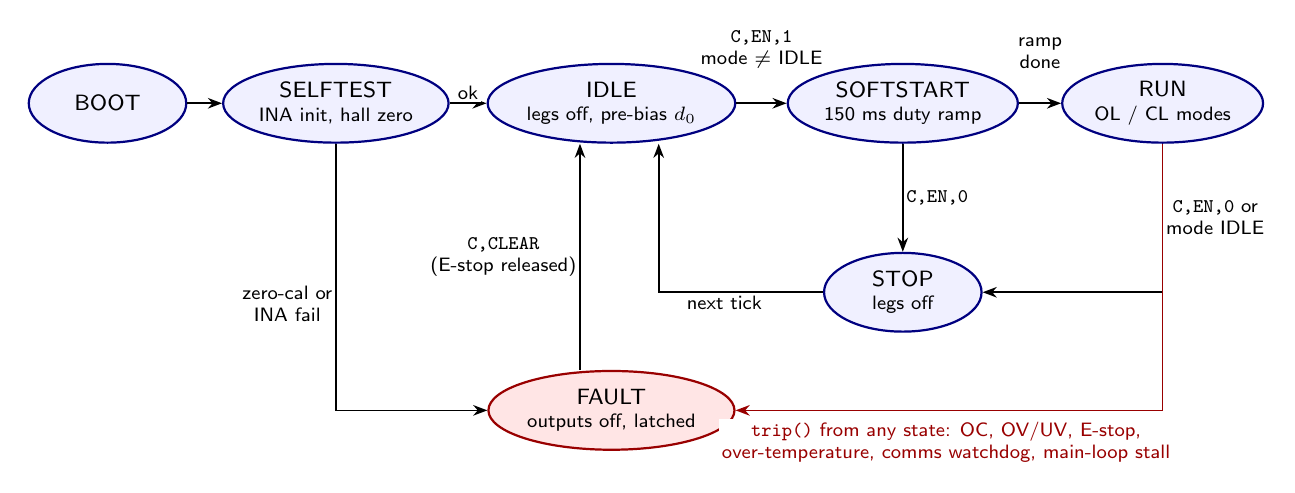
\begin{tikzpicture}[x=1cm,y=1cm,font=\sffamily\footnotesize,
    s/.style={draw,ellipse,thick,draw=blue!50!black,fill=blue!6,minimum width=20mm,minimum height=10mm,align=center,inner sep=1pt},
    sf/.style={s,draw=red!60!black,fill=red!10},
    t/.style={-{Stealth[length=1.8mm]},semithick},
    l/.style={font=\sffamily\scriptsize,fill=white,inner sep=1pt,align=center}]
  \node[s] (boot) at (0.75,0)  {BOOT};
  \node[s] (self) at (3.65,0)  {SELFTEST\\[-1pt]{\scriptsize INA init, hall zero}};
  \node[s] (idle) at (7.15,0)  {IDLE\\[-1pt]{\scriptsize legs off, pre-bias $d_0$}};
  \node[s] (ss)   at (10.85,0) {SOFTSTART\\[-1pt]{\scriptsize 150 ms duty ramp}};
  \node[s] (run)  at (14.15,0) {RUN\\[-1pt]{\scriptsize OL / CL modes}};
  \node[s] (stop) at (10.85,-2.4) {STOP\\[-1pt]{\scriptsize legs off}};
  \node[sf] (flt) at (7.15,-3.9) {FAULT\\[-1pt]{\scriptsize outputs off, latched}};
  \draw[t] (boot) -- (self);
  \draw[t] (self) -- node[l,above]{ok} (idle);
  \draw[t] (idle) -- node[l,above=4mm]{\code{C,EN,1}\\mode $\neq$ IDLE} (ss);
  \draw[t] (ss) -- node[l,above=4mm]{ramp\\done} (run);
  \draw[t] (ss) -- node[l,right]{\code{C,EN,0}} (stop);
  \draw[t] (run) |- node[l,pos=0.25,right]{\code{C,EN,0} or\\mode IDLE} (stop);
  \draw[t] (stop) -| node[l,pos=0.3,below]{next tick} ([xshift=6mm]idle.south);
  \draw[t] (self) |- node[l,pos=0.3,left]{zero-cal or\\INA fail} (flt);
  \draw[t,red!60!black] (run.south) |- (flt.east);
  \node[l,text=red!60!black,anchor=north] at (11.4,-4.0) {\code{trip()} from any state: OC, OV/UV, E-stop,\\over-temperature, comms watchdog, main-loop stall};
  \draw[t] ([xshift=-4mm]flt.north) -- node[l,left]{\code{C,CLEAR}\\(E-stop released)} ([xshift=-4mm]idle.south);
\end{tikzpicture}

  \caption{Supervisory state machine of the firmware (\code{6\_RTOS/App/app.c}, 100\,Hz task).}
  \label{fig:fsm}
\end{figure}

The state machine (\cref{fig:fsm}) starts in BOOT and runs SELFTEST, which initialises the INA239s and zero-calibrates the hall sensors; a failure latches FAULT. From IDLE, an enable command (\code{C,EN,1}) with a non-idle mode starts SOFTSTART, which ramps the duties to their target over 150\,ms before entering RUN. Disabling or selecting IDLE passes through STOP, which turns the legs off, and returns to IDLE on the next tick. Any trip (over-current, over- or under-voltage, E-stop, over-temperature, the communications watchdog or a main-loop stall) switches the outputs off first and latches FAULT, and \code{C,CLEAR} returns to IDLE only once the E-stop is released.
On the Pi, Docker runs InfluxDB and Grafana, \code{pod.py} bridges the serial telemetry and drives the LCD, LED and IR receiver, and \code{eload.py} polls the DL3021 at 5\,Hz and forwards $V_{str}$ to the Nucleo at 2\,Hz (\cref{app:firmware}). The physical signals were checked on the oscilloscope: the dead time and the 180$^\circ$ interleave at 200, 300 and 400\,kHz, and the alignment of the ADC triggers (\cref{fig:scope}).

\subsubsection{Experimental setup and test plan}
\label{sec:setup}
The two set-ups are compared in \cref{tab:setup} and photographed in \cref{fig:setupphotos} (\cref{app:journey}). The tests answer five questions: (i) does the open loop behave as modelled ($V_{M2}/(V_{M2}+V_{M3}) = 1-d$, $\vd = -R_m\im$, a duty-step gain of $-\Vbar$); (ii) does the closed loop regulate ($\vd \rightarrow 0$, $\ic \rightarrow 0$, with the steady-state error and noise measured against $k$ and $\fsw$); (iii) does it reject disturbances (supply and load steps on the bench, shade in the sun); (iv) how much stability margin is there (raising $k$ until the loop misbehaves); and (v) how much energy is returned under shade (delivered against returned power).

\begin{table}[htbp]\centering\small
\caption{Bench and solar experimental set-ups.}
\label{tab:setup}
\begin{tabularx}{\linewidth}{l X X}
\toprule
 & Bench, 16 Oct 2026 (lab) & Solar, 20 Oct 2026 (carpark)\\
\midrule
Modules & R\&S NGE103 three-channel supply \cite{rohde_nge100_ds}, 25\,V set, current limits 0.8 / 1.0 / 1.3\,A & 3 $\times$ KickAss KAUSSP80 \cite{kaussp80_ds}: 80\,W, $V_{oc}$ 25.1\,V, $I_{sc}$ 4.35\,A, $V_{mp} \approx 20.5$\,V\\
Load & Rigol DL3021 \cite{rigol_dl3000_ds} in CV at 70\,V (steps 60--125\,V) & DL3021 in CV at 61\,V ($\approx 3V_{mp}$)\\
Mismatch & supply current limits & cardboard or a shirt over one module\\
Switching frequency & 200, 300, 400\,kHz, one gain set per $\fsw$ & 200\,kHz only\\
Gain scale & per run & sweep $k = 0.1$ to 0.8\\
Instruments & oscilloscope (dead time, interleave) & telemetry and e-load log only\\
Supply for Pi and laptop & mains & battery and inverter\\
Windows & 10 (B01--B09 and B01s, \cref{tab:T1}) & 11, peak sun 15:04--15:13, minimal sun after 15:48\\
\bottomrule
\end{tabularx}
\end{table}
The two set-ups test different things. The supply channels are stiff current limits with no I--V curve and no irradiance, so the bench exercises the loop and the gain set for each switching frequency. The sun exercises the plant the controller was designed for, but only at 200\,kHz and at the irradiance the day gave. The full test matrix is \cref{tab:T1} (21 windows); the pre-flight checklist and power-up order are in the repository (\code{0\_Documentation/experiment\_checklist.md}).

Every metric has one definition for every phase (\code{stepmetrics.py}, \cref{app:synth}).

The hardware cannot resolve the loop dynamics. Telemetry arrives at about 44\,Hz (11--14\,Hz on three 200\,kHz bench runs) while the loop time constants are 1--10\,ms, so hardware rise and settling times are bounds ($\le 23\ms$, one telemetry frame). The hardware does resolve steady-state error, noise, second-scale disturbances, duty-step amplitudes and energy, and the step response is taken from the models.

\subsection{Risks}
\label{sec:risks}
The risk register from the proposal (\cref{tab:risk}, \cref{app:risk}) was kept and updated through the project, and the earlier shuffler's failure (\cref{sec:lit_dpp}) is why protection was designed in from the start rather than added later. Several risks materialised. Scope creep compromised the PCB revisions and features, leaving a single board. Firmware faults were contained by the E-stop, fault latching and state telemetry: faults 0x10 (module under-voltage) and 0x2000 (main-loop stall) tripped three times on 16 Oct when gains were applied live (\cref{tab:T3kscale}), and each time the outputs switched off safely. The averaged model was inaccurate, over-estimating the current-loop gain fivefold, but this was caught in QSPICE before any hardware ran. The top voltage sensor (U10) could not be read and was replaced by the e-load readback. Electrical safety (component ratings and a 15\,A string fuse) and outdoor testing (sun, fire and rain) were managed by procedure, and no risk led to injury or to component damage (U10's isolator was wired backwards at assembly).

\subsection{Ethics}
\label{sec:ethics}
Electrical safety followed QUT's HSE protocols for electrical workspaces: PPE, a 15\,A string fuse, hardware and software E-stops, over-current, over- and under-voltage and over-temperature envelopes in the firmware, and a rule that the system was never left energised unattended. For data security and privacy, all services are hosted locally on the Raspberry Pi with authentication and no cloud connection, only sensed data and internal states are streamed, and credentials are excluded from version control. For integrity, AI assistance (Claude) was used for derivation checking, scripting and the results pipeline; every result can be reproduced from the repository (\code{make all}). 

\subsection{Sustainability}
\label{sec:sustainability}
The project was sustained by constant collaboration (bi-weekly team meetings, a shared GitHub repository and defined hand-over milestones with the hardware teammate). The future of the project is supported by every folder of the repository containing a README, videos recordings expaining the project and regenerable results are all in the repository. Because the shuffler processes only the mismatch power, its component ratings and losses scale with the shading rather than with the string power, which supports more efficient use of existing solar capacity (UN SDG~7.3).

\section{Results, Analysis and Discussion}
\label{sec:results}

% Numbers come from 8_Results/analysis/out (make all); figures from
% tools/make_results_figs.py.

\subsection{Proposed Solution}
\label{sec:solution}
The delivered system (\cref{fig:device}) is a self-contained power shuffler for a three-module string: one Version 0 PCB carrying two interleaved buck-boost shufflers, the NUCLEO-G474RE that closes the loop, and a Raspberry Pi pod with an LCD, an RGB LED and an IR receiver, in a printed enclosure with a heatsink. Against the objectives, the $N$-module averaged model gives the plant and its DC gain in closed form (\cref{sec:analytical}); the decoupling MIMO controller is written once in C and runs unchanged in SIL, in QSPICE and in the firmware; the controller board senses the four winding currents and the module voltages; and the system was validated on the bench and on a real string in the sun. In use, the operator picks a preset with the IR remote or the parameter page, the firmware soft-starts the legs and closes the loop, and the module-voltage differences and circulating currents are held at zero while Grafana shows the live telemetry. Any trip latches FAULT with the legs switched off.

\begin{figure}[htbp]
  \centering
  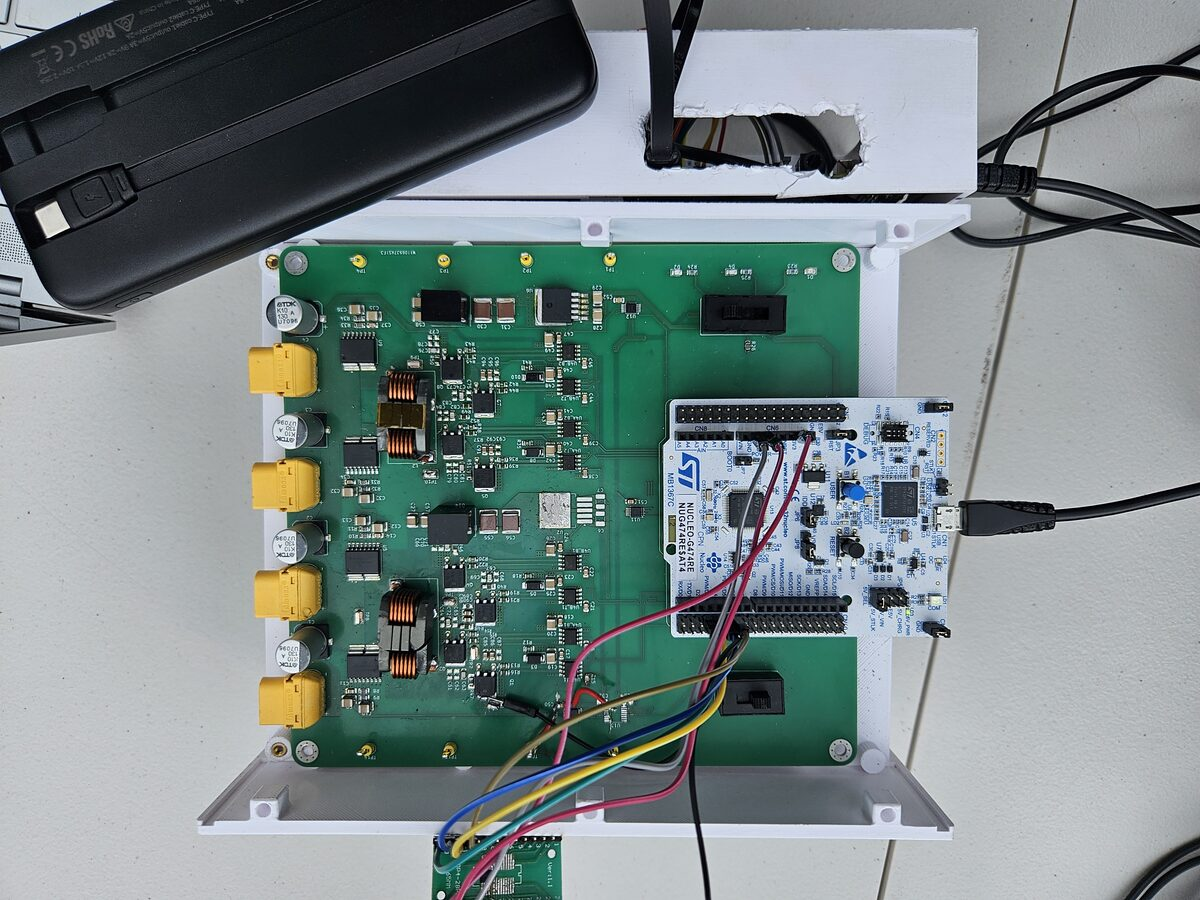
\includegraphics[height=5.0cm]{20261020_112730}
  \caption[{The built power shuffler on 20 Oct 2026}]{The built power shuffler on 20 Oct 2026: PCB, Nucleo, Pi pod, LCD and heatsink (the CAD render is on the title page).}
  \label{fig:device}
\end{figure}

\subsection{Analytical}
\label{sec:res_analytical}
The analytical $N=3$ model sets the expectation for every later phase. \Cref{tab:G} reads its DC gain as what one per cent of duty does. On every plant and in every model, 1\,\% of common-mode duty moves the voltage difference by about 0.4\,V, close to $\Vbar/100$, because $Z_e \gg R_m$ (\cref{sec:analytical}). The current block is where the plants differ. With averaged switches, 1\,\% of differential-mode duty moves the circulating current by 6.7\A; once the switching resistance is included it is 1.4\A{} at 200\,kHz and 0.24\A{} at 400\,kHz. The gain identified in QSPICE on the bench operating point (1.43 / 1.39\A) sits within 13\,\% of the analytical bench value (1.61\A), which is the evidence that $R_{sw}$ is real. The averaged Simulink plant over-estimated the current-loop gain fivefold (7.42\A), and its gain set was rejected for the hardware. The last column of \cref{tab:G} is the one term the averaged model cannot predict: a 0.14--0.25\V{} cross-coupling from differential-mode duty into $\vd{}_{,1}$, caused by the dead time, which the identified gain matrix cancels.

% generated by tools/make_tables.py -- do not edit by hand
\begin{table}[htbp]\centering
\footnotesize
\caption[{DC gain matrix $G(N)$ read as ``what 1\,\% of duty does''}]{DC gain matrix $G(N)$ read as ``what 1\,\% of duty does'': the voltage block (common-mode duty $u_c$ to the voltage difference $v_d$) and the current block (differential-mode duty $u_d$ to the circulating current $i_c$), shuffler 1 / shuffler 2 where they differ. The last column is the dead-time cross-coupling that only the switching model shows. The gain sets store $M = G^{-1}\mathrm{diag}(k_I)$, so $G = \mathrm{diag}(k_I)\,M^{-1}$.}\label{tab:G}
\begin{tabular}{l l r r r}
\toprule
Obtained from & Plant & \makecell[r]{$\Delta v_d$ [V] per\\1\,\% of $u_c$} & \makecell[r]{$\Delta i_c$ [A] per\\1\,\% of $u_d$} & \makecell[r]{cross: $\Delta v_{d1}$ [V]\\per 1\,\% of $u_{d1}$} \\
\midrule
Analytical & Solar string, averaged switches ($R = 61$\,m$\Omega$) & -0.40 & 6.72 & 0.00 \\
Analytical & Solar string, 200\,kHz ($R_{sw} = 0.29\,\Omega$) & -0.38 & 1.41 & 0.00 \\
Analytical & Solar string, 400\,kHz ($R_{sw} = 1.72\,\Omega$) & -0.29 & 0.24 & 0.00 \\
Analytical & Bench supplies in current limit, 200\,kHz & -0.47 & 1.61 & 0.00 \\
Simulink step tests & Bench, averaged switches (rejected) & -0.46 / -0.47 & 7.42 / 7.42 & -0.01 \\
QSPICE step tests & Bench, 200\,kHz (deployed) & -0.46 / -0.47 & 1.43 / 1.39 & -0.25 \\
QSPICE step tests & Bench, 300\,kHz (deployed) & -0.45 & 0.59 / 0.57 & -0.17 \\
QSPICE step tests & Bench, 400\,kHz (deployed) & -0.42 / -0.43 & 0.23 & -0.14 \\
\bottomrule
\end{tabular}
\end{table}


The root locus (\cref{fig:ana_rl}, \cref{app:analytical}) shows the margin of the deployed gains. With the deployed $M$, the voltage-loop poles stay real up to $k \approx 1$ and the circulating-current loops become complex first. The same $M$ on the 61\,m$\Omega$ averaged plant crosses into the right half-plane near $k \approx 1.5$, a second reason the averaged gain set could not be used. The open-loop phase portraits (\cref{fig:ana_portraits}) show the same trend: as the plant resistance grows with $\fsw$, the voltage mode changes from a lightly damped focus to an over-damped node.
\subsection{Simulink}
\label{sec:res_simulink}
The MIL model passed all seven validation tests (\cref{tab:validate}, \cref{app:simulink}). \Cref{fig:twin_sim} shows the carpark twin, which adds the sensing model, closing the loop on the three-module solar plant. In (a) a $+1\V$ step on the $\vd{}_{,2}$ reference is followed with the first-order shape of the design, with $\tau$ of 11.6, 3.5 and 0.56\ms{} at $k = 0.1$, 0.3 and 1 against the design 10.6, 3.5 and 1.06\,ms, while $\vd{}_{,1}$ does not move: the voltage loops are decoupled. In (b) and (c) module 3 loses a third of its irradiance. In open loop at $D = 0.5$ the shufflers already carry most of the deficit but leave a residual $\vd = -R_m\im$ of 0.06 and 0.12\V; the closed loop removes it within 15\ms{} at $k = 0.3$. Panel (c) shows why the string recovers: the shuffled currents step to 0.97 and 1.92\A, the weighted sums of the mismatch predicted by $T^{-1}\delta I$ (0.96 and 1.92\,A), and the string current settles at the mean module current, 3.82\A. The only overshoot in the twin is on the bench plant at $k=1$ (8.8\,\%).

\begin{figure}[htbp]
  \centering
  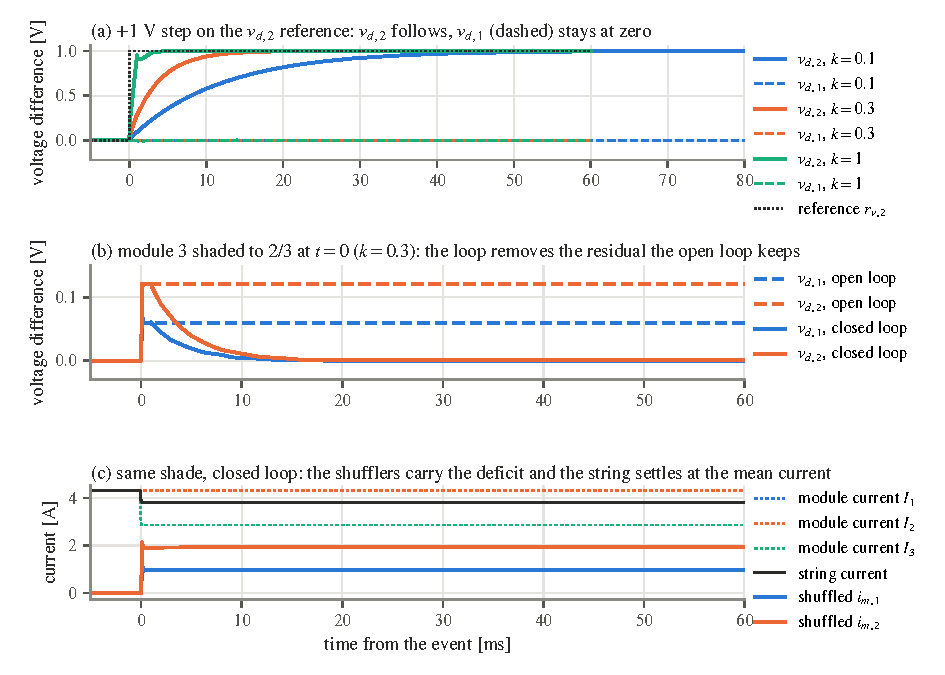
\includegraphics[width=\linewidth]{results/twin_sim}
  \caption[{Simulink carpark twin (averaged switches, sensing model, solar plant)}]{Simulink carpark twin (averaged switches, sensing model, solar plant): (a) $+1\V$ reference step at three gain scales, (b, c) module 3 shaded to two thirds at $t=0$, closed loop against open loop.}
  \label{fig:twin_sim}
\end{figure}

\subsection{QSPICE}
\label{sec:res_qspice}
\Cref{fig:qspice_run} is the strongest simulated evidence, because it runs the unchanged firmware control core as a DLL against real switches, drivers, dead time and the sensor models. A single run at $k = 0.3$ on the solar plant closes the loop on the open-loop residual, follows a $+1\V$ step on the $\vd{}_{,2}$ reference with $\vd{}_{,1}$ held, and then rejects a shade on module 3. The shuffled currents pick up the mismatch, the circulating currents stay within $\pm0.1\A$, and the string current falls to the mean module current.

\begin{figure}[htbp]
  \centering
  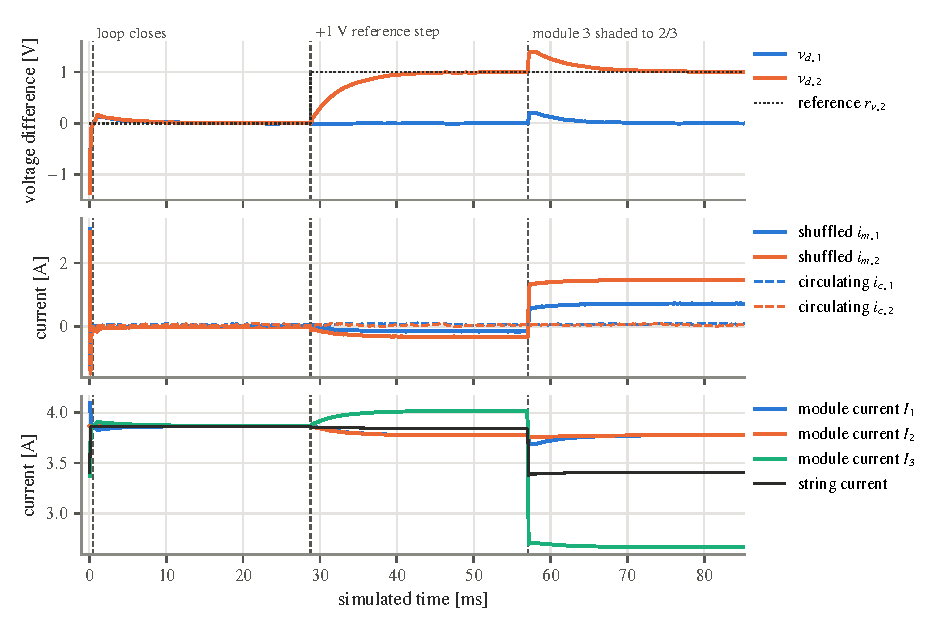
\includegraphics[width=\linewidth]{results/qspice_run}
  \caption[{QSPICE switching model with the firmware control DLL, solar plant, $k=0.3$}]{QSPICE switching model with the firmware control DLL, solar plant, $k=0.3$ (100\,$\mu$s bin means of the switching waveforms): loop closure, $+1\V$ reference step on $\vd{}_{,2}$, then module 3 shaded to two thirds.}
  \label{fig:qspice_run}
\end{figure}

The 200\,kHz gain matrix identified from this model, and deployed on the hardware, is
\begin{equation}
  G_{200} \;=\;
  \begin{array}{r@{\;}c}
   & \begin{array}{rrrr} \;\;u_{c1} & \;\;u_{c2} & \;\;u_{d1} & \;\;u_{d2} \end{array}\\[2pt]
  \begin{array}{r} v_{d1}\\ v_{d2}\\ i_{c1}\\ i_{c2} \end{array} &
  \left[\begin{array}{rrrr} -46.3 & -0.2 & -24.7 & -0.1\\ -0.2 & -46.9 & -0.1 & -27.4\\ -1.1 & -0.3 & 142.5 & 1.4\\ -1.4 & -0.9 & 0.1 & 139.0 \end{array}\right]
  \end{array}
  \label{eq:G200}
\end{equation}
in volts or amperes per unit duty. Its structure is the analytical one: a voltage block of $-\Vbar \approx -46.6\V$ with neighbour terms below 0.5\,\%, a current block of $\Vbar/R_c$, and almost no current response to the common-mode duty. The only new terms are the $\vd/\ud$ cross terms of $-25$ and $-27\V$, the dead-time effect. The matrix is well conditioned (cond$\,G = 3.2$), so its inverse, the stored gain matrix $M$, is well behaved (\cref{app:gains}).

The device model also reproduces the switching ripple (\cref{tab:T6}). QSPICE matches $\Delta\ic = \Vbar/(2\fsw(L+M))$ to within 1--3\,\% at all three frequencies. Each winding carries half of the circulating ripple, and in the shuffled current the two interleaved windings cancel, leaving only 0.2--0.4\,A. Had the circulating mode seen $L-M$ instead, the ripple would be 28--57\,A, so this result also confirms the as-built anti-series coupling. The telemetry cannot see the ripple: its samples are box-averaged over a whole control tick, and their spread is sensing noise. QSPICE was not used to judge milliamp and millivolt levels of $\ic$ and $\vd$, which depend on milliohm parasitics and nanosecond edges.

% generated by tools/make_tables.py -- do not edit by hand
\begin{table}[htbp]\centering
\small
\caption[{Peak-to-peak switching ripple: analytical against QSPICE}]{Peak-to-peak switching ripple in A. The circulating mode sees $L+M$, so the analytical law is $\Delta i_c = \bar V/(2 f_{sw}(L+M))$ with $L+M = 13.75\,\mu$H and $\bar V = 46.6$\,V. Each winding carries half of it ($\Delta i_A$); in the shuffled current the two interleaved windings cancel ($\Delta i_m$). The 44\,Hz telemetry cannot see the ripple: its $\sigma(i_c)$ is sensing noise.}\label{tab:T6}
\begin{tabular}{r r r r r r r}
\toprule
$f_{sw}$ [kHz] & \makecell[r]{$\Delta i_c$\\analytical} & \makecell[r]{$\Delta i_c$\\QSPICE} & \makecell[r]{$\Delta i_A$ per\\winding} & \makecell[r]{$\Delta i_m$\\QSPICE} & \makecell[r]{QSPICE vs\\analytical} & \makecell[r]{telemetry\\$\sigma(i_c)$} \\
\midrule
200 & 8.47 & 8.39 & 4.25 & 0.19 & -1\,\% & 0.30 \\
300 & 5.65 & 5.58 & 2.85 & 0.20 & -1\,\% & 0.05 \\
400 & 4.24 & 4.09 & 2.18 & 0.39 & -3\,\% & 0.08 \\
\bottomrule
\end{tabular}
\end{table}


\subsection{Bench Testing}
\label{sec:bench}
Bench testing was a success. The set-up was the three-channel supply (NGE103), the electronic load (DL3021), an oscilloscope, a laptop and the full system (\cref{tab:setup}). Testing started at 200\,kHz in open loop to get the baseline behaviour, then closed the loop at 0.1, 0.2 and 0.3 of the QSPICE gains, then ran 300\,kHz at 0.3 and 0.5 and 400\,kHz at 0.3. 300\,kHz was the most favourable: as the switching frequency rises the open-loop residual and the current-loop gain fall, but the heatsink temperature rises (\cref{app:thermal}). An open-loop test at 100\,kHz was also explored on 13 Oct; the system ran, but with erratic behaviour. The supplies cannot deliver as much as the panels, so the bench exercised the loop rather than the power stage.

\textbf{Open loop.} The three open-loop duty steps (\cref{fig:S5}, \cref{tab:T3duty} in \cref{app:bench}) confirm the model's DC gain on hardware: every measured change in $\vd$ is within 0.02\,V of $-\Vbar\Delta\uc$, and the shuffler whose duty did not change stays put. At duties of 0.5 the residual $\vd{}_{,2}$ is $-0.17\V$ at 200\,kHz, $-0.58\V$ at 300\,kHz and $-0.94\V$ at 400\,kHz (\cref{tab:T2ol}). This is the $-R_m\im$ drop, growing with $R_{sw}$, that the closed loop has to remove.


\begin{figure}[htbp]
  \centering
  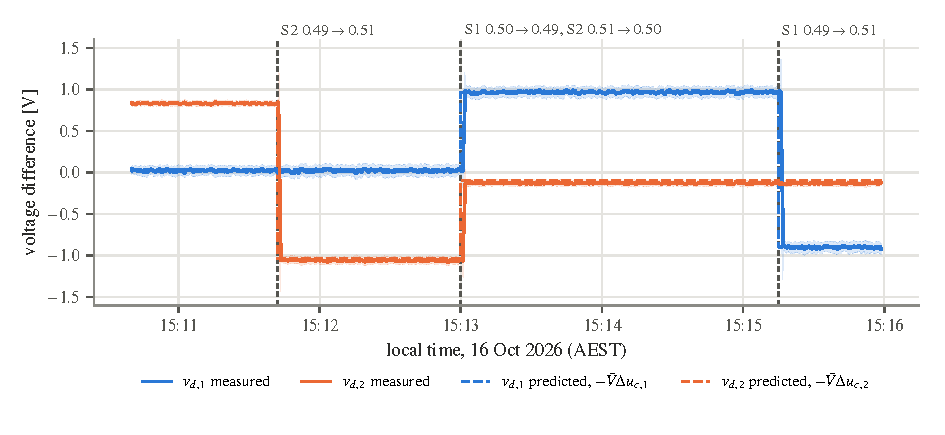
\includegraphics[width=\linewidth]{results/duty_steps}
  \caption[{Open-loop duty steps on the bench (16 Oct, 200\,kHz)}]{Open-loop duty steps on the bench (16 Oct, 200\,kHz): measured voltage differences (1\,s mean, $\pm1\sigma$ band) against the averaged-model prediction $-\Vbar\Delta\uc$ (dashed), which overlays the measurement.}
  \label{fig:S5}
\end{figure}

\textbf{Closed loop.} \Cref{fig:B06} shows 300\,kHz at $k = 0.3$ through seven step changes of the supply channels. The shuffled currents move to carry each new mismatch while the 1\,s means of both voltage differences stay within $\pm0.008\V$ and of both circulating currents within $\pm0.03\A$; the raw samples scatter by 0.016\V{} and 0.055\A. Over all 22 settled closed-loop segments, $|\bar v_{d,2}| \le 0.010\V$ and $|\bar\imath_{c,2}| \le 0.066\A$, with sample noise $\sigma(\vd{}_{,2})$ of 0.013--0.17\V{} (\cref{tab:T2cl}): the references are held with no measurable offset, and the residual is sensing noise. The 150\,ms soft-start leaves 0--0.8\,V on $\vd{}_{,2}$, which the loop removes within one telemetry frame in 10 of 23 closures and within 3\,s, limited by noise, in the rest (\cref{tab:T3close}).

\begin{figure}[htbp]
  \centering
  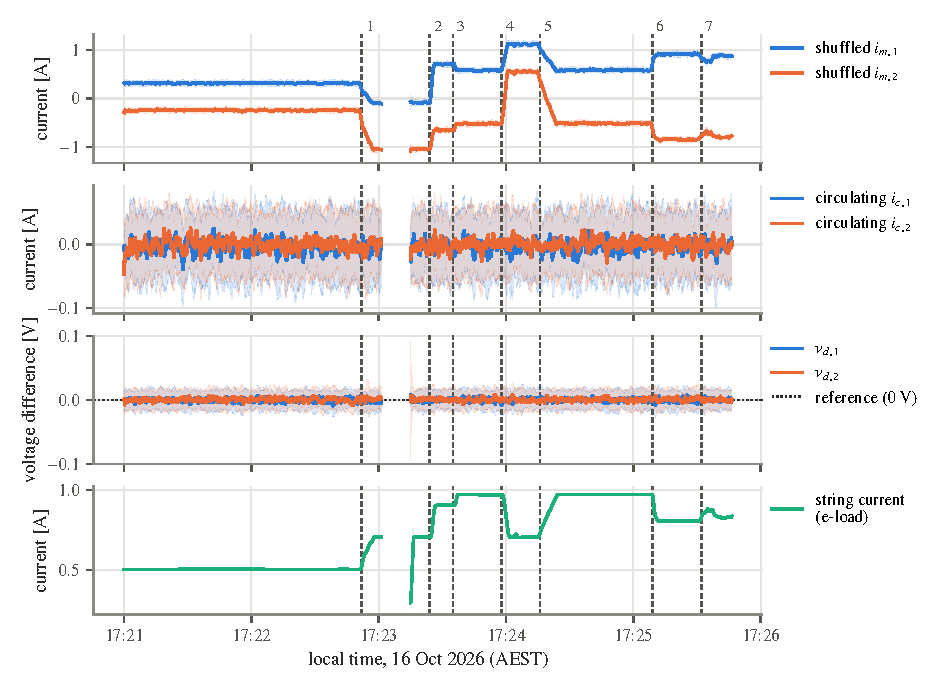
\includegraphics[width=\linewidth]{results/bench_B06}
  \caption[{Bench, 300\,kHz closed loop, $k=0.3$ (B06)}]{Bench, 300\,kHz closed loop, $k=0.3$ (B06): 1\,s means with the $\pm1\sigma$ spread of the 44\,Hz samples. The dashed lines 1--7 are step changes of the supply channels; the shuffled currents move, the voltage differences and circulating currents do not.}
  \label{fig:B06}
\end{figure}

\textbf{Stability limit and faults.} At 300\,kHz and $k = 0.6$ the loop oscillated ($\sigma(\vd{}_{,2}) = 1.41\V$, 11.8\,V peak to peak) for 6\,s before it was stopped, so the 300\,kHz gain set loses margin above $k \approx 0.5$. Applying a new gain scale while the loop was running tripped the firmware three times (\cref{tab:T3kscale}): once on module under-voltage and twice on a main-loop stall. Each trip switched the legs off and latched FAULT as designed, but gains should be set before the loop is closed. Three 200\,kHz runs (B02--B04) logged at only 11--14\,Hz, so every time metric there is a bound of at least 70\,ms.

\textbf{Limitations.} The board carries only two shufflers, and boards cannot be stacked, so scalability cannot be tested. The two shufflers are hard-wired together and cannot be driven independently. The top INA239 does not work, so $V_{M1}$ is inferred from the e-load. And a change of switching frequency needs a new identification and gain set.

\subsection{Solar Test}
\label{sec:solar}
Solar testing was also a success: eleven windows and 36\,min of run time, with the loop closed from $k = 0.1$ to 0.8 without a fault (\cref{tab:T1}). \Cref{fig:S02} shows the peak-sun window at $k = 0.1$. As the sun came out and the mismatch grew, the shuffled currents swung to $-3.3$ and $-1.5\A$ while the 1\,s means of the voltage differences stayed within $\pm0.06\V$. The open-loop residual of the same afternoon ($-0.32\V$ at peak sun, $-0.07\V$ in minimal sun) was removed in closed loop. During the shade events the current mismatch changed by 0.5--1.5\,A over 2--6\,s, $\vd{}_{,2}$ deviated by less than 0.3\,V and recovered, and the duties never left 0.45--0.55, far from their limits (\cref{tab:T3shade}).

\begin{figure}[htbp]
  \centering
  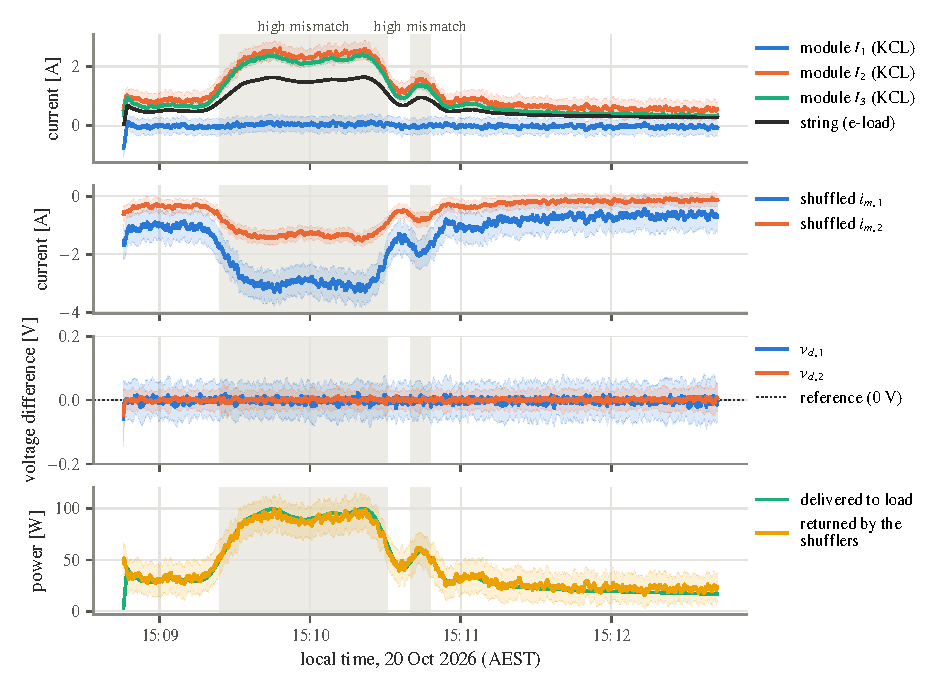
\includegraphics[width=\linewidth]{results/solar_S02}
  \caption[{Carpark string at peak sun, 200\,kHz closed loop, $k=0.1$ (S02, 20 Oct 2026)}]{Carpark string at peak sun, 200\,kHz closed loop, $k=0.1$ (S02, 20 Oct 2026): module currents rebuilt by KCL, shuffled currents, voltage differences and the power delivered to the 61\,V load and returned by the shufflers (1\,s means, $\pm1\sigma$ bands; shaded spans are the detected high-mismatch periods).}
  \label{fig:S02}
\end{figure}

The top module was shaded to almost zero current (a shirt over about a third of the panel): by KCL it carried $\approx 0\A$ in every solar window, while modules 2 and 3 carried up to 2.5\,A. The string current settled at the mean module current, as the model predicts, so the shufflers delivered the other two modules' power to the 61\,V load, up to 99\W{} during S02. A plain series string could not have supplied that load at all, so the energy returned equals the energy delivered: $E_{ret} = 10.6\Wh \approx E_{load}$ over the 36\,min (\cref{tab:T7solar}). \note{Confirm what happened to module 1 and phrase the energy return accordingly.} The measured ratio $E_{load}/E_{modules}$ of 99.2--100\,\% closes by construction, because $V_{M1}$ comes from the e-load and the module currents from KCL, so it is not a converter efficiency.

The weather was the main limitation. After 15:48 the sun was minimal ($P_{load}$ 2--13\,W), which allowed the gain sweep but not enough mismatch power to stress the loop. The closed-loop response to panel dynamics is therefore validated at low power, and otherwise rests on the models.

\subsection{Synthesising Results}
\label{sec:synthesis}
\Cref{fig:metrics} (and \cref{tab:T5s4}, \cref{app:synth}) compare the $+1\V$ reference step across the three models. The fitted time constant follows the design $1/(k\,2\pi\,150)$ at every gain scale: within 0.86--1.22$\times$ in the analytical model, 0.52--1.17$\times$ in QSPICE and 0.38--1.10$\times$ in the Simulink twin. The models drift faster than the design at high $k$, where the plant's own dynamics add to the integrator. Every one of these time constants is shorter than one 23\,ms telemetry frame, so the hardware cannot resolve the step response. What it does resolve agrees with the models: the DC gain (open-loop duty steps), zero steady-state error, a noise-limited residual, and closures within one frame.

\begin{figure}[htbp]
  \centering
  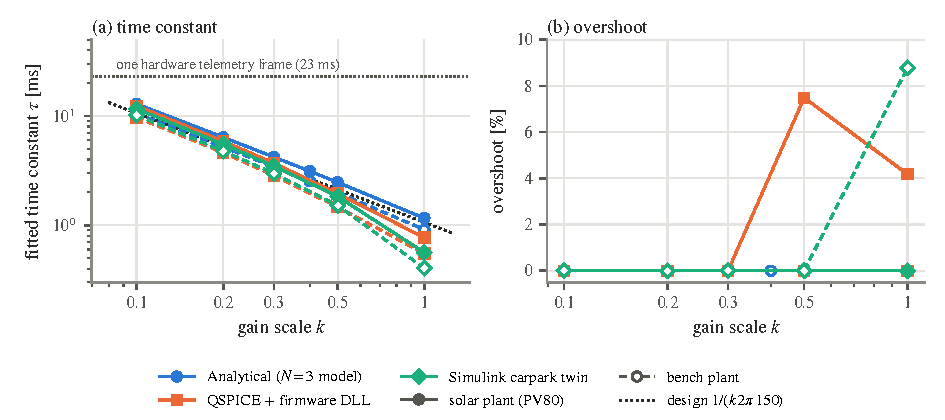
\includegraphics[width=\linewidth]{results/metrics_k}
  \caption[{$+1\V$ reference step on $\vd{}_{,2}$ (200\,kHz gain set) against gain scale}]{$+1\V$ reference step on $\vd{}_{,2}$ (200\,kHz gain set) against gain scale: (a) fitted time constant, with the first-order design and one hardware telemetry frame; (b) overshoot. Filled markers and solid lines are the solar plant, hollow markers and dashed lines the bench plant.}
  \label{fig:metrics}
\end{figure}


Most of the overshoot entries are zero (\cref{fig:metrics}(b), \cref{tab:T5s4}), and that is the design working rather than missing data. Because the controller inverts the DC gain, $MG$ is diagonal and each loop is an integrator acting on a plant of unit DC gain, which is a first-order closed loop, and a first-order response cannot overshoot. Overshoot needs the dynamics the design neglects: the 2\,kHz measurement filter, the one-tick delay of the 100\,$\mu$s sampling, and the plant's LC modes. These only matter once the loop's time constant falls to a few times their 0.1--0.3\,ms. That happens at $k \ge 0.5$ ($\tau \le 2\ms$), where QSPICE shows 7.5\,\% at $k = 0.5$ and 4.2\,\% at $k = 1$ on the solar plant and the Simulink twin 8.8\,\% on the bench plant at $k = 1$. The analytical model includes the filter but not the sampling delay, so it never overshoots.

Together these results support the gap claim: the same gain matrix decouples the voltage and current loops in an averaged model, in a switching model with sensing quantisation and dead time, and on the board at three switching frequencies. Where the phases disagree there is a reason. The Simulink twin is faster than the design at $k \ge 0.5$ because its averaged plant has no $R_{sw}$. QSPICE overshoots at high $k$ through the sampling delay and the filter. And the 300\,kHz gain set, identified at the bench operating point, loses margin on hardware earlier than the models suggest ($k = 0.6$ oscillation).

The risk, ethics and sustainability outcomes were met. There was no injury and no damaged component; U10's isolator was wired backwards before any testing. Every fault was latched by the firmware, all data stayed local on the Pi, and the string returned 10.6\Wh{} with one module producing nothing. The supervisor's feedback to push the controller algorithms into QSPICE, start rapidly testing early on in either simulink / qspice, support of learning from textbooks and papers and a strong emphasis on safety shaped the methods and direction of the project.

\section{Conclusion}
\label{sec:conclusion}
% Your version: 07_conclusion_draft.tex (future work and recommendations kept).

This project asked how the coupled dynamics of several interleaved buck-boost power shufflers in one string can be modelled and controlled. The answer is the $N$-module averaged model. It splits each shuffler into a shuffled mode and a circulating mode, and it gives the string's DC gain in closed form, $\vd \approx -\Vbar\uc$ and $\ic = (\Vbar/R_c)\ud$, with neighbour coupling below one per cent. Inverting that gain gives a decoupling integral controller on $[\vd, \ic]$: it commands the shuffled currents so the string equalises, and a partially shaded string reaches its maximum power point when the module voltages are equal, which the loop enforces.

The controller was carried from the analytical model through Simulink and QSPICE to the firmware, as one C core and one results pipeline, and validated on the bench and in the sun. On hardware it holds the module-voltage differences within $\pm0.010\V$ and the circulating currents within $\pm0.07\A$, limited by sensing noise. Its bandwidth follows the design $\tau = 1/(k\,2\pi\,150)$ to within the spread of the three simulations (0.4--1.2$\times$). Across 21 test windows on two days the loop closed from $k=0.1$ to 0.8 in the sun without a fault. The only instability was deliberately provoked ($k = 0.6$ at 300\,kHz), and the only trips came from live gain changes. With the top panel shaded to almost zero current, the shufflers delivered up to 99\W{} and 10.6\Wh{} over the afternoon to a 61\,V load that a plain series string could not have supplied. The averaged model's one real error, a fivefold over-estimate of the current-loop gain, was traced to a switching resistance $R_{sw} = 64\,C_p\fsw^3(L+M)^2$ and caught in QSPICE before any hardware ran. The result is a complete, reproducible system and a starting point for further work on MIMO control of DPP strings.

\textbf{Future work.} Scalability comes first: determine how the relationships change when more shufflers act in one string, or when a shuffler handles a varying number of panels, which needs boards that can be chained and driven independently. The gain calculation for a new switching frequency can now be streamlined, since $R_{sw}(\fsw)$ is a formula. Other controllers should be generated and compared against this one (LQR, MPC, an observer-based design, and the extended-Kalman-filter approach of \cite{kabalci_highly_2022}), as should a cost-function or machine-learning search for optimal gains. The firmware should move from its superloop to a real-time operating system, as FreeRTOS was planned, so that the control, sensing, safety and telemetry tasks are scheduled with explicit priorities and deadlines. Three firmware items were found in testing: refuse \code{C,APPLY} while the loop is running, add the COMP/DAC hardware over-current trip, and rework U10's isolator. Further work should also test other panel arrangements and dynamic configurations, and applications outside solar (mining, computing, industrial power and batteries), including whether the technology would win a solar car race.

\textbf{Recommendations.} The most immediate work is more data: stress-test the system on a very sunny day with every panel connected. To measure efficiency properly, add an MPPT algorithm, run it on the Raspberry Pi, which already controls the load over USB, and keep the load's limits in mind if the same set-up is reused. The electrical safety limits restrict which experiments can be run, so they should be designed around from the start. The system favours high switching frequencies, so GaN devices are worth revisiting. Mechanically, downsize the heatsink, improve the fasteners, reconfigure the PCB and redesign the enclosure, and consider consolidating the microcontroller and the microcomputer onto one board. Finally, hands-on development was the fastest route to understanding: anyone continuing the project should start from the GitHub repository, its manufacturing notes and its user guides.


\clearpage
\IfFileExists{IEEEtran.bst}{\bibliographystyle{IEEEtran}}{\bibliographystyle{ieeetr}}
\bibliography{refs}

\clearpage
\appendix
\sloppy
\section{Research Project Timeline}
\label{app:timeline}

\begin{figure}[htbp]
  \centering
  \resizebox{\linewidth}{!}{% Two-semester timeline (weeks) with milestones; simple Gantt drawn in TikZ
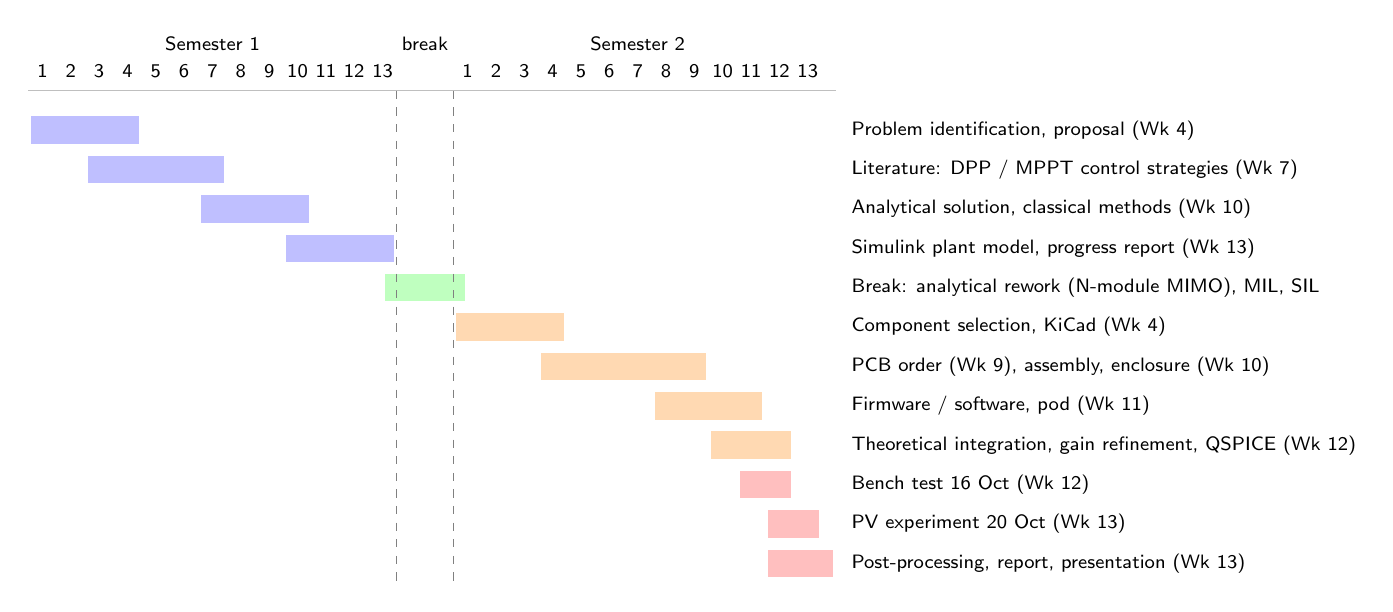
\begin{tikzpicture}[x=0.36cm,y=0.5cm,font=\sffamily\scriptsize]
  % axes: semester 1 weeks 1-13, break, semester 2 weeks 1-13
  \foreach \w in {1,...,13}{\node at (\w,0.5) {\w};}
  \node at (7,1.2) {Semester 1};
  \foreach \w in {1,...,13}{\node at (\w+15,0.5) {\w};}
  \node at (22,1.2) {Semester 2};
  \node at (14.5,1.2) {break};
  \draw[gray!50] (0.5,0) -- (29,0);
  \newcommand{\gbar}[5]{\fill[#5] (#1-0.4,-#3*1.0-0.35) rectangle (#2+0.4,-#3*1.0+0.35); \node[anchor=west] at (29.2,-#3) {#4};}
  \gbar{1}{4}{1}{Problem identification, proposal (Wk 4)}{blue!25}
  \gbar{3}{7}{2}{Literature: DPP / MPPT control strategies (Wk 7)}{blue!25}
  \gbar{7}{10}{3}{Analytical solution, classical methods (Wk 10)}{blue!25}
  \gbar{10}{13}{4}{Simulink plant model, progress report (Wk 13)}{blue!25}
  \gbar{13.5}{15.5}{5}{Break: analytical rework (N-module MIMO), MIL, SIL}{green!25}
  \gbar{16}{19}{6}{Component selection, KiCad (Wk 4)}{orange!30}
  \gbar{19}{24}{7}{PCB order (Wk 9), assembly, enclosure (Wk 10)}{orange!30}
  \gbar{23}{26}{8}{Firmware / software, pod (Wk 11)}{orange!30}
  \gbar{25}{27}{9}{Theoretical integration, gain refinement, QSPICE (Wk 12)}{orange!30}
  \gbar{26}{27}{10}{Bench test 16 Oct (Wk 12)}{red!25}
  \gbar{27}{28}{11}{PV experiment 20 Oct (Wk 13)}{red!25}
  \gbar{27}{28.5}{12}{Post-processing, report, presentation (Wk 13)}{red!25}
  \draw[dashed,gray] (13.5,0) -- (13.5,-12.5);
  \draw[dashed,gray] (15.5,0) -- (15.5,-12.5);
\end{tikzpicture}
}
  \caption{Project timeline across the two semesters (teaching weeks) with the milestone week of each phase.}
  \label{fig:timeline}
\end{figure}

\begin{table}[htbp]\centering\small
\caption{Development phases and their V-model counterpart.}
\label{tab:phases}
\begin{tabular}{c l l l}
\toprule
Phase & Pipeline & V-model & Primary artefact\\
\midrule
0 & Background research & Concept of operations & proposal, literature review\\
1 & Analytical solution & System requirements & \code{nstring.py}, notebooks, \cref{app:analytical}\\
2 & Model-in-the-loop & High-level design & \code{power\_shuffler\_sim.slx} (4 modules)\\
3 & Component selection & Detailed design & KiCad Version 0 PCB, BOM\\
4 & Firmware / software & Development & \code{6\_RTOS} (C), \code{7\_Pi} (Python, Docker)\\
5 & Software-in-the-loop & Unit verification & C Caller blocks, golden replay\\
6 & QSPICE integration & Subsystem verification & QSPICE integrated model + control DLL\\
7 & Bench test & System verification & 16 Oct 2026, 10 windows (\cref{tab:T1})\\
8 & Solar test, partial shade & System validation & 20 Oct 2026, 11 windows (\cref{tab:T1})\\
9 & Post-processing / synthesis & Acceptance & \code{8\_Results/analysis} (\code{make all})\\
\bottomrule
\end{tabular}
\end{table}

\begin{table}[htbp]\centering\small
\caption{Milestones and progress achieved (proposal $\rightarrow$ progress report $\rightarrow$ delivery).}
\label{tab:timeline}
\begin{tabular}{l l l p{6.2cm}}
\toprule
Semester & Week & Milestone & Progress / change\\
\midrule
1 & 4 & Problem identification, proposal & Research question, objectives, risk register, Gantt (34 weeks)\\
1 & 7 & Existing DPP / MPPT control strategies & Literature review (Appendix A of the proposal), gap statement\\
1 & 10 & Analytical solution using classical methods & Single-shuffler averaged model, equilibrium, linearisation, cascaded PI; marginal stability found\\
1 & 13 & Simulink plant model & 4-module PV string, P--V validation, inner current loop attempt (instability under shade)\\
Break & -- & Analytical rework, MIL, SIL & MIMO reformulation (LQR + integral, then decoupling PI), $N$-module string model, MIL 7-test suite, SIL C core + golden replay\\
2 & 4 & Component selection & STM32G474 Nucleo, TMCS1126, INA239, Raspberry Pi 4B; KiCad Version 0\\
2 & 9 & PCB order & PCBWay board + stencil, components, reflow\\
2 & 10 & Enclosure development & Enclosure, heatsink, pod wiring (IR, LCD, LED, DS18B20)\\
2 & 11 & Firmware / software & Bare-metal C application, control core, telemetry contract, Pi stack (Docker InfluxDB + Grafana)\\
2 & 12 & Theoretical integration / gain refinement & QSPICE integrated model with the control DLL; gain sets per $\fsw$; $R_{sw}$ identified\\
2 & 12 & Bench test & 16 Oct 2026: 200/300/400\,kHz, open and closed loop (\cref{tab:T1})\\
2 & 13 & PV experiment & 20 Oct 2026: 3 $\times$ KAUSSP80 in the carpark, $k=0.1\ldots0.8$\\
2 & 13 & Post-processing & Results pipeline (\code{make all}), REPORT.md, this report, presentation\\
\bottomrule
\end{tabular}
\end{table}

Three things changed from the proposal. The first PCB moved from Semester~1 Week~10 into Semester~2 (progress report, Appendix~A), and the planned Version~1 and Version~2 boards collapsed into a single Version~0 board, which meant compromising on PCB revisions and features. String MPPT integration was deferred, because the electronic load performs it. Interim milestones were reviewed weekly with the supervisor.

\section{Risk Register}
\label{app:risk}
Likelihood and consequence are rated Low (L), Medium (M), High (H) or Critical (C); the overall rating is the higher of the two. The register is the proposal's, with a \emph{Status} column recording what happened.

\begin{landscape}
\begin{longtable}{c p{3.0cm} l c c c p{6.4cm} p{6.2cm}}
\caption{Project risk register with outcome.}\label{tab:risk}\\
\toprule
\# & Risk & Category & L & C & Rating & Mitigation / monitoring & Status at delivery\\
\midrule\endfirsthead
\toprule
\# & Risk & Category & L & C & Rating & Mitigation / monitoring & Status at delivery\\
\midrule\endhead
\bottomrule\endfoot
1 & Scope creep & Project & H & H & H & Strict change control; new requirements deferred to the next revision; supervisor sign-off for additions & Materialised: one PCB revision only, MPPT deferred to the load, features compromised (slide: ``had to compromise on PCB revisions and features'')\\
2 & No PV hardware available & Resource & M & C & H & Procure panels early; fallback QSPICE validation & Mitigated: 3 $\times$ KAUSSP80 80\,W panels, DL3021 load; EcoFlow not used ($V_{oc}$ 75\,V $>$ 60\,V input)\\
3 & Electronics failure & Hardware & M & H & H & Overload protection; spares; one-month buffer & Partly: U10 (top INA239) unusable (isolator wired reversed); worked around with $V_{M1}$ from the e-load\\
4 & Firmware failure & Control sys. & M & H & H & Simulation first (SIL, QSPICE DLL); unit tests; fault latching & Materialised in a contained way: 3 trips on live gain changes (UV, main-loop stall), all latched safely; E-stop and state telemetry worked\\
5 & Monitoring software inaccuracy & Software & L & M & L & Sensor noise filtering; cross-validate against known points & Telemetry at 44\,Hz is noise-limited; rise/settle reported as bounds; B02--B04 logged at 11--14\,Hz\\
6 & Data loss & Data & L & H & M & GitHub, OneDrive, local backups & No loss; every window re-exportable from InfluxDB\\
7 & Unable to access data & Data & L & M & L & Shared cloud repositories, two admins & OK\\
8 & Electrical hazard (50\,V DC class) & Safety & M & C & C & QUT HSE protocols, PPE, isolation, formal risk assessment & No incident; 15\,A fuse, OC/OV/UV envelopes, hardware + software E-stop\\
9 & Sunburn (outdoor testing) & Safety & H & L & M & Sunscreen; sessions outside 10--14\,h where practical & Carpark session 12:30--16:30 with shade for the operators\\
10 & Fire risk & Safety & L & C & H & Extinguisher; rated fuses; never unattended & No incident; heatsink and INA die temperatures logged (over-temperature trip at 85\,$^\circ$C, Pi E-stop at 80\,$^\circ$C)\\
11 & Assignment deadline collision & Project & H & M & H & One-month buffer; weekly review & Buffer consumed by the PCB deferral; delivery on time\\
12 & Skill gap between team members & Team & M & M & M & Division by domain; knowledge transfer at reviews & Worked: control vs power electronics split; QSPICE as the hand-over interface\\
13 & Control--hardware integration failure & Control sys. & M & H & H & QSPICE validates firmware--hardware interaction first & Mitigated: the firmware control DLL in QSPICE caught the $5\times$ current-gain error of the averaged model before hardware\\
14 & MPPT fails to track global MPP & Control sys. & M & H & H & Validate across all shading scenarios in simulation & Descoped: string MPPT delegated to the load; equalisation (the enabling condition) validated\\
15 & Intellectual property dispute & Legal & L & H & M & Timestamped GitHub; monitor IP Australia & No issue\\
16 & Poor commercial adoption & Strategic & L & L & L & Outside scope & --\\
17 & Data breach / cybersecurity & Data & L & M & L & No personal data; private repos; credentials excluded & Pi services local-only; params page has no authentication (note for future work)\\
18 & Team member illness & Team & M & M & M & Buffer; control work proceeds in isolation & No impact\\
19 & Safe outdoor testing (rain, wind) & Safety & M & M & M & Weather check; enclosure; abort criteria & Dry day; minimal sun after 15:48 limited the closed-loop stress test\\
20 & Inaccurate model & Control sys. & M & H & H & Identify the plant at each $\fsw$; compare three models & Materialised and resolved: $R_{sw}$ found (0.29 / 0.80 / 1.70\,$\Omega$), gain sets re-identified per $\fsw$\\
21 & Sensor faults & Hardware & M & M & M & Zero-cal at boot; plausibility checks; redundancy via KCL & U10 unusable; ADC phase-B fix on 16 Oct; KCL reconstruction cross-checks the module currents\\
\end{longtable}
\end{landscape}

\section{Analytical Solution}
\label{app:analytical}
% Sources: progress report Appendix B (single shuffler), 3_Analytical/shuffler_notebooks
% (nstring.py, nstring_derive.py, shuffler_nstring.ipynb, DESIGN_LOG.md Phase 6) and
% the "Shuffler Formula Cheatsheet".  Equations are stated; the step-by-step algebra
% is in the notebooks and can be pasted here if a marker needs it.

\subsection{Single shuffler averaged model (lead-up, Semester 1)}
\label{app:single}
\begin{figure}[htbp]
  \centering
  \begin{subfigure}[t]{0.46\linewidth}\centering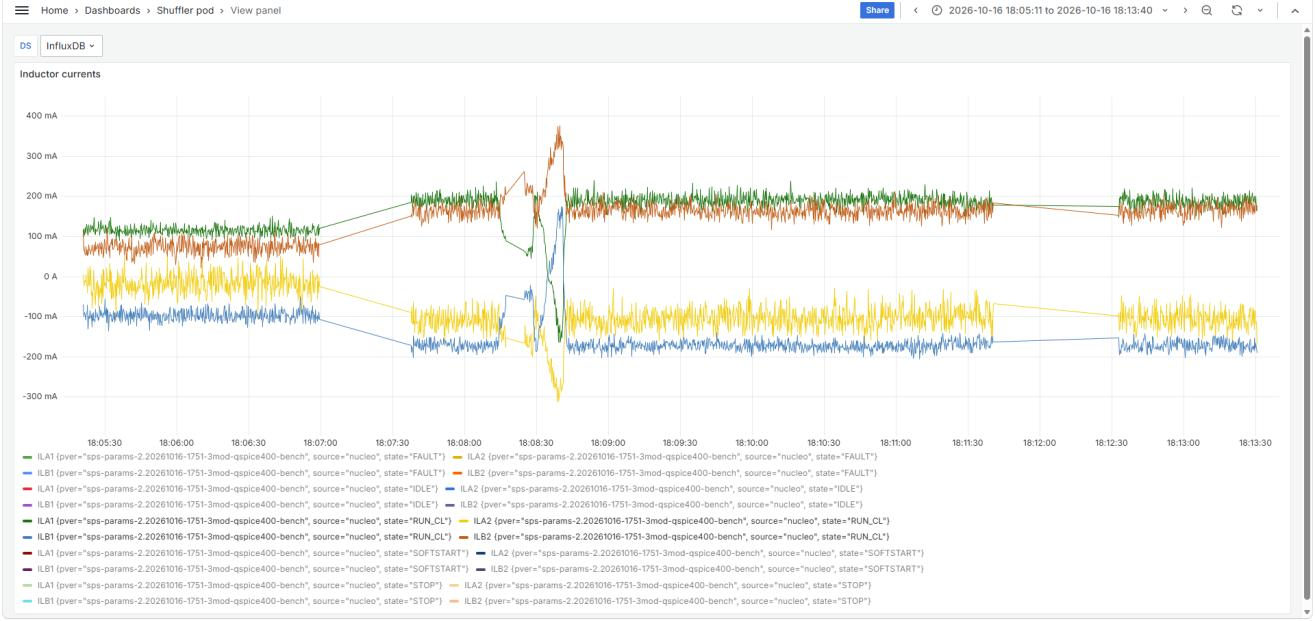
\includegraphics[width=\linewidth]{img-051-119}\caption{Topology and sign conventions.}\end{subfigure}\hfill
  \begin{subfigure}[t]{0.52\linewidth}\centering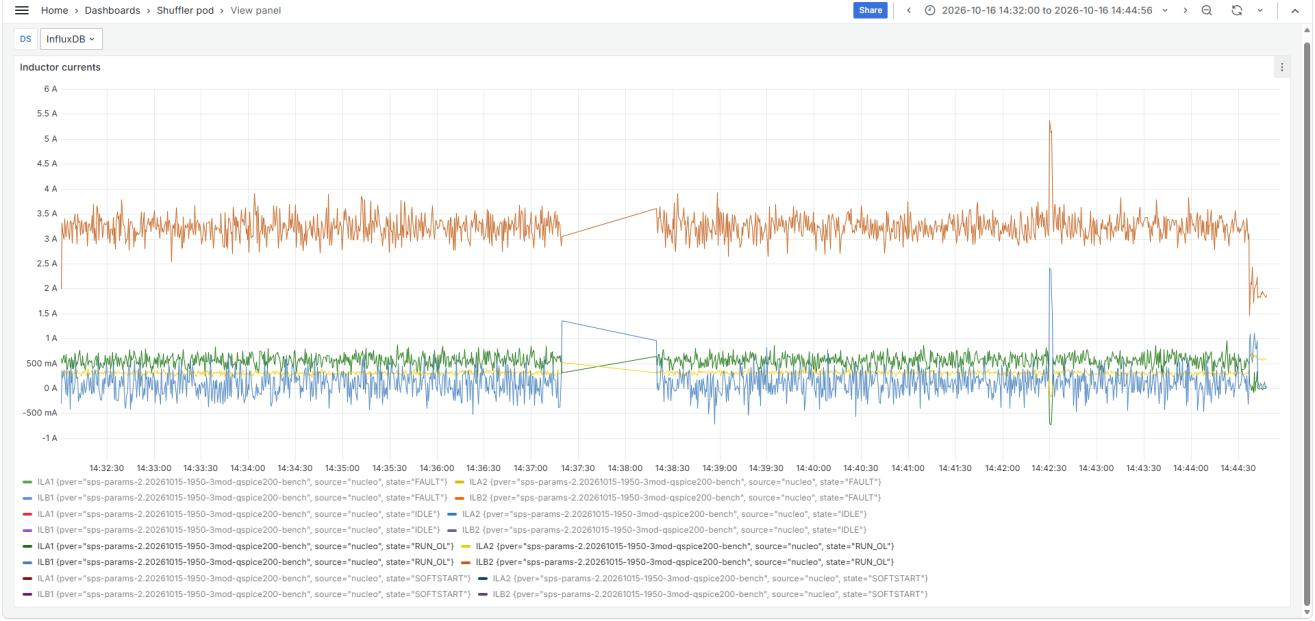
\includegraphics[width=\linewidth]{img-052-123}\caption[{Coupled inductor model}]{Coupled inductor model: $L_k = 0.5L_3$, $L_m = L_2 - 0.5L_3$; ERUC23-4R1K: $R_{DC}$ 1.85\,m$\Omega$, $L_k$ 2.05\,$\mu$H, $L_m$ 5.85\,$\mu$H \cite{tdk_eruc23_ds}.}\end{subfigure}
  \caption{Single-shuffler model elements.}
  \label{fig:single}
\end{figure}

\textbf{State, inputs.} $x = [I_{L1}, I_{L2}, V_{C1}, V_{C2}]^T$, $u_d = [d_A, d_B]^T$, $u_e = [I_{PV1}, I_{PV2}, I_{LOAD}]^T$. $I_{Lk}>0$ flows $V_{mid}\rightarrow L_k\rightarrow$ switch node; $V_{C1} = V_{top}-V_{mid}$, $V_{C2} = V_{mid}$.

\textbf{Switching states.} $2^4=16$ combinations, 7 forbidden (shoot-through), 9 valid; the 4 dual-switch states form the averaged basis with dwell fractions $d_Ad_B$, $d_A(1-d_B)$, $(1-d_A)d_B$, $(1-d_A)(1-d_B)$; the single-switch and all-off states are dead-time transients.

\textbf{Averaged model} (with $\mathbf L = \begin{bmatrix}L & M\\ M & L\end{bmatrix}$):
\begin{align}
  \mathbf L\,\dot{\mathbf I} &= \begin{bmatrix}-d_A V_{C1} + (1-d_A)V_{C2}\\ -d_B V_{C1} + (1-d_B)V_{C2}\end{bmatrix} - R\,\mathbf I\\
  C_1\dot V_{C1} &= d_A I_{L1} + d_B I_{L2} + I_{PV1} - I_{LOAD}\\
  C_2\dot V_{C2} &= I_{PV2} - (1-d_A)I_{L1} - (1-d_B)I_{L2}
\end{align}
Rule: $C_1$ receives current from each phase whose high-side switch conducts; $C_2$ supplies current to each phase whose low-side switch conducts.

\textbf{Equilibrium.} Volt-second balance forces $D_A = D_B \equiv D$ and
\begin{equation}
  \frac{\bar V_{C2}}{\bar V_{C1}} = \frac{D}{1-D},\qquad D = \frac{I_{LOAD}-I_{PV1}}{I_{LOAD}-I_{PV1}+I_{PV2}},\qquad \bar I = \frac{I_{PV2}}{2(1-D)}.
\end{equation}
The differential duty $d_A - d_B$ is a transient input only; a finite load is required for a non-trivial equilibrium.

\textbf{Linearisation and modes.} $\tilde A$ has identical rows 1,2 and columns 1,2 ($L_1 = L_2$). Common-mode duty $\tilde u_c = (\tilde d_A+\tilde d_B)/2$ drives $(I_\Sigma = I_{L1}+I_{L2}, V_{C1}, V_{C2})$; differential duty $\tilde u_\delta = \tilde d_A - \tilde d_B$ drives $I_\Delta = I_{L1}-I_{L2}$ through a pure integrator $L\,\dot{\tilde I}_\Delta = -V_\Sigma \tilde u_\delta$.

\textbf{Stability.} $\sigma(\tilde A) = \{0, 0, \pm j\omega_0\}$, $\omega_0^2 = 2D^2/(LC_1) + 2(1-D)^2/(LC_2)$; with $L = 8.2\uH$, $C = 100\uF$, $D=0.5$: $\omega_0 \approx 34.9$\,krad/s (5.56\kHz), $Z_0 = 0.286\ohm$. With the coupled inductor and $R_w = 1.85$\,m$\Omega$: $-67.3 \pm j26\,968$, $-902$, $0$ ($f_0$ 4.29\,kHz, $\zeta = 0.0025$). The open-loop plant is marginally stable; the controller must provide all damping.

\textbf{Controllability / observability.} Controllable if $\bar I \ne 0$ (no DCM), $V_\Sigma \ne 0$ and $D \in (0,1)$. Observability: $\{V_{C1},V_{C2}\}$ gives rank 3 of 4 (differential current hidden); adding $I_{L1}$ gives rank 4. Per-phase current sensing is therefore mandatory (sensor set of \cref{sec:components}).

\textbf{Discretisation.} ZOH at $T_s = 5\us$: poles $0.9848 \pm 0.1737j$, $1$, $1$ on the unit circle.

\textbf{Cascaded PI (Semester 1 design, superseded).} Crossovers 10\,kHz / 1\,kHz / 5\,kHz, PM 84$^\circ$: $K_{p,i} = 0.00678$, $K_{i,i} = 42.6$; $K_{p,v} = 0.628$, $K_{i,v} = 395$; $K_{p,\delta} = 0.00339$. Three SISO loops treated the coupled states as independent; the fixed-current-reference inner loop drove the shaded module to open circuit (progress report Fig.~8). \Cref{fig:single_portraits} shows the pole map and phase portraits that motivated the MIMO reformulation.

\begin{figure}[htbp]
  \centering
  \begin{subfigure}[t]{0.49\linewidth}\centering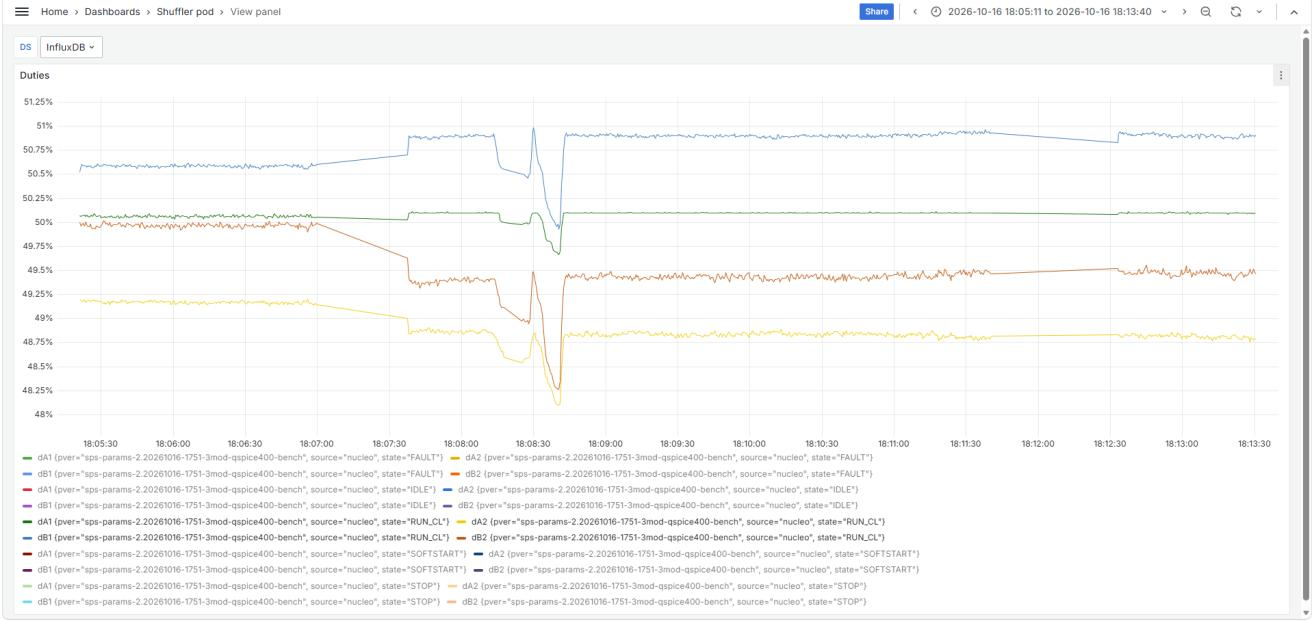
\includegraphics[width=\linewidth]{img-051-121}\caption[{Open-loop eigenvalues}]{Open-loop eigenvalues: idealised model on the $j\omega$ axis; winding resistance and coupling pull the resonant pair into the LHP.}\end{subfigure}\hfill
  \begin{subfigure}[t]{0.49\linewidth}\centering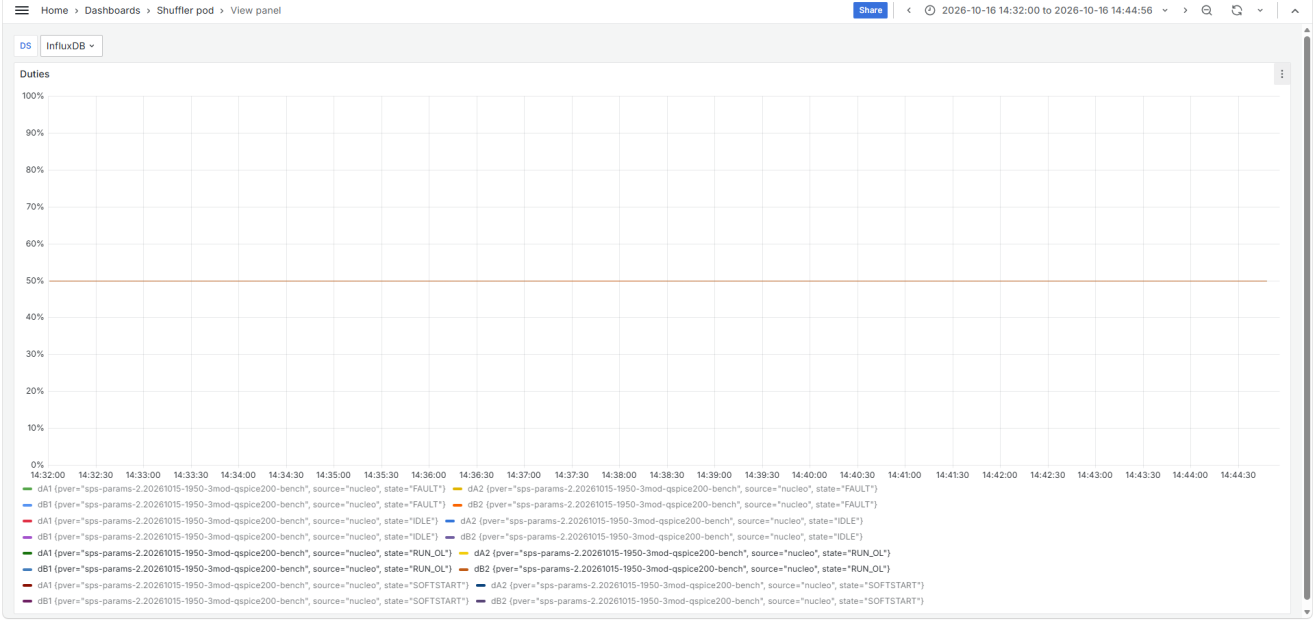
\includegraphics[width=\linewidth]{img-052-125}\caption[{Full 4-state MIMO plant}]{Full 4-state MIMO plant: LQR + integral pulls the resonant pair off the $j\omega$ axis into a well-damped region.}\end{subfigure}\\[3pt]
  \begin{subfigure}[t]{0.75\linewidth}\centering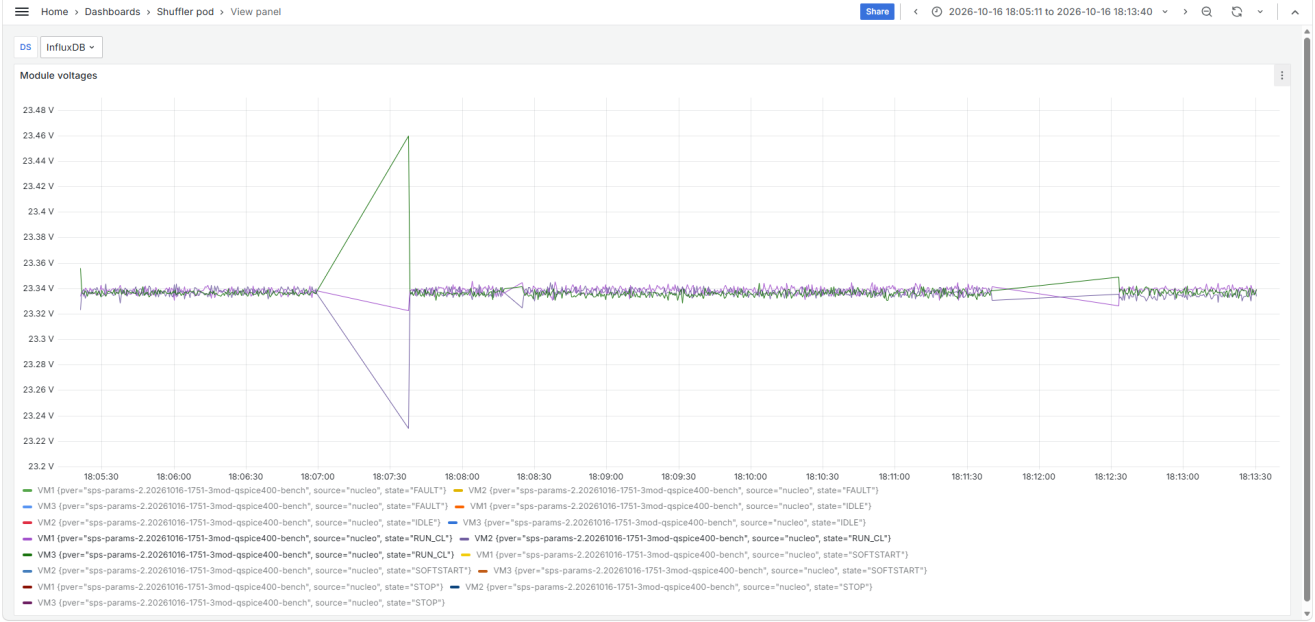
\includegraphics[width=\linewidth]{img-051-120}\caption[{Phase portraits}]{Phase portraits: (a) ideal, centre; (b) passive damping, $\zeta\approx0.003$; (c) inner current loop active, stable focus.}\end{subfigure}
  \caption{Single-shuffler stability pictures (Semester 1 and break).}
  \label{fig:single_portraits}
\end{figure}

\textbf{Re-interpretation after the hardware convention was fixed.} The sensed $I_{LA}+I_{LB}$ \emph{is} the circulating current; relabelled, the Appendix-B model gives $-77$\,V per unit against $-76.5$ measured and $-200$\,A per unit with the 0.386\,$\Omega$ battery-path resistance, so the Semester 1 derivation was right in kind (DESIGN\_LOG 6.1).

\subsection{$N$-module string model (deployed)}
\label{app:nstring}
\begin{figure}[htbp]
  \centering
  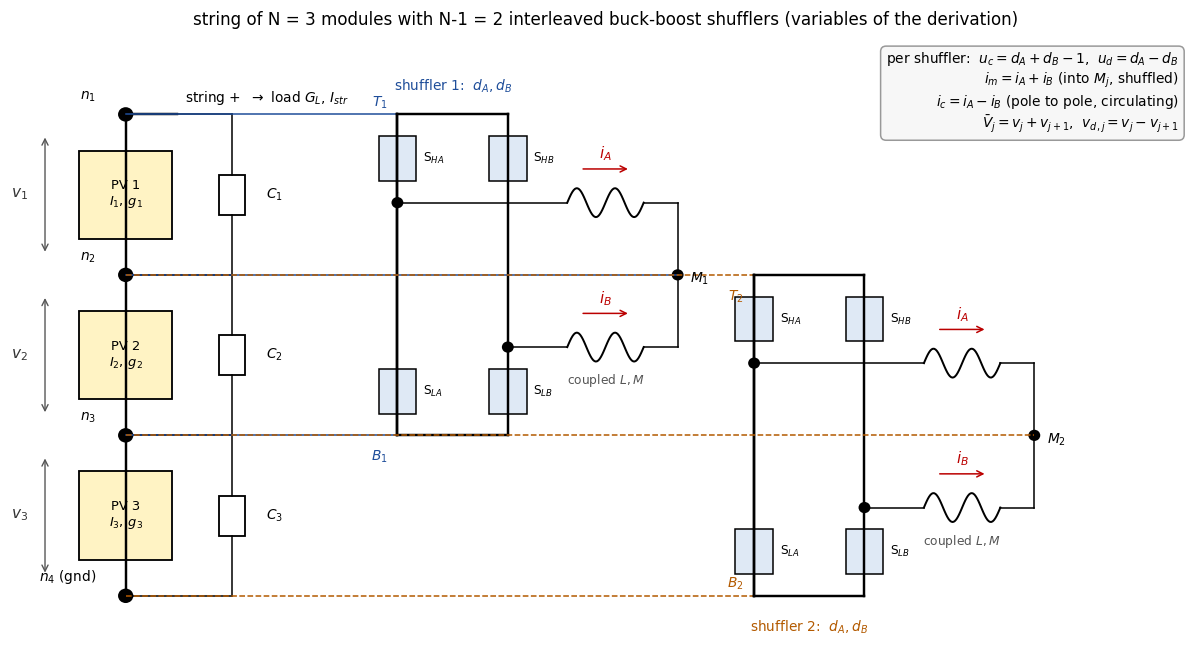
\includegraphics[width=\linewidth]{img-007-011}
  \caption[{Derivation drawing of the $N=3$ string}]{Derivation drawing: $N=3$ modules and $N-1=2$ interleaved buck-boost shufflers with the node potentials and per-shuffler variables of the $N$-module model (the small-signal version is \cref{fig:nodal}).}
  \label{fig:nstring}
\end{figure}
\textbf{Variables} (\cref{fig:nstring}). Node potentials $\phi_k$, $k = 1..N+1$ (node $N+1$ is ground); module voltage $v_k = \phi_k - \phi_{k+1}$. Shuffler $j$ spans modules $j$, $j+1$: rails $\phi_j$, $\phi_{j+2}$, midpoint $\phi_{j+1}$, $\Vbar_j = v_j + v_{j+1}$. Modal duties $\uc = d_A + d_B - 1$, $\ud = d_A - d_B$ (inverse $d_A = \tfrac12(1+\uc+\ud)$, $d_B = \tfrac12(1+\uc-\ud)$). Modal currents $\im = i_A + i_B$ (shuffled; telemetry $I_{LA} - I_{LB}$ because the B sensor is reversed) and $\ic = i_A - i_B$ (circulating; telemetry $I_{LA}+I_{LB}$). Outputs $\vd{}_{,j} = v_j - v_{j+1} = \phi_j - 2\phi_{j+1} + \phi_{j+2}$ and $\ic{}_{,j}$.

\textbf{State equations} (\cref{eq:wind1,eq:wind2,eq:nodal}): $S$ injects $+1$ at the midpoint and $-\tfrac12$ at each rail of shuffler $j$; $G_n$ is the nodal conductance of the module slopes $g_k$ with $G_{load}$ added at node 1; $w$ the module short-circuit current injections. Rail currents are $\tfrac12\im(1\pm\uc) \pm \tfrac12\ic\ud$.

\textbf{Inductances.} As built (ERUC23 windings 1:$-$1) the circulating mode sees $L+M = 13.75\uH$ and the shuffled mode $L-M = 2.05\uH$ ($L_{self} = 7.9\uH$, $M = 5.85\uH$). The ripple law $\Delta\ic = \Vbar/(2\fsw(L+M))$ confirms the assignment (\cref{tab:T6}).

\textbf{Equilibrium.} $D_j\Vbar_j = v_{j+1} + \tfrac12 R_m I_{m,j}$ $\Rightarrow$ $D_j/(1-D_j) = v_{j+1}/v_j$. Charge balance on the ladder: $T(N)\,I_m = \delta I$, $T = \mathrm{tridiag}(-\tfrac12, 1, -\tfrac12)$, $(\delta I)_j = I_j - I_{j+1}$, with the closed form $T^{-1}_{jk} = \tfrac{2}{N}\min(j,k)(N-\max(j,k))$; string current $I_{str} = I_1 - D_1 I_{m,1} = \tfrac1N\sum_k I_k$. For $N=3$: $i_{m1} = (4I_1 - 2I_2 - 2I_3)/3$. Open loop at $D = 0.5$: $\vd{}_{,j} = -R_m \im{}_{,j}$. Check against QSPICE S10i ($R_m = 0.29\ohm$): $\im = -0.466/-0.534\A$ (model) vs $-0.464/-0.539\A$ (QSPICE); $I_{str}$ 1.032 vs 1.024\,A; $R_m\im = -0.135\V$ vs $\vd{}_{,1} = -0.135\V$.

\textbf{DC gain.}
\begin{equation}
  G(N) = \begin{bmatrix} G_v & 0\\ 0 & \mathrm{diag}(\Vbar_j/R_c)\end{bmatrix},\qquad
  G_v = -(R_m I + Z_e)^{-1} Z_e\,\mathrm{diag}(\Vbar_j),\qquad Z_e = -D_v G_n^{-1} S,
\end{equation}
where $D_v$ maps $\phi \mapsto \vd$. $G(2)$: $-\Vbar/(R_m g + 1)$. $G(3)$ voltage block: diagonal $-\Vbar(4R_m g + 3)/(4R_m^2g^2 + 8R_m g + 3)$, off-diagonal $2R_m\Vbar{} g/(\cdot)$: diagonal $\approx -\Vbar$ with $O(R_m g)$ neighbour terms. Numbers in \cref{tab:G}.

\textbf{Controller.} $M = G^{-1}\mathrm{diag}(k_I)$ with $k_{I,v} = 2\pi\cdot150$\,s$^{-1}$, $k_{I,i} = 2\pi\cdot400$\,s$^{-1}$; $u = k\,(M_p e + M\xi)$, $M_p = M\,\mathrm{diag}(k_{p,v},k_{p,v},k_{p,i},k_{p,i})$, $k_{p,v} = 1.58\times10^{-4}$\,s, $k_{p,i} = 1.08\times10^{-4}$\,s, $\xi \mathrel{+}= T_s e$, $T_s = 100\us$, first-order LPF on $y$ with $f_c = 2\kHz$ ($a = 2\pi f_c T_s/(1+2\pi f_c T_s) = 0.557$), one tick of delay; back-calculation anti-windup $\xi = M^{-1}(u_{act} - M_p e)$. Firmware layout $u = [\uc{}_{,1},\uc{}_{,2},\ud{}_{,1},\ud{}_{,2}]$, $e = [e_{vd1}, e_{vd2}, e_{ic1}, e_{ic2}]$. Design: $\tau_v = 1/(k\,k_{I,v})$, $\tau_i = 1/(k\,k_{I,i})$, rise $= 2.197\tau$, 2\,\% settle $= 3.91\tau$.

\begin{table}[htbp]\centering\small
\caption{Design time constants vs gain scale and the closed-loop pole frequencies at $k=1$.}
\label{tab:design_tau}
\begin{tabular}{l r r r l}
\toprule
$k$ & $\tau_v$ [ms] & $\tau_i$ [ms] & rise $2.197\tau_v$ [ms] & closed-loop poles at $k=1$\\
\midrule
0.1 & 10.61 & 3.98 & 23.3 & model $M$: 160 / 164\,Hz ($\vd$), 593\,Hz ($\ic$)\\
0.3 & 3.54 & 1.33 & 7.8 & deployed $M$: 127 / 135\,Hz ($\vd$), 582 / 604\,Hz ($\ic$)\\
1.0 & 1.06 & 0.40 & 2.3 & \\
\bottomrule
\end{tabular}
\end{table}

\textbf{Plants used in the analysis.} PV80 ($N=3$): $V = 20.5\V$, $g = 0.19$\,S per module, $C = [130, 260, 130]\uF$, $G_{load} = 20$\,S (DL3021 CV), $R_w = 0.061\ohm$ (averaged) or $R_{sw}$. BENCH-QSPICE: $V = 23.3\V$, $g = 0$, $I = [0.8, 1.0, 1.3]\A$ (all NGE103 channels in current limit, the 16 Oct point), same $C$. Reduced voltage mode: $f_0 = 1/(2\pi\sqrt{L_m C_e})$ with $C_e = 173\uF$ gives 8.4\,kHz; $\zeta = \tfrac12(R_m\sqrt{C_e/L_m} + g_e\sqrt{L_m/C_e})$ = 0.29 at 61\,m$\Omega$, 1.34 at 0.29\,$\Omega$, 7.8 at 1.7\,$\Omega$.

\textbf{PBH ranks (PV80).} $n = 7$ states; controllable from $u$ (7), from $\uc$ alone (5), from $\ud$ alone (2); observable from $y$ (7), from $\vd$ alone (5): circulating modes are reachable only from $\ud$ and seen only by the current sensors; the string-sum mode (176\,Hz with a current sink) is unreachable/unobservable with equal capacitors and belongs to the load / MPPT. cond$(G(N))$ for PV80 grows only from 16.6 ($N=2$) to 18.9 ($N=8$), i.e.\ the decoupling scales.

\begin{figure}[htbp]
  \centering
  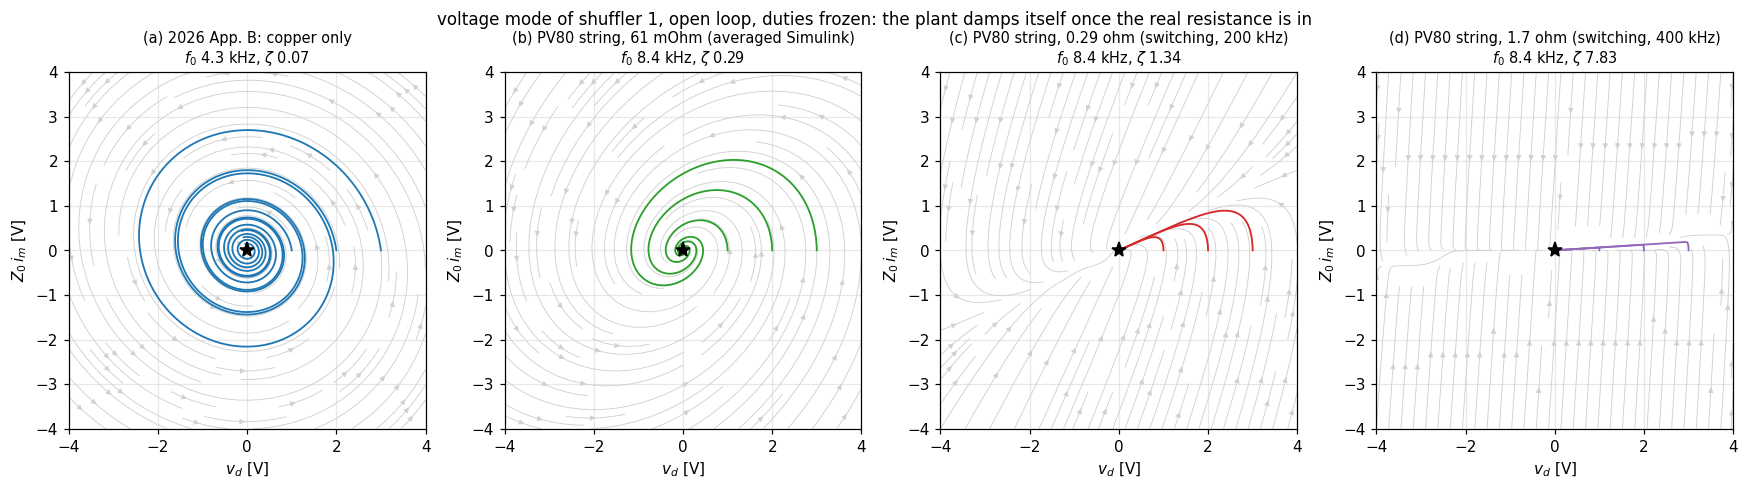
\includegraphics[width=\linewidth]{img-011-012}
  \caption[{Open-loop phase portraits of the voltage mode in the $(\vd,\,Z_0\im)$ plane}]{Open-loop phase portraits of the voltage mode in the $(\vd,\,Z_0\im)$ plane: (a) 2026 App.~B copper-only model ($\zeta\approx0.07$), (b) PV80 plant with the 61\,m$\Omega$ averaged resistance (focus, $\zeta\approx0.3$, 7--9\,kHz), (c) 0.29\,$\Omega$ switching plant at 200\,kHz and (d) 1.7\,$\Omega$ at 400\,kHz (over-damped nodes). The plant damps itself once the real switching resistance is included.}
  \label{fig:ana_portraits}
\end{figure}

\begin{figure}[htbp]
  \centering
  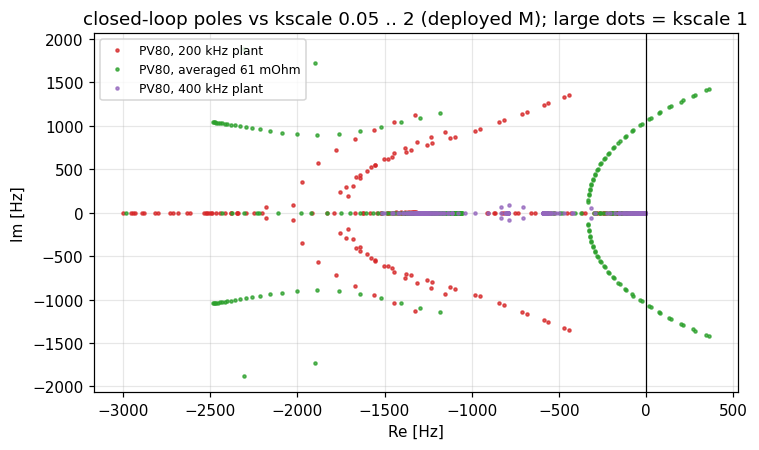
\includegraphics[width=0.68\linewidth]{img-012-014}
  \caption[{Closed-loop poles of the analytical $N=3$ model as the gain scale $k$ is swept}]{Closed-loop poles of the analytical $N=3$ model with the deployed gain set as $k$ is swept from 0.05 to 2, for the 200\,kHz (0.29\,$\Omega$), averaged (61\,m$\Omega$) and 400\,kHz (1.7\,$\Omega$) plants; large dots mark $k=1$.}
  \label{fig:ana_rl}
\end{figure}

\subsection{Switching resistance $R_{sw}$}
\label{app:rsw}
The averaged 61\,m$\Omega$ plant over-predicts the current-loop gain $5\times$. Open-loop $\ud$ sweeps on the QSPICE device model (S10i / S10i3 / S10i4) with and without reverse recovery and device capacitances isolate the mechanism: pole-capacitance commutation during the dead time costs volt-seconds proportional to the current,
\begin{equation}
  R_{sw} = \frac{4\Vbar^2 C_p \fsw}{\Delta i^2} = 64\,C_p\,\fsw^3\,(L+M)^2,
\end{equation}
which with $C_p = 2.2$\,nF gives 0.21 / 0.72 / 1.70\,$\Omega$ at 200 / 300 / 400\,kHz; the identified gains (142 / 58 / 23\,A per unit) imply 0.27 / 0.79 / 1.66\,$\Omega$; the analysis uses 0.29 / 0.80 / 1.70\,$\Omega$. The switching twin (\code{nswitch.py}, exact per-configuration integration with $C_p = 2C_{oss}$) reproduces QSPICE point for point (170/165/148/111/74/66 vs 172/163/148/112/71/66\,A per unit).

\subsection{Open items}
Unexplained 6.34\,kHz / $\zeta$ 0.53 resonance seen in June 2026; $C_{oss}$ is voltage dependent so $R_{sw}$ should be re-measured per operating point; the $\ud\rightarrow\vd$ cross term ($-10\ldots-25$\,V per unit) is not in the model; at 400\,kHz the dead time sits at the ZVS boundary and the linear model stops near $\ud\approx0.02$.

\section{Controller, Supervisor and Firmware Pseudocode}
\label{app:pseudo}
% Based on 6_RTOS/ctrl_core/*.c and 6_RTOS/App/app.c (the same C runs in SIL, the
% QSPICE DLL and the firmware).  Simplified; see the sources for the exact code.

\begin{lstlisting}[caption={MIMO decoupling PI, one 100\,$\mu$s tick (\code{shuffler\_ctrl.c}).},label={lst:ctrl}]
function ctrl_step(VM[1..N], IL_A[1..NS], IL_B[1..NS], rv[1..NS], Vref[1..NS]):
    # outputs: module-voltage differences and circulating currents
    y = [VM[1]-VM[2], ..., VM[N-1]-VM[N],  IL_A[1]+IL_B[1], ..., IL_A[NS]+IL_B[NS]]
    y_f += a * (y - y_f)                       # LPF, a = 2*pi*fc*Ts/(1+2*pi*fc*Ts), fc = 2 kHz
    r   = [rv + Vref, 0 ... 0]  # supervisor relaxation + manual offsets; ic refs are zero
    e   = r - y_f
    xi_try = xi + Ts * e                       # integrator candidate
    u   = kscale * (Mp @ e + M @ xi_try)       # u = [uc1..ucNS, ud1..udNS]; M = inv(G) diag(kI)
    for each shuffler j:
        dA[j] = clamp(0.5 + 0.5*(u[j] + u[NS+j]), dmin, dmax)
        dB[j] = clamp(0.5 + 0.5*(u[j] - u[NS+j]), dmin, dmax)
    u_act = [dA + dB - 1, dA - dB]             # what was actually applied
    xi = Minv @ (u_act / kscale - Mp @ e)      # back-calculation anti-windup (every tick)
    return dA, dB
\end{lstlisting}

\begin{lstlisting}[caption={Feasibility governor / supervisor, 1\,ms (\code{shuffler\_supervisor.c}).},label={lst:sup}]
function supervisor_step(IM[1..N], IL_A, IL_B, d[1..NL], en):
    if not en: beta = 0; rv = 0; return rv
    id   = IL_A - IL_B                          # shuffled current per shuffler
    imf += alpha * (IM - imf);  idf += alpha * (id - idf)      # alpha = Ts3/TF = 0.2
    dl   = max(imf) - imf                       # deficit of each module vs the strongest
    stress = max( max|idf| / I_RATED,  max|d - 0.5| / 0.45 )  # I_RATED = 10 A
    if   stress > S_HI: beta += Ts3 * KB   * (stress - S_HI)   # S_HI 0.9, KB 60
    elif stress < S_LO: beta -= Ts3 * KREL * (S_LO - stress)   # S_LO 0.7, KREL 6
    beta = clamp(beta, 0, BMAX)                                 # BMAX 4
    for each shuffler k: rv[k] = clamp(beta * (dl[k+1] - dl[k]), -RVMAX, RVMAX)   # 30 V
    return rv                                   # relaxes equalisation when a shuffler is stressed
\end{lstlisting}

\begin{lstlisting}[caption={Module-current reconstruction by KCL (\code{shuffler\_recon.c}); the string current is unobservable so $I_N = 0$ is the reference.},label={lst:recon}]
function recon(IL_A, IL_B, dA, dB):
    for each shuffler k:
        ia = IL_A[k]; ib = -IL_B[k]            # B sensor is reversed on the board
        itop[k] = dA[k]*ia + dB[k]*ib          # averaged current drawn at the top rail
        ic[k]   = ia + ib                      # injected at the midpoint
        ibot[k] = ic[k] - itop[k]              # returned at the bottom rail
    IM[N] = 0
    for j = N-1 down to 1:
        IM[j] = IM[j+1] + ic[j] - (j < NS ? itop[j+1] : 0) - (j >= 2 ? ibot[j-1] : 0)
    return IM                                   # relative module currents (offset-free deficits)
\end{lstlisting}

\begin{lstlisting}[caption={Adaptive-step perturb-and-observe MPPT, 1\,ms (\code{shuffler\_mppt.c}); compiled in but disabled on hardware because the load performs the string MPPT.},label={lst:mppt}]
function mppt_step(Vstr, Istr, beta, en):
    if not en: Iref = IREF0; dir = +1; boot = 1; return Iref      # IREF0 8 A
    acc += Vstr * Istr; n += 1
    if n == NWIN:                                                  # 20 ticks = 20 ms
        P = acc / NWIN; acc = 0; n = 0
        if |beta - beta0| > 1e-3: boot = 1          # governor moved: hold the reference
        elif boot: Pprev = P; Iref += dir * S0; boot = 0           # S0 0.25 A
        else:
            dP = P - Pprev
            step = clamp(KA * |dP|, SMIN, SMAX)                    # 0.01, 0.05 .. 1 A
            if   dP >  DB: Iref += dir * step                      # DB 1 W
            elif dP < -DB: dir = -dir; Iref += dir * step
            Pprev = P
        beta0 = beta; Iref = clamp(Iref, IMIN, IMAX)               # 2 .. 8.5 A
    return Iref
\end{lstlisting}

\begin{lstlisting}[caption={Control ISR, 10\,kHz (HRTIM master repetition interrupt, \code{app.c}).},label={lst:isr}]
on HRTIM_master_repetition:                     # every 20 / 30 / 40 PWM periods
    Sensors_Tick()  # 80-sample means per channel; OC / rail / DMA-stall latch
    IL = Sensors_Current_A()                    # (code - zero) * 3300/4096 mV / (100 mV/A)
    if Sensors_FaultLatched(): trip(FLT_OC_LATCH)
    prt_isr_service()  # pending C,APPLY: swap gains, xi = Minv * u_act(d)
    VM = snapshot of the 1 kHz INA task (VM1 from vstr_pi - VM2 - VM3 when vm1_src = 2)
    if state == SOFTSTART:
        d = ramp(d_start, target, n_tick / 1500)          # 150 ms linear ramp
    elif state == RUN and mode is CL:
        out = stack_step({VM, IL, Vstr = sum VM, Vref, en_sup, en_mppt = 0})
        d = clamp(out.d, d_prev - slew, d_prev + slew)    # slew 0.01 per tick
    elif state == RUN:  d = open-loop duties (C,DUTY / C,DUTYS)
    else:               d[i] = Vbot / (Vtop + Vbot)       # pre-bias while idle (0.5 if unknown)
    for each leg: hw_set_duty(leg, d)          # clamp to the f_sw limits, write CMP1 (preloaded)
\end{lstlisting}

\begin{lstlisting}[caption={Stack scheduler (\code{stack.c}): controller every tick, supervisory layers every 10th.},label={lst:stack}]
function stack_step(in):
    if tick % STACK_DECIM == 0:                 # 10 -> 1 kHz
        IM   = recon(in.IL_A, in.IL_B, dA, dB)
        rv   = supervisor_step(IM, in.IL_A, in.IL_B, d, in.en_sup)
        Iref = mppt_step(in.Vstr, in.Istr, beta, in.en_mppt)
    dA, dB = ctrl_step(in.VM, in.IL_A, in.IL_B, rv_delayed, in.Vref)   # rv through a unit delay
    tick += 1
    return {dA, dB, rv, beta, stress, IM, Iref}
\end{lstlisting}

\begin{lstlisting}[caption={Safety task and state machine, 100\,Hz (\code{app.c}); \code{trip()} may run from any context.},label={lst:fsm}]
every 10 ms:
    kick IWDG                                    # 0.3 s window
    if state in {RUN, SOFTSTART}:
        if E-stop pin low:                      trip(FLT_ESTOP)
        OV / UV / string-OV counters: 3 consecutive samples -> trip(code)   # 30 V, 3 V (CL), 85 V
        if CL and now - last_rx > wdg_s:        trip(FLT_COMMS_WDG)         # 5 s without a C line
        if CL and vm1_src == 2 and VM1 stale:   trip(FLT_VSTR_STALE)
        if any INA die > 85 C:                  trip(FLT_OVERTEMP)
        if CL and a needed VM unreadable:       trip(FLT_INA)
    switch state:
        IDLE:      if enable and mode != IDLE: pins -> HRTIM; arm synchronised enable; state = SOFTSTART
        SOFTSTART: if not enable: state = STOP;  elif ramp done: stack_init(); state = RUN
        RUN:       if not enable or mode == IDLE: state = STOP
        STOP:      legs off; enable = 0; state = IDLE
        FAULT:     hw_outputs_off()             # every 10 ms until C,CLEAR
    send S line on every state change; send F line once per latched fault

function trip(code):
    hw_outputs_off(); gates low                 # first, from any context
    faults |= code; enable = 0; state = FAULT
\end{lstlisting}

\begin{lstlisting}[caption={Soft start (\code{app.c} + \code{hw\_legs\_enable\_sync}).},label={lst:softstart}]
while IDLE: every leg pair is held at d0 = Vbot / (Vtop + Vbot)    # matches the natural midpoint
on enable: outputs switch on at master CMP1 = PER/4 (centred first pulse, 16-try fallback window)
SS_TICKS = 150 ms * 10 kHz = 1500
tick 0: d_start[i] = d_applied[i]
each tick n: frac = min(n / SS_TICKS, 1)
    target = 0.5 if CL else OL duty[i]
    d[i] = d_start[i] + (target - d_start[i]) * frac
n == SS_TICKS: ss_done -> safety task moves to RUN; stack_init() so the controller starts from zero integrators
\end{lstlisting}

\begin{lstlisting}[caption={Pi pod main loops (\code{pod.py}, \code{eload.py}).},label={lst:pod}]
pod.py:
    RX thread: read line from /dev/ttyACM0 @ 921600 -> telemetry_parser.parse_line(line)
               -> InfluxDB points (telemetry / status / fault / note / cmd), batched 200 pts / 500 ms
    TX thread: one byte every 2 ms (firmware RX is one IRQ per byte); C,PING every 1 s (comms watchdog)
    main loop (0.2 s): DS18B20 heatsink temperature -> Influx (C,ESTOP if > 80 C); LCD state/values; RGB LED by state
    control socket 127.0.0.1:5017: podctl / params_web / remote.py send commands; IR keys -> presets (actions.py)
eload.py:
    5 Hz:  :MEAS:VOLT? :MEAS:CURR? :MEAS:POW?  -> Influx (source = eload)
    1 Hz:  mode, levels, ranges, questionable status
    2 Hz:  C,SET,vstr_pi,<V>  -> Nucleo (VM1 source when U10 is unreadable)
\end{lstlisting}

\section{Firmware, Peripherals and Telemetry Contract}
\label{app:firmware}

\subsection{Scheduling}
\begin{table}[htbp]\centering\small
\caption{Execution contexts of the firmware (bare-metal superloop plus interrupts; no RTOS).}
\label{tab:sched}
\begin{tabularx}{\linewidth}{p{3.5cm} p{3.2cm} p{1.6cm} X}
\toprule
Context & Trigger / priority & Rate & Work\\
\midrule
\code{app\_ctrl\_isr} & HRTIM master repetition IRQ, NVIC prio 1 & 10\,kHz ($T_s = 100\us$) & hall averages + OC latch, gain swap, soft-start / \code{stack\_step} / OL duties / pre-bias, slew limit, write CMP1\\
\code{app\_tick\_1ms} & SysTick, prio 0 & 1\,kHz & ms counter; main-loop stall check ($>20\ms$ while switching $\Rightarrow$ fault 0x2000)\\
\code{app\_task\_sense\_v} & main loop & 1\,kHz & INA239 $\times$3 over SPI3 $\rightarrow V_{M1..3}$, die temperatures\\
\code{app\_task\_safety} & main loop, every 10th pass & 100\,Hz & IWDG kick, OV/UV/string-OV, watchdogs, state machine\\
\code{app\_task\_telemetry} & every 20th pass & 50\,Hz & \code{T} frame; \code{S} line at 1\,Hz and on state change\\
\code{app\_task\_cmd} & every pass & 1\,kHz & parse \code{C,...} lines, answer \code{A,...}\\
E-stop & EXTI0 on PC0, prio 0 & event & \code{trip(FLT\_ESTOP)}\\
LPUART1 RX & prio 6, 1 byte per IRQ & event & 512-byte ring buffer\\
\bottomrule
\end{tabularx}
\end{table}
Clock: HSI 16\,MHz $\rightarrow$ PLL $\rightarrow$ SYSCLK 170\,MHz (AHB/APB 170\,MHz, flash latency 4, boost scale); the 400\,kHz build feeds the ADCs from PLL-P at 56.7\,MHz. IWDG 0.3\,s. ISR cost is measured with the DWT cycle counter against the 100\,$\mu$s budget (Release \code{-O2}; \code{-O0} reached 75\,$\mu$s idle and $>100\,\mu$s in CL at 300\,kHz). Toolchain: CMake $\ge$ 3.22, Ninja, arm-none-eabi-gcc (Cortex-M4F, hard float, nano specs), presets Debug/Release; \code{build\_wsl.sh} uses the Windows STM32Cube bundle from WSL.

\subsection{Board routing and current sampling}
\begin{figure}[htbp]
  \centering
  \begin{subfigure}[t]{0.42\linewidth}\centering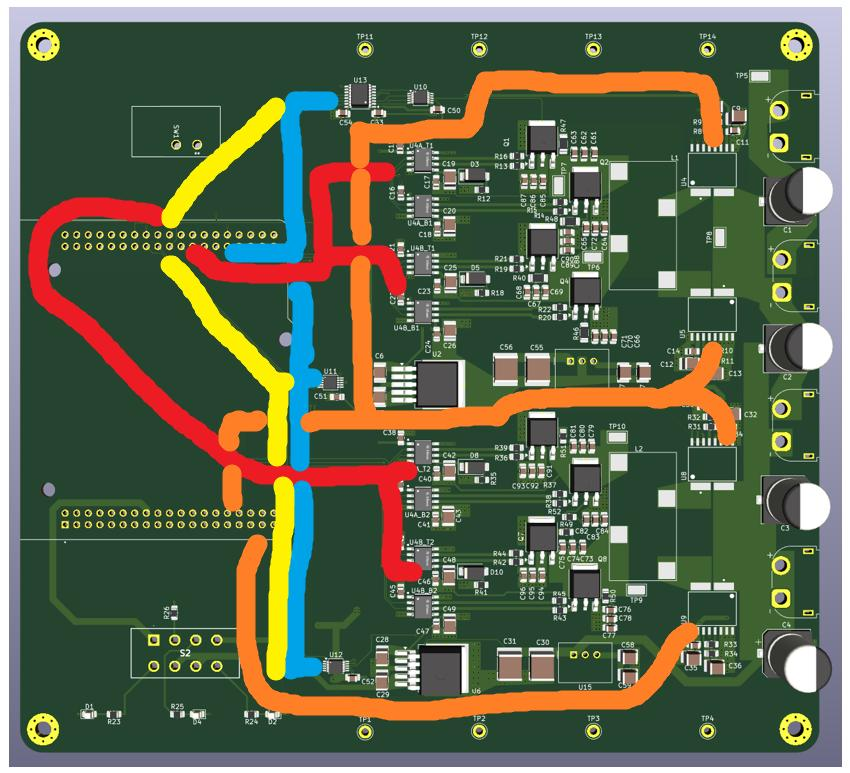
\includegraphics[width=\linewidth]{img-018-026}\caption[{Routing on the Version 0 board}]{Routing on the Version 0 board: PWM (red), SPI (blue), chip selects (yellow), ADC (orange), top and bottom layers.}\end{subfigure}\hfill
  \begin{subfigure}[t]{0.55\linewidth}\centering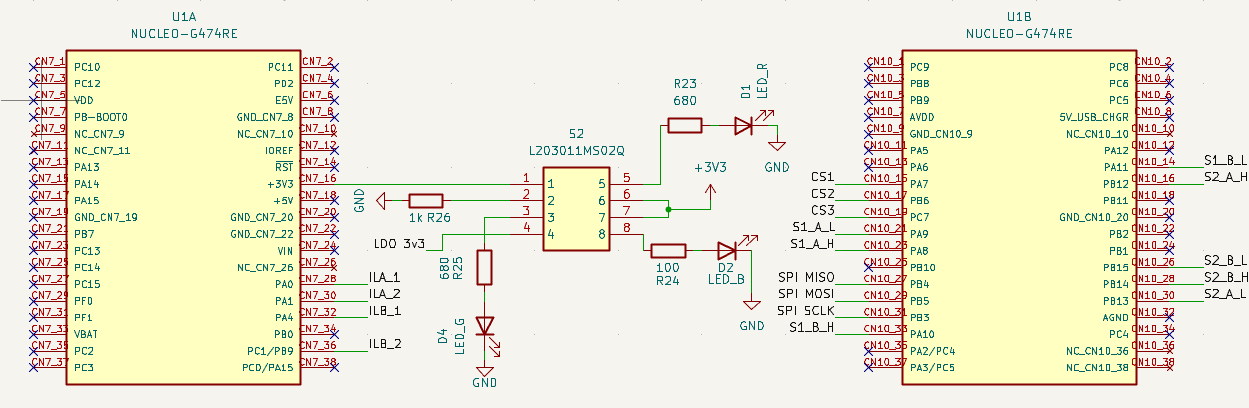
\includegraphics[width=\linewidth]{img-018-028}\caption{Nucleo header pinout used by the PCB.}\end{subfigure}
  \caption{Controller routing on the Version 0 PCB.}
  \label{fig:routing}
\end{figure}
\begin{figure}[htbp]
  \centering
  \resizebox{0.95\linewidth}{!}{% Hall-current sampling: 4 ADC triggers per PWM period from the HRTIM, 80-sample box average per control tick
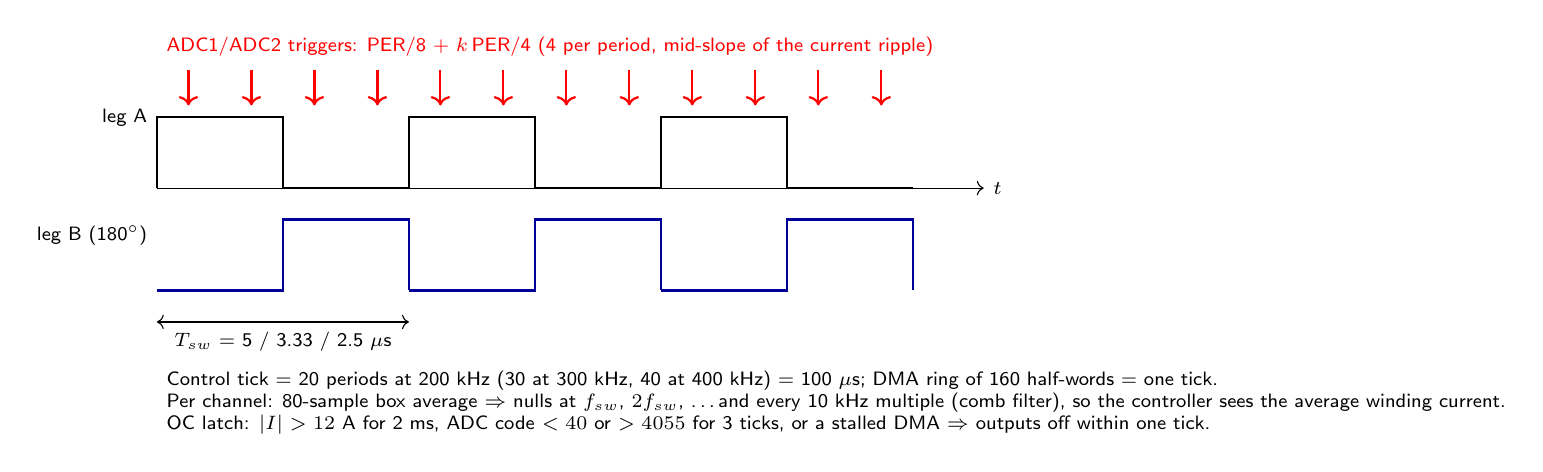
\begin{tikzpicture}[x=1cm,y=1cm,font=\sffamily\scriptsize]
  % PWM period axis
  \draw[->] (0,0) -- (10.5,0) node[right]{$t$};
  \foreach \i in {0,1,2}{
    \draw[thick] (\i*3.2,0) -- (\i*3.2,0.9) -- (\i*3.2+1.6,0.9) -- (\i*3.2+1.6,0) -- (\i*3.2+3.2,0);
  }
  \node[left] at (0,0.9) {leg A};
  \foreach \i in {0,1,2}{
    \draw[thick,blue!60!black] (\i*3.2,-1.3) -- (\i*3.2+1.6,-1.3) -- (\i*3.2+1.6,-0.4) -- (\i*3.2+3.2,-0.4) -- (\i*3.2+3.2,-1.3);
  }
  \node[left] at (0,-0.6) {leg B (180$^\circ$)};
  % triggers at PER/8 + k PER/4
  \foreach \i in {0,1,2}{\foreach \k in {0,1,2,3}{
    \draw[red,thick,->] (\i*3.2+0.4+\k*0.8,1.5) -- (\i*3.2+0.4+\k*0.8,1.05);
  }}
  \node[red,anchor=south west] at (0,1.55) {ADC1/ADC2 triggers: PER/8 + $k$\,PER/4 (4 per period, mid-slope of the current ripple)};
  \draw[<->] (0,-1.7) -- node[below]{$T_{sw}$ = 5 / 3.33 / 2.5 $\mu$s} (3.2,-1.7);
  \node[align=left,anchor=north west] at (0,-2.2) {Control tick = 20 periods at 200 kHz (30 at 300 kHz, 40 at 400 kHz) = 100 $\mu$s; DMA ring of 160 half-words = one tick.\\
  Per channel: 80-sample box average $\Rightarrow$ nulls at $\fsw$, $2\fsw$, \ldots and every 10 kHz multiple (comb filter), so the controller sees the average winding current.\\
  OC latch: $|I| > 12$ A for 2 ms, ADC code $<40$ or $>4055$ for 3 ticks, or a stalled DMA $\Rightarrow$ outputs off within one tick.};
\end{tikzpicture}
}
  \caption[{Hall-current sampling scheme}]{Hall-current sampling scheme: four HRTIM-triggered ADC conversions per switching period, box-averaged over one control tick.}
  \label{fig:adc}
\end{figure}

\subsection{Peripherals}
\begin{table}[htbp]\centering\scriptsize
\caption{Peripheral configuration (\code{shuffler\_hw.c/h}, \code{sensors.c}, \code{ina2x9.c}, \code{comms.c}).}
\label{tab:periph_full}
\begin{tabular}{l p{12.2cm}}
\toprule
HRTIM1 & $f_{HRTIM} = 170\,\mathrm{MHz}\times32 = 5.44$\,GHz (184\,ps). Master PER 27200 (200\,kHz) / 18133 (300) / 13600 (400). Legs A--D: A legs reset on master PER, B legs on master CMP2 = PER/2 (180$^\circ$ interleave). Duty = leg CMP1, preloaded, update on reset. Output 1 set on the master event, reset on CMP1; output 2 is the complement from the dead-time generator. Dead time \code{HW\_DEADTIME\_NS} 100 (136 steps $\times$ 0.735\,ns, both edges; was 200\,ns until 16 Oct). Pins: leg 0 S1A PA8/PA9, leg 1 S1B PA10/PA11, leg 2 S2A PB12/PB13, leg 3 S2B PB14/PB15 (AF13); a constructor drives them low before \code{main()}. Duty limits 0.05--0.95 (200\,kHz), 0.08--0.95 (300), 0.12--0.88 (400). Synchronised enable at master CMP1 = PER/4. Hardware fault inputs not used (COMP/DAC OC trip reserved, bit 0x002).\\
ADC1 / ADC2 & 12-bit, regular group of 2 ranks, trigger HRTIM ADC trigger 1 = TA CMP3/CMP4 + TB CMP3/CMP4 (4 per period at PER/8 + $k$PER/4). Sample time 6.5 cycles, clock PCLK/4 = 42.5\,MHz, no oversampling, offset calibration at start. ADC1 IN1 = PA0 ($I_{LA1}$), IN2 = PA1 ($I_{LA2}$); ADC2 IN17 = PA4 ($I_{LB1}$), IN7 = PC1 ($I_{LB2}$). DMA1 ch1/ch2 circular half-word, 160 samples = 4 triggers $\times$ 20 periods $\times$ 2 ranks = one control tick; the ISR polls the TC flags.\\
Hall conversion & $I = (\overline{\mathrm{code}} - \mathrm{zero})\cdot(3300/4096\,\mathrm{mV})/S$, $S = 100$\,mV/A on all four channels (B phases were 25 before 16 Oct; \code{params.yaml} still carries 25 for channels 1/3); nominal zero 2048 (1.65\,V); boot zero-cal averages 64 ticks, falls back to 2048 and sets \code{FLT\_ZEROCAL} if off by $>\pm124$ codes. B-phase sensors are physically reversed. Run-time \code{hall\_mva0..3} ($\pm$400, $|x|\ge10$), \code{hall\_zero0..3} (1800--2300). Box average of 80 samples per channel per tick (nulls at $\fsw$, $2\fsw$, \ldots and every 10\,kHz multiple). OC latch: $|I| > $ \code{oc\_a} (12\,A) for 20 ticks, code $<40$ or $>4055$ for 3 ticks, or DMA not wrapping for 3 ticks.\\
SPI3 & Master, mode 1, 8-bit MSB-first, software NSS, prescaler 128 $\Rightarrow$ 1.33\,MHz; PB3 SCK, PB4 MISO, PB5 MOSI; CS1 PA7 (U12, PV3+ to GND), CS2 PB6 (U11, PV2+ to GND), CS3 PC7 (U10 behind ISO7762 U13, PV1+ to PV3+). INA239 ADC\_CONFIG 0xF248 (continuous, 84\,$\mu$s, AVG 1); VBUS 3.125\,mV/LSB, die temperature 125\,m$^\circ$C/LSB; INA229 auto-detected (195.3\,$\mu$V/LSB); absent devices re-probed at 1\,Hz. $V_{M3} = U12$, $V_{M2} = U11 - U12$, $V_{M1} = -U10 - V_{M2}$ (U10 wired reversed) or, by default (\code{vm1\_src} = 2), $V_{M1} = v_{str,pi} - U11$ (stale after 2\,s).\\
LPUART1 & ST-LINK VCP PA2/PA3, 921600 8N1, blocking TX, protocol version 2, firmware \code{shuffler-fw-0.4.1}.\\
GPIO & E-stop PC0 (pull-up, falling-edge EXTI, prio 0); B1 toggles enable; LD2 PA5.\\
Controller filter & IIR $y_f \mathrel{+}= a(y - y_f)$, $a = 0.5569$ at $f_c = 2$\,kHz; optional moving average of 1--8 ticks (\code{filt\_ma}). Supervisor filter $\alpha = 0.2$.\\
\bottomrule
\end{tabular}
\end{table}

\subsection{Fault bits}
\begin{table}[htbp]\centering\small
\caption[{Firmware fault bitmask}]{Fault bitmask (\code{app.h}); OV/UV/string-OV need 3 consecutive 10\,ms samples; $V_{M1}$ is excluded unless \code{vm1\_prot} = 1.}
\label{tab:faults}
\begin{tabular}{l p{5.2cm} l p{5.2cm}}
\toprule
Bit & Meaning & Bit & Meaning\\
\midrule
0x001 & OC latch / ADC rail / DMA stall & 0x080 & over-temperature (INA die $>85\,^\circ$C)\\
0x002 & hardware OC (COMP, not implemented) & 0x100 & watchdog reset\\
0x004 & E-stop & 0x200 & software E-stop (\code{C,ESTOP})\\
0x008 & module OV $>30\V$ & 0x400 & string OV $>85\V$\\
0x010 & module UV $<3\V$ (closed loop only) & 0x800 & comms watchdog (CL, 5\,s without a command)\\
0x020 & zero-calibration & 0x1000 & $v_{str,pi}$ stale\\
0x040 & INA bus / VM unreadable & 0x2000 & main loop stalled $>20\ms$ while switching\\
\bottomrule
\end{tabular}
\end{table}

\subsection{Telemetry and command contract}
Telemetry frame (50\,Hz, 27 fields):
\begin{lstlisting}[language={},numbers=none]
T,ms,state,fault(hex),VM1,VM2,VM3,ILA1,ILB1,ILA2,ILB2,dA1,dB1,dA2,dB2,rv1,rv2,beta,stress,IM1r,IM2r,T1,T2,T3,kscale,pset,pver
S,ms,state,fault,mode,fw,pver        F,ms,code,channel,value,raw        A,<cmd>,OK|ERR,<why>        P,name,val[,min,max,class]
\end{lstlisting}
States: \code{BOOT, SELFTEST, IDLE, SOFTSTART, RUN\_OL, RUN\_CL, RUN\_OL1, RUN\_CL1, RUN\_OL2, RUN\_CL2, STOP, FAULT}. Outside RUN\_CL the fields \code{rv}, \code{beta}, \code{stress}, \code{IM1r}, \code{IM2r} repeat their last value (the ``stale values'' seen on the Grafana screenshots); the analysis keeps RUN rows only.

Commands (Pi $\rightarrow$ Nucleo): \code{C,MODE,<IDLE|OL|CL|OL1|CL1|OL2|CL2>}; \code{C,TEST,0..3}; \code{C,EN,0|1}; \code{C,DUTY,leg,d}; \code{C,DUTYS,dA1,dB1,dA2,dB2}; \code{C,VREF,rv1,rv2}; \code{C,SUP,0|1}; \code{C,SET,name,value}; \code{C,SETM,m00..m33}; \code{C,GET,name}; \code{C,LIST}; \code{C,APPLY}; \code{C,REVERT}; \code{C,CAL,ch,mV/A,zero}; \code{C,ESTOP}; \code{C,CLEAR}; \code{C,PING}. Parameter classes: STAGED (take effect on \code{C,APPLY}: \code{kscale}, \code{kp\_v}, \code{kp\_i}, \code{fc\_lpf}, \code{filt\_ma}, \code{dmin}, \code{dmax}, \code{m00..m33}); LIVE (\code{sup\_*}, \code{vref1/2}, \code{hall\_mva*}, \code{oc\_a}, \code{vm\_ov}, \code{vm\_uv}, \code{vstr\_ov}, \code{vstr\_param}, \code{vstr\_pi}, \code{vm1\_prot}, \code{slew}, \code{wdg\_s}); IDLE-only (\code{hall\_zero*}, \code{vm1\_src}). \code{pset} increments on every swap; a swap rebases the integrators ($\xi = M^{-1} u_{act}$) so the duties do not jump.

\subsection{Firmware images}
\begin{table}[htbp]\centering\small
\caption{Firmware variants used on 16 and 20 Oct (\code{7\_Pi/firmware/VERSION.txt}).}\scriptsize
\label{tab:fwimages}
\begin{tabular}{l r r r l l}
\toprule
Image & $\fsw$ [kHz] & PER & periods / tick & duty limits & gain set (\code{pver})\\
\midrule
\code{shuffler.bin} & 200 & 27200 & 20 & 0.05--0.95 & \code{20261015-1950-3mod-qspice200-bench}\\
\code{shuffler\_300k.bin} & 300 & 18133 & 30 & 0.08--0.95 & \code{20261016-1628-3mod-qspice300-bench}\\
\code{shuffler\_400k.bin} & 400 & 13600 & 40 & 0.12--0.88 & \code{20261016-1751-3mod-qspice400-bench}\\
\bottomrule
\end{tabular}
\end{table}

\subsection{Raspberry Pi stack}
{\sloppy Docker: \code{influxdb:2.7} on :8086 (org \code{boost}, bucket \code{shuffler}, infinite retention) and \code{grafana/grafana-oss:11.2.0} on :3000 (provisioned Flux datasource, dashboard ``Shuffler pod'': mode, active, init check, temperatures, state, module voltages, inductor currents, duties, supervisor, reconstructed module currents, string voltage INA-sum vs e-load, e-load status/V/I, string power, command log, run-time parameters). Services (systemd): \code{pod.service} (\code{pod.py}, 921600 baud), \code{eload.service} (Rigol DL3021 over USB-TMC, 5\,Hz measurements, 2\,Hz $V_{str}$ forward, limits CC 15\,A / CV 150\,V / CP 200\,W), \code{params\_web.service} (stdlib HTTP on :8080, no authentication, allow-listed commands). IR: Elegoo NEC remote via \code{gpio-ir} on GPIO17 (POWER = E-stop, FUNC = disable, digits = presets, PLAY = run, VOL$\pm$ = kscale $\pm0.1$, EQ = status pages). Presets (\code{actions.py}): 0 init check, 1 open loop, 2 closed loop, 3/4 load on/off, 5/6 load remote/local, 7/8 kscale 0.3/1.0, 9 clear fault. Flashing: OpenOCD (\code{interface/stlink.cfg}, \code{target/stm32g4x.cfg}) with the pod stopped around the flash; \code{stage\_firmware.sh} builds Release and copies the \code{.bin}; \code{sync.sh} rsyncs \code{7\_Pi} to the Pi; \code{setup.sh} installs packages, udev rules, overlays (I$^2$C LCD 0x27/0x3F, 1-wire DS18B20 GPIO4, IR GPIO17), the venv and the services.\par}

\note{Inconsistencies found while documenting (fix in the repository or mention): the README says IWDG 2\,s and dead time 200\,ns where the code says 0.3\,s and 100\,ns; \code{telemetry.md} says \code{\%.4g} where the code prints fixed decimals; \code{params.yaml} still has 25\,mV/A for the B-phase halls; no script builds the 300\,kHz and 400\,kHz images; and there is no MISRA statement although the proposal promised MISRA-C.}

\section{Gain Sets}
\label{app:gains}
Every gain set is a JSON file in \code{6\_RTOS/ctrl\_core/params/} (\code{version}, \code{n\_mod}, \code{ctrl}, \code{sup}, \code{mppt}); \code{gen\_params.py} renders it to \code{params.h} ($M$, $M_p$, $M^{-1}$ as float32 literals). All 3-module sets use $T_s = 100\us$, $f_c = 2\kHz$, $d_{min/max} = 0.08/0.92$, $k_{p,v} = 1.58\times10^{-4}$, $k_{p,i} = 1.08\times10^{-4}$. Rows are $[\uc{}_{,1}, \uc{}_{,2}, \ud{}_{,1}, \ud{}_{,2}]$, columns $[e_{vd1}, e_{vd2}, e_{ic1}, e_{ic2}]$.

\begin{table}[htbp]\centering\scriptsize
\caption{Base gain matrices $M$ of the deployed and candidate gain sets.}
\label{tab:Msets}
\begin{tabular}{l l r r r r}
\toprule
Set (\code{version}, sps-params-2.\ldots) & row & $e_{vd1}$ & $e_{vd2}$ & $e_{ic1}$ & $e_{ic2}$\\
\midrule
\multirow{4}{*}{\code{20261015-1754-3mod-simulink-bench} (rejected)} & $\uc{}_{,1}$ & $-20.477$ & 0.010 & $-0.046$ & 0.092\\
 & $\uc{}_{,2}$ & $-0.008$ & $-19.903$ & $-0.089$ & 0.045\\
 & $\ud{}_{,1}$ & 0 & 0 & 3.390 & 0\\
 & $\ud{}_{,2}$ & 0 & 0 & 0 & 3.385\\
\midrule
\multirow{4}{*}{\code{20261015-1950-3mod-qspice200-bench} (200\,kHz, deployed)} & $\uc{}_{,1}$ & $-20.284$ & 0.122 & $-9.384$ & 0.105\\
 & $\uc{}_{,2}$ & 0.207 & $-20.010$ & 0.055 & $-10.521$\\
 & $\ud{}_{,1}$ & $-0.146$ & $-0.044$ & 17.569 & $-0.202$\\
 & $\ud{}_{,2}$ & $-0.195$ & $-0.131$ & $-0.102$ & 18.019\\
\midrule
\multirow{4}{*}{\code{20261016-1628-3mod-qspice300-bench} (300\,kHz, deployed)} & $\uc{}_{,1}$ & $-20.739$ & 0.400 & $-15.980$ & 0.196\\
 & $\uc{}_{,2}$ & 0.127 & $-20.602$ & 0.581 & $-18.513$\\
 & $\ud{}_{,1}$ & $-0.125$ & $-0.167$ & 42.703 & $-1.068$\\
 & $\ud{}_{,2}$ & $-0.052$ & $-0.066$ & $-1.532$ & 44.231\\
\midrule
\multirow{4}{*}{\code{20261016-1751-3mod-qspice400-bench} (400\,kHz, deployed)} & $\uc{}_{,1}$ & $-22.683$ & 0.684 & $-36.942$ & $-0.076$\\
 & $\uc{}_{,2}$ & $-0.306$ & $-22.038$ & $-0.106$ & $-40.278$\\
 & $\ud{}_{,1}$ & 0.152 & 0.197 & 107.293 & $-3.903$\\
 & $\ud{}_{,2}$ & 0.246 & 0.191 & $-3.838$ & 109.866\\
\bottomrule
\end{tabular}
\end{table}

The voltage rows of the Simulink and QSPICE sets agree ($\uc/e_{vd} \approx -20$, which is $k_{I,v}/\Vbar$). The current rows differ fivefold (3.39 against 17.6) because the switching plant's current-loop gain is $\Vbar/R_{sw}$, not $\Vbar/R_{phase}$. The QSPICE sets also carry $\uc/e_{ic}$ cross terms of $-9$ to $-40$ that cancel the dead-time coupling $\vd/\ud$.

The telemetry field \code{pver} records which set was running. On 16 Oct the bench ran \code{qspice200} from 12:59 to 16:29, \code{qspice300} from 16:29 (with brief returns to 200\,kHz at 16:56--17:03 and 17:13--17:14) and \code{qspice400} from 17:52. On 20 Oct the solar test ran \code{qspice200} throughout, with $k$ from 0.1 to 0.8. The identification script refuses to write a set whose $\ud\rightarrow\ic$ diagonal is not positive and warns if cond$(G) > 100$; the previous JSON is archived under its version name.

\section{Simulink Model and Validation Suite}
\label{app:simulink}
The validation suite (\code{shuffler\_string\_validate.m}) runs seven tests on the MIL model (4 modules, 3 shufflers, $k=1$, cold start) and the first five on the carpark twin (3 modules, 2 shufflers, sensing model). Pass criteria: settled ($|\Delta\vd| < 0.05\V$, $|\Delta\ic| < 0.5\A$ between two 10\,ms windows), track ($|\vd - r_v| < 0.25\V$, $|\ic| < 1\A$), MPPT (module power above 98.5\,\% of the per-module ceiling) and protect ($|\ic| < 1\A$, $|i_{diff}| \le 10\A$). \Cref{fig:mil_validate} shows one tracking test and the protection test as examples; every test's figures are regenerated by the script and are in \code{8\_Results/analysis/out/figures/}.

\begin{table}[htbp]\centering\scriptsize
\caption{Validate test matrix.}
\label{tab:validate}
\begin{tabular}{l l p{2.6cm} p{2.6cm} l l p{2.6cm}}
\toprule
\# & Test & irradiance on the shaded module & $r_v$ & $T_{stop}$ & mode & result (MIL / carpark)\\
\midrule
01 & uniform-zero & 1000\,W/m$^2$ & 0 & 0.06\,s & track & PASS / PASS\\
02 & decoupling & 1000 & $[0\;2\;0]$ (carpark $[0\;2]$) & 0.06 & track & PASS / PASS\\
03 & shade-balanced & 500 & 0 & 0.06 & track & PASS / PASS\\
04 & shade-refs & 500 & $[0\;2\;-2]$ (carpark $[2\;-2]$) & 0.06 & track & PASS / PASS\\
05 & shade-deep & 200 & 0 & 0.50 & protect & PASS / PASS\\
06 & mppt-uniform & 1000 & 0 & 0.60 & mppt & PASS / (CC load only)\\
07 & mppt-shade & 500 & 0 & 0.60 & mppt & PASS / (CC load only)\\
\bottomrule
\end{tabular}
\end{table}

\begin{figure}[htbp]
  \centering
  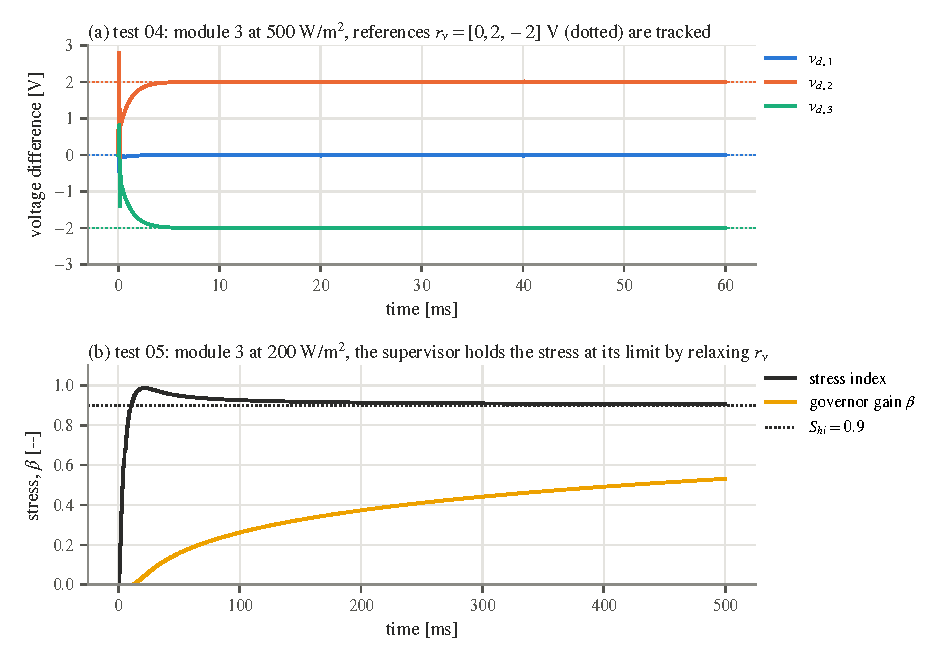
\includegraphics[width=\linewidth]{results/mil_validate}
  \caption[{Two of the MIL validation tests}]{Two of the MIL validation tests: (a) tracking non-zero references under shade, (b) deep shade, where the feasibility governor raises $\beta$ to relax the references and keep the shuffler inside its current rating.}
  \label{fig:mil_validate}
\end{figure}

\begin{figure}[htbp]
  \centering
  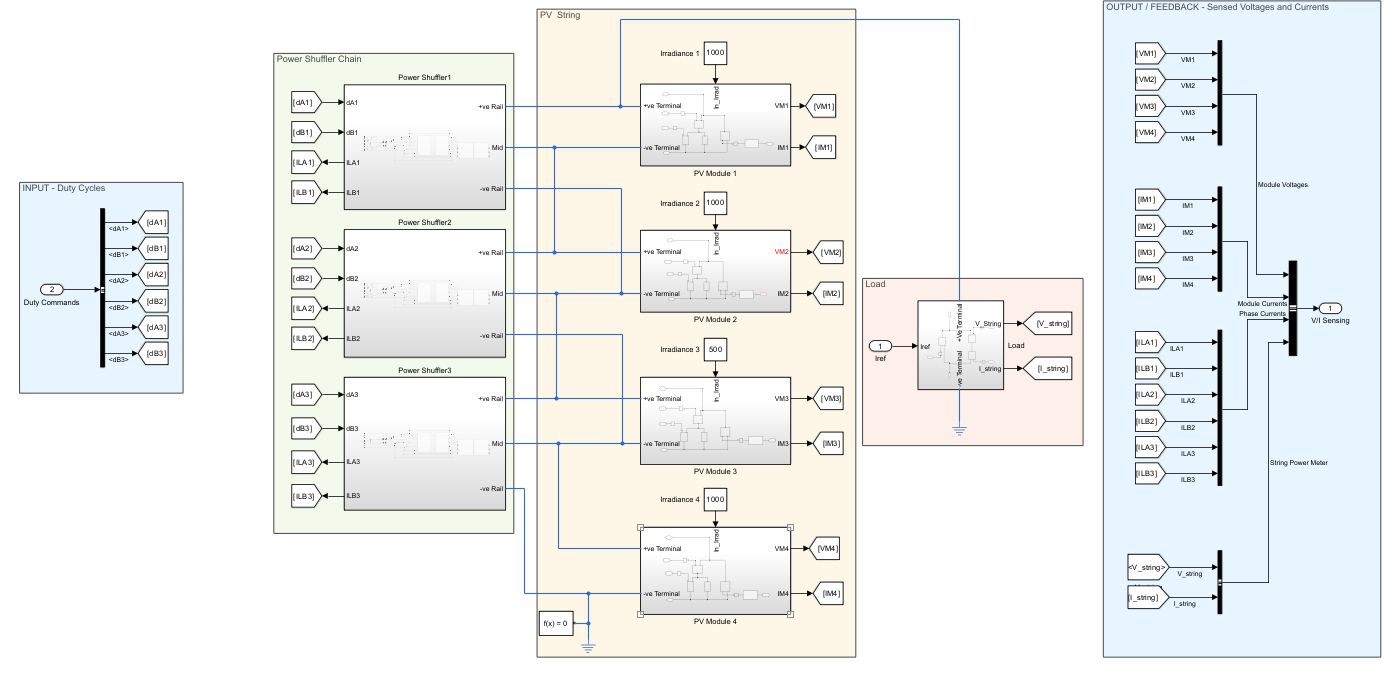
\includegraphics[width=0.92\linewidth]{img-014-016}
  \caption{Inside the MIL plant: four AIKO-class modules and three averaged-switch shufflers.}
  \label{fig:mil_plant}
\end{figure}

\begin{figure}[htbp]
  \centering
  \begin{subfigure}[t]{\linewidth}\centering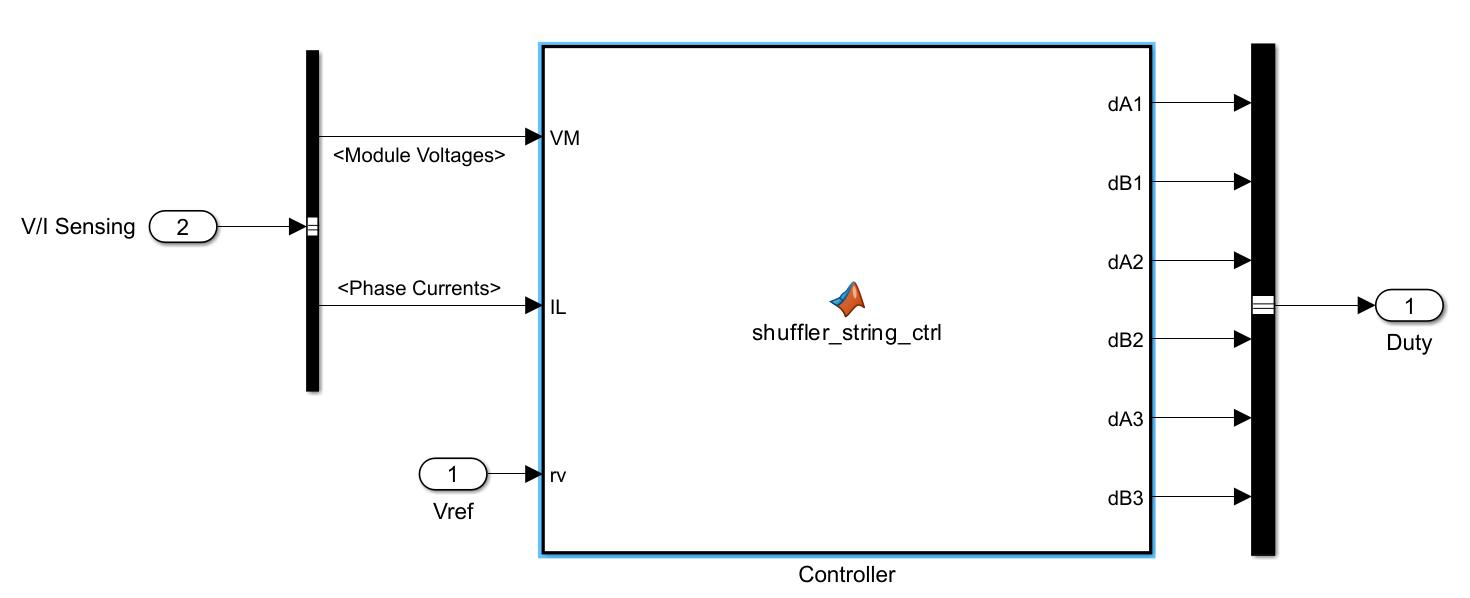
\includegraphics[width=0.9\linewidth]{img-015-017}\caption{Controller block.}\end{subfigure}\\[6pt]
  \begin{subfigure}[t]{\linewidth}\centering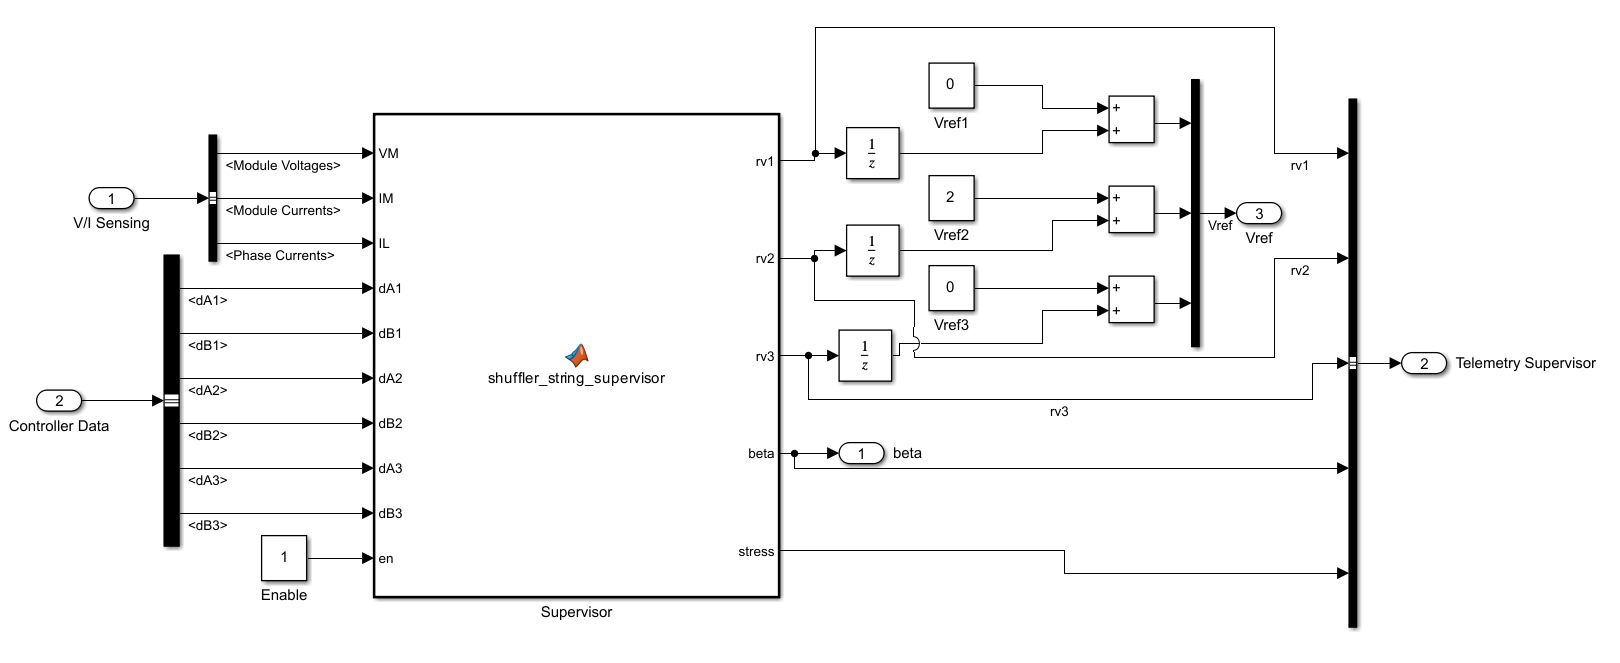
\includegraphics[width=0.9\linewidth]{img-015-018}\caption{Supervisor block.}\end{subfigure}\\[6pt]
  \begin{subfigure}[t]{\linewidth}\centering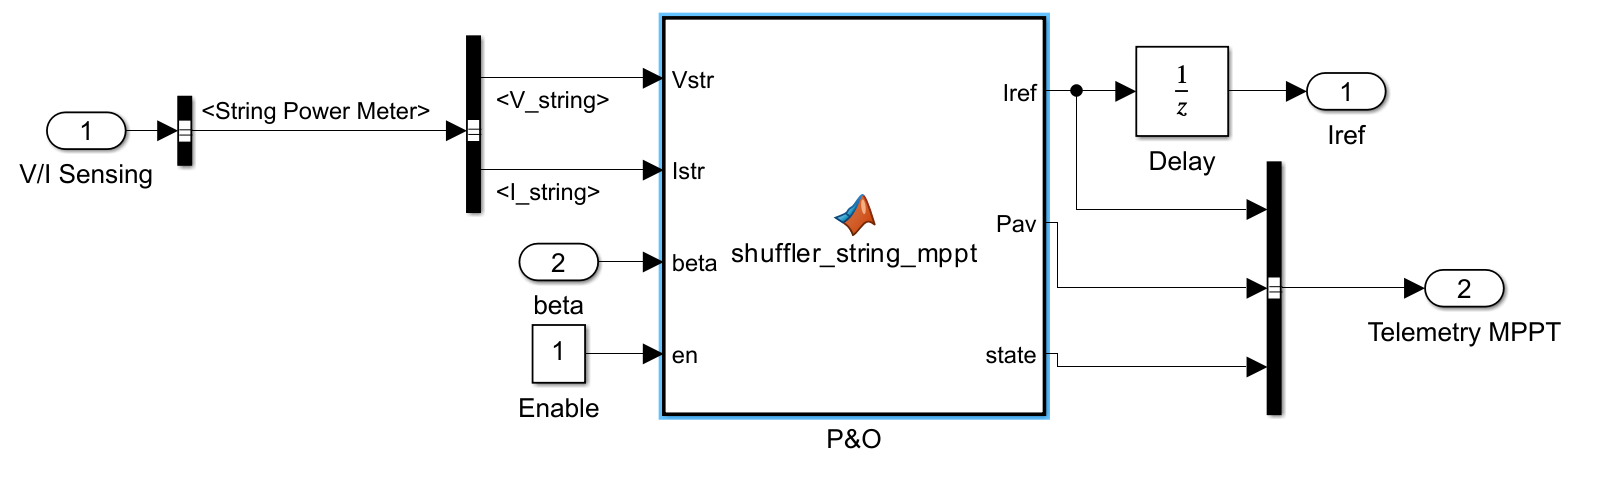
\includegraphics[width=0.9\linewidth]{img-015-019}\caption{MPPT (P\&O) block.}\end{subfigure}
  \caption[{Controller, supervisor and MPPT blocks of the Simulink MIL model}]{The controller, supervisor and MPPT blocks of the Simulink MIL model (\cref{fig:mil}).}
  \label{fig:mil_blocks}
\end{figure}

\section{Simulation Model Sheets}
\label{app:simfigs}
The scenarios run on every model are S1 (loop closure on the open-loop residual), S3 (module 3 loses a third of its current), S4 ($+1\V$ step on the $\vd{}_{,2}$ reference) and S5 (the open-loop duty steps as sent on the bench), each at $k = 0.1$, 0.2, 0.3, 0.5 and 1 on the bench and solar plants: 28 analytical, 25 QSPICE and 25 carpark-twin runs. Their metrics are in \cref{app:synth}; \cref{fig:twin_sim,fig:qspice_run} show representative runs, and all figures are regenerated by \code{make all} in \code{8\_Results/analysis}.

\begin{figure}[htbp]
  \centering
  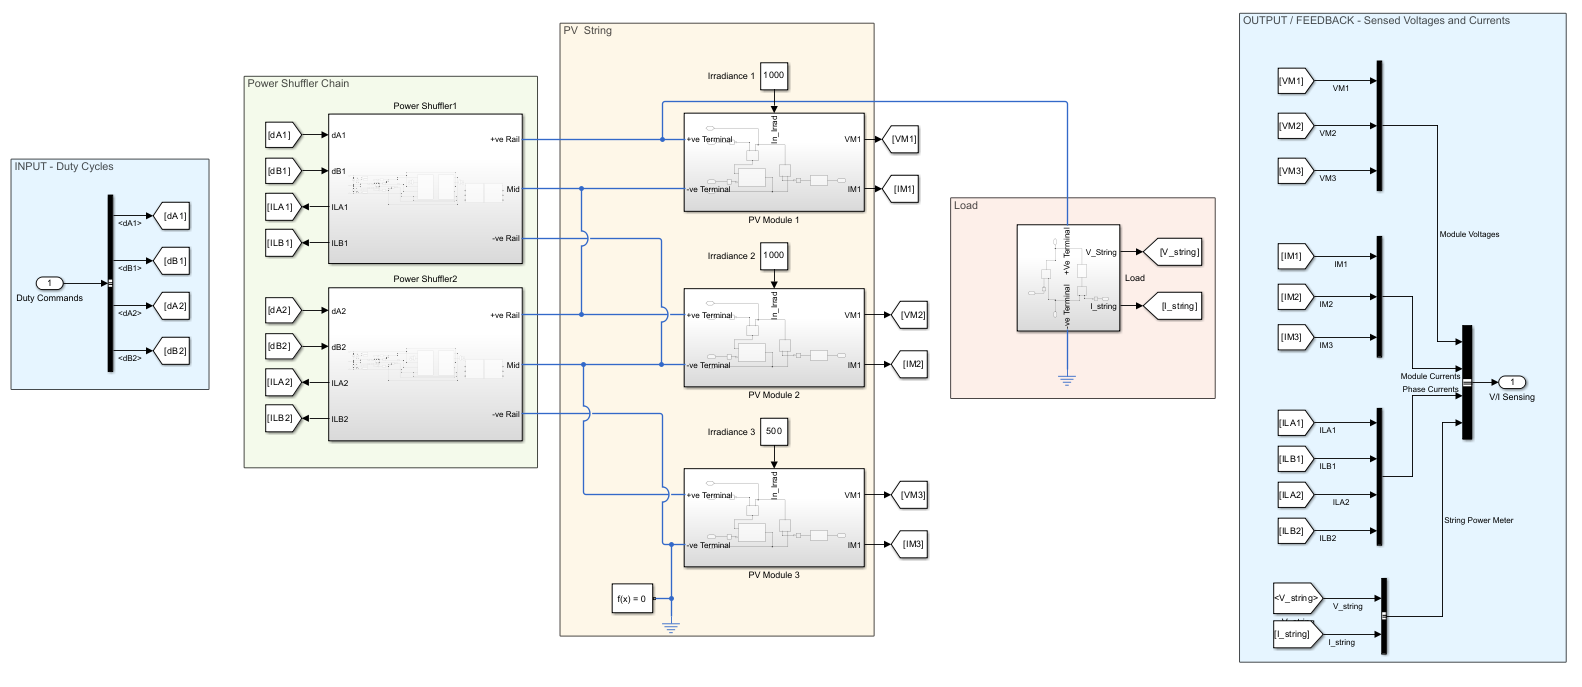
\includegraphics[width=0.95\linewidth]{img-020-036}
  \caption[{Simulink carpark twin}]{Simulink carpark twin: three modules, two averaged-switch shufflers, the sensing block (noise and delay) and the DL3021 CV load. The power-source and load variants are in \cref{fig:twin_variants}.}
  \label{fig:twin}
\end{figure}

\begin{figure}[htbp]
  \centering
  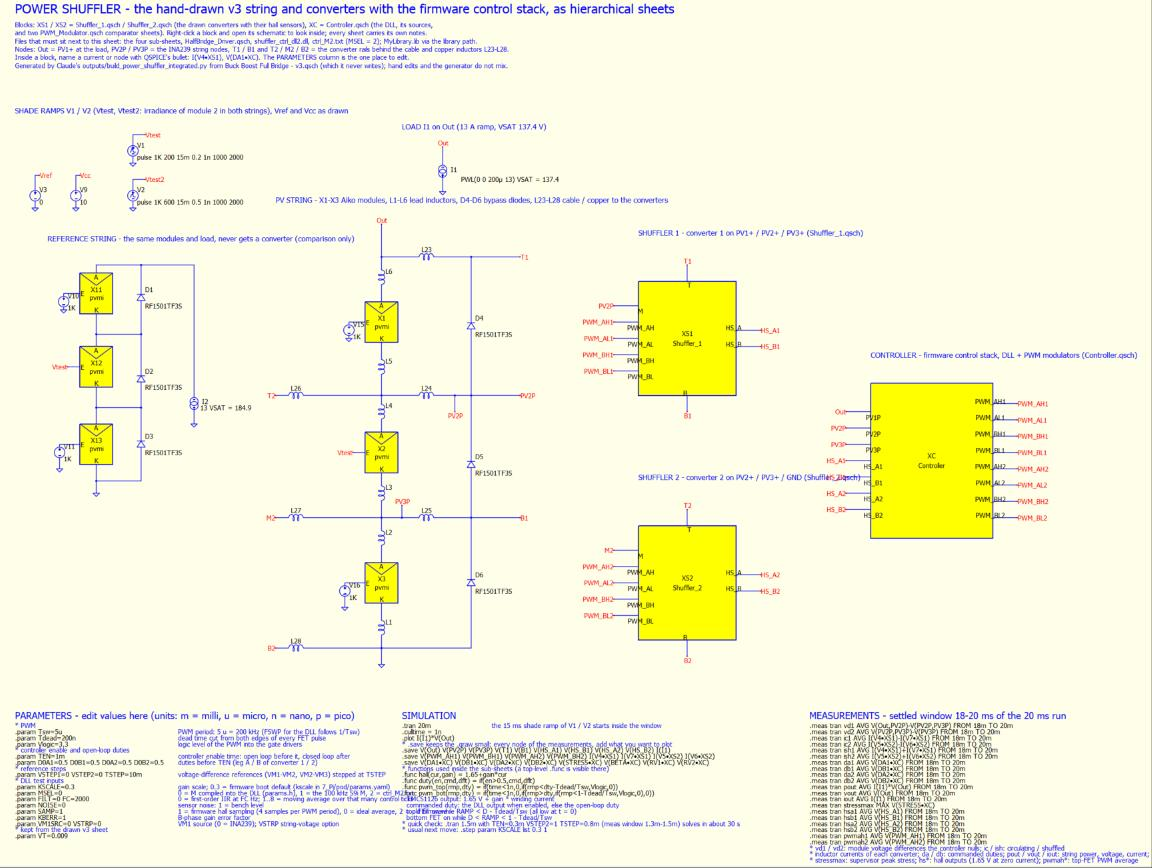
\includegraphics[width=0.8\linewidth]{img-021-041}
  \caption[{QSPICE integrated model, top sheet}]{QSPICE integrated model, top sheet: PV string, two shufflers with real switches, drivers and dead time, and the controller. The controller sheet with the firmware DLL is in \cref{fig:qspice_ctrl}.}
  \label{fig:qspice}
\end{figure}

\begin{figure}[htbp]
  \centering
  \begin{subfigure}[b]{0.45\linewidth}\centering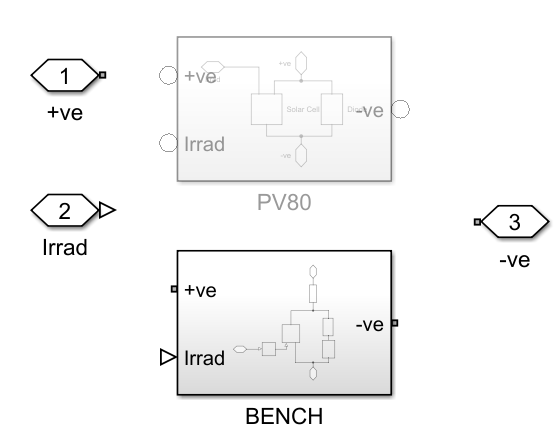
\includegraphics[width=\linewidth]{img-020-038}\caption{Power-source variants (PV80 / BENCH).}\end{subfigure}\hfill
  \begin{subfigure}[b]{0.45\linewidth}\centering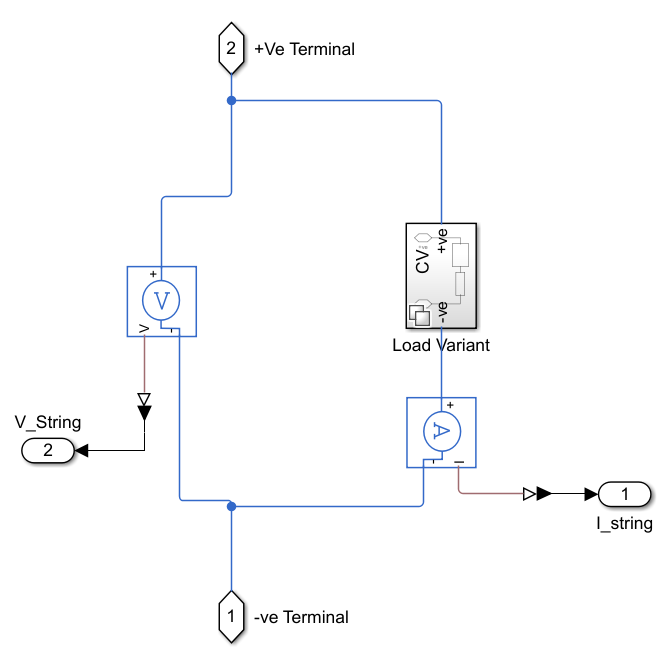
\includegraphics[width=\linewidth]{img-020-039}\caption{Load variants (CV / CC).}\end{subfigure}
  \caption[{Simulink carpark twin: power-source and load variants}]{Simulink carpark twin (\cref{fig:twin}): power-source and load variants.}
  \label{fig:twin_variants}
\end{figure}
\begin{figure}[htbp]
  \centering
  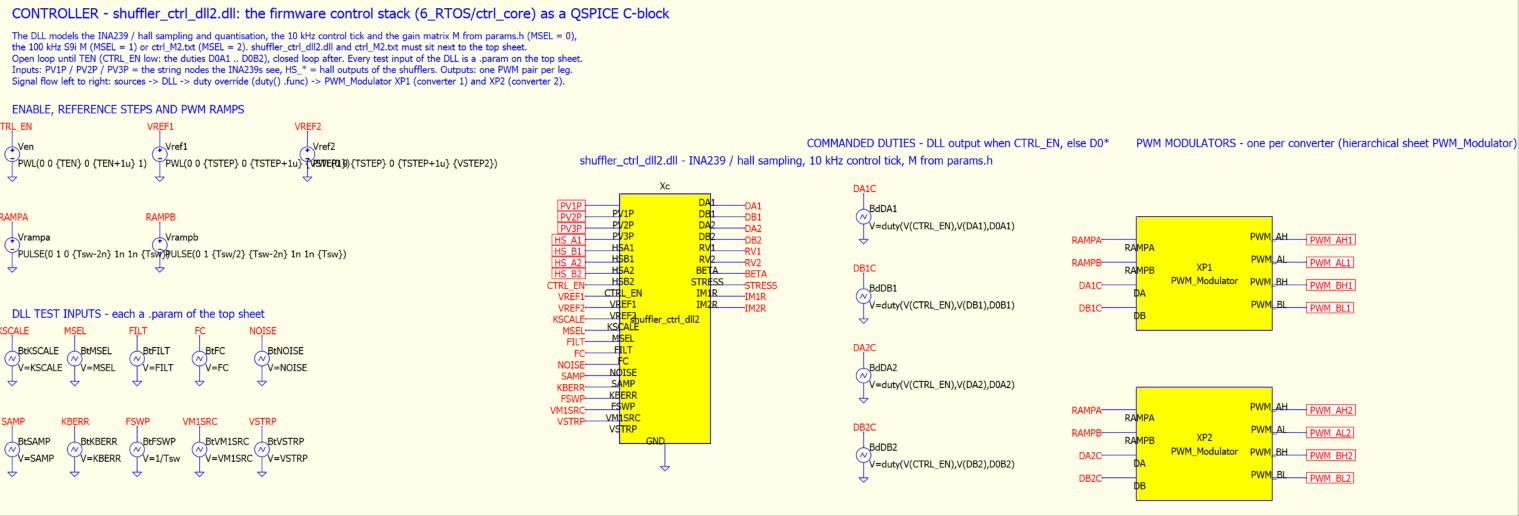
\includegraphics[width=\linewidth]{img-022-045}
  \caption[{QSPICE integrated model, controller sheet}]{QSPICE integrated model (\cref{fig:qspice}), controller sheet: the firmware control DLL (``the Nucleo'') and the HRTIM-style PWM modulators.}
  \label{fig:qspice_ctrl}
\end{figure}

\section{Bench Test Records (16 Oct 2026)}
\label{app:bench}
Ten bench windows were exported from InfluxDB (\cref{tab:T1}); only RUN\_OL and RUN\_CL rows are analysed. The tables below are the evidence behind the open-loop, loop-closure and fault statements of \cref{sec:bench}; the per-window overview and event figures are regenerated by the results pipeline (\code{8\_Results/analysis}, \code{make all}).

% generated by tools/make_tables.py -- do not edit by hand
\begin{table}[htbp]\centering
\small
\caption[{Open-loop duty steps on the bench (B01s, 16 Oct, 200\,kHz)}]{Open-loop duty steps on the bench (B01s, 16 Oct, 200\,kHz): both legs of a shuffler were moved together, so $\Delta u_c = 2\Delta d$, and the averaged model predicts $\Delta v_d = -\bar V\Delta u_c$ with $\bar V = 46.6$\,V. Voltages in V.}\label{tab:T3duty}
\begin{tabular}{l l r r r r r r}
\toprule
Time & Leg duties changed & $\Delta u_{c1}$ & $\Delta u_{c2}$ & \makecell[r]{$\Delta v_{d1}$\\pred.} & \makecell[r]{$\Delta v_{d1}$\\meas.} & \makecell[r]{$\Delta v_{d2}$\\pred.} & \makecell[r]{$\Delta v_{d2}$\\meas.} \\
\midrule
15:11:42 & S2 0.49$\rightarrow$0.51 & 0.00 & +0.04 & 0.00 & -0.03 & -1.86 & -1.87 \\
15:13:00 & S1 0.50$\rightarrow$0.49, S2 0.51$\rightarrow$0.50 & -0.02 & -0.02 & +0.93 & +0.91 & +0.93 & +0.94 \\
15:15:15 & S1 0.49$\rightarrow$0.51 & +0.04 & 0.00 & -1.86 & -1.86 & 0.00 & 0.00 \\
\bottomrule
\end{tabular}
\end{table}

% generated by tools/make_tables.py -- do not edit by hand
\begin{table}[htbp]\centering
\scriptsize
\caption[{Open-loop steady state on hardware (duties 0.5)}]{Open-loop steady state on hardware (duties 0.5): the residual $v_d = -R_m i_m$ and the circulating current the loop has to remove.}\label{tab:T2ol}
\begin{tabular}{l r r r r r r r r r r r r}
\toprule
Case & $f_{sw}$ & $T$ [s] & $\bar v_{d1}$ & $\bar v_{d2}$ & $\bar i_{c1}$ & $\bar i_{c2}$ & $\bar i_{d1}$ & $\bar i_{d2}$ & $V_{M1}$ & $V_{M2}$ & $V_{M3}$ & $P_{load}$ [W] \\
\midrule
B01 & 200 & 321 & 0.01 & -0.17 & 0.66 & 3.54 & 0.47 & -2.92 & 23.3 & 23.3 & 23.4 & 67.9 \\
B01 & 200 & 380 & 0.00 & -0.17 & 0.68 & 3.55 & 0.42 & -2.92 & 23.3 & 23.3 & 23.5 & 66.9 \\
B01s & 200 & 409 & 0.24 & 0.05 & 0.46 & 2.62 & 0.77 & -2.03 & 23.5 & 23.3 & 23.2 & 65.6 \\
B05 & 300 & 280 & 0.08 & -0.58 & 0.51 & 0.05 & 0.55 & -0.57 & 23.2 & 23.1 & 23.7 & 69.1 \\
B05 & 300 & 18 & 0.08 & -0.58 & 0.51 & 0.05 & 0.54 & -0.58 & 23.2 & 23.1 & 23.7 & 69.1 \\
B08 & 400 & 149 & 0.23 & -0.94 & 0.34 & 0.12 & 0.32 & -0.19 & 23.2 & 22.9 & 23.9 & 62.9 \\
S01 & 200 & 184 & -0.25 & -0.32 & -0.75 & 0.96 & -2.20 & -0.88 & 20.1 & 20.3 & 20.6 & 67.7 \\
S03 & 200 & 171 & -0.04 & -0.07 & 0.08 & 1.00 & -0.38 & -0.08 & 20.3 & 20.3 & 20.4 & 9.5 \\
\bottomrule
\end{tabular}
\end{table}

% generated by tools/make_tables.py -- do not edit by hand
\begin{table}[htbp]\centering
\scriptsize
\caption{Gain changes applied while the loop was running (\texttt{C,APPLY} during RUN\_CL) and the 300 kHz stability limit (from T1/T3 and the pod command log).}\label{tab:T3kscale}
\begin{tabular}{l l p{5.5cm} p{6cm}}
\toprule
Case & Time & Action & Outcome \\
\midrule
B04 & 16:07:50 & kscale 0.3 $\rightarrow$ 0.4 applied in RUN\_CL & fault 0x10 (module UV) within 1 s \\
B07 & 17:37:56 & kscale 0.5 $\rightarrow$ 0.6 applied in RUN\_CL & fault 0x2000 (main-loop stall) within 2 s \\
B07 & 17:38:34 & kscale 0.6 run (6 s) & oscillation: $\sigma(v_{d2})$ 1.41 V, pk-pk 11.8 V, 3.2 Hz aliased \\
B07 & 17:39:41 & kscale 0.6 $\rightarrow$ 0.3 applied in RUN\_CL & fault 0x2000 (main-loop stall) within 2 s \\
B08 & 18:03:40 & PSU change + gain set 400 kHz & OC fault 0x01, restarted \\
\bottomrule
\end{tabular}
\end{table}

% generated by tools/make_tables.py -- do not edit by hand
{\scriptsize
\begin{longtable}{l l r l r r r r l r r}
\caption[{Loop closures on hardware (IDLE $\rightarrow$ SOFTSTART $\rightarrow$ RUN\_CL)}]{Loop closures on hardware (IDLE $\rightarrow$ SOFTSTART $\rightarrow$ RUN\_CL): the residual left by the 150\,ms soft-start ramp and how the loop removes it. $t_{s,abs}$ is the time to stay inside $\pm 0.1$\,V / $\pm 0.2$\,A.}\label{tab:T3close}\\
\toprule
Case & Time & $k$ & Signal & IDLE level & $y$ at RUN\_CL & $y_\infty$ & SSE & Rise & $t_{s,abs}$ [s] & Noise \\
\midrule\endfirsthead
\toprule
Case & Time & $k$ & Signal & IDLE level & $y$ at RUN\_CL & $y_\infty$ & SSE & Rise & $t_{s,abs}$ [s] & Noise \\
\midrule\endhead
\bottomrule\endfoot
B02 & 15:31:37 & 0.1 & vd2 & -4.97 & -0.01 & 0.000 & 0.000 & - & 0.00 & 0.030 \\
B02 & 15:31:37 & 0.1 & ic2 & 0.01 & 1.58 & -0.399 & -0.399 & $\leq$ 89 ms & 2.84 & 0.980 \\
B02 & 15:34:19 & 0.1 & vd2 & -4.95 & 0.06 & 0.000 & 0.000 & - & 0.00 & 0.015 \\
B02 & 15:34:19 & 0.1 & ic2 & 0.03 & -0.98 & -0.458 & -0.458 & $\leq$ 88 ms & 2.91 & 1.629 \\
B03 & 16:02:08 & 0.3 & vd2 & -4.95 & -0.09 & 0.015 & 0.015 & $\leq$ 71 ms & 1.90 & 0.044 \\
B03 & 16:02:08 & 0.3 & ic2 & 0.01 & 0.10 & 0.158 & 0.158 & - & 2.99 & 0.528 \\
B04 & 16:07:03 & 0.3 & vd2 & -4.95 & -0.07 & 0.030 & 0.030 & - & 1.48 & 0.044 \\
B04 & 16:07:03 & 0.3 & ic2 & -0.00 & -0.07 & -0.116 & -0.116 & - & 2.99 & 0.586 \\
B06 & 17:17:01 & 0.3 & vd2 & -4.98 & -0.21 & 0.000 & 0.000 & $\leq$ 23 ms & 0.00 & 0.000 \\
B06 & 17:17:01 & 0.3 & ic2 & -0.02 & -0.04 & -0.012 & -0.012 & - & 0.00 & 0.056 \\
B06 & 17:23:14 & 0.3 & vd2 & -4.98 & -0.13 & 0.000 & 0.000 & $\leq$ 23 ms & 0.00 & 0.015 \\
B06 & 17:23:14 & 0.3 & ic2 & -0.01 & -0.01 & -0.015 & -0.015 & - & 0.00 & 0.066 \\
B07 & 17:37:20 & 0.5 & vd2 & -4.96 & -0.19 & 0.010 & 0.010 & $\leq$ 23 ms & 2.69 & 0.074 \\
B07 & 17:37:20 & 0.5 & ic2 & -0.02 & -0.04 & 0.007 & 0.007 & - & 0.00 & 0.063 \\
B07 & 17:38:34 & 0.6 & vd2 & -4.96 & -0.20 & 0.035 & 0.035 & $\leq$ 23 ms & 2.51 & 0.037 \\
B07 & 17:38:34 & 0.6 & ic2 & -0.01 & -0.04 & -0.002 & -0.002 & - & 1.26 & 0.044 \\
B07 & 17:39:20 & 0.4 & vd2 & -4.94 & -0.19 & -0.010 & -0.010 & $\leq$ 23 ms & 0.00 & 0.059 \\
B07 & 17:39:20 & 0.4 & ic2 & -0.02 & -0.05 & -0.019 & -0.019 & - & 0.00 & 0.062 \\
B07 & 17:40:07 & 0.3 & vd2 & -4.95 & -0.20 & 0.000 & 0.000 & $\leq$ 23 ms & 0.00 & 0.015 \\
B07 & 17:40:07 & 0.3 & ic2 & -0.01 & -0.02 & 0.008 & 0.008 & - & 0.00 & 0.061 \\
B09 & 18:05:20 & 0.3 & vd2 & -4.96 & -0.46 & 0.000 & 0.000 & $\leq$ 23 ms & 0.00 & 0.015 \\
B09 & 18:05:20 & 0.3 & ic2 & 0.02 & 0.06 & 0.082 & 0.082 & - & 0.73 & 0.091 \\
B09 & 18:07:37 & 0.3 & vd2 & -4.97 & -0.80 & 0.000 & 0.000 & $\leq$ 23 ms & 0.00 & 0.015 \\
B09 & 18:07:37 & 0.3 & ic2 & 0.02 & 0.14 & 0.049 & 0.049 & - & 1.85 & 0.068 \\
B09 & 18:08:24 & 0.3 & vd2 & -4.96 & -0.17 & 0.010 & 0.010 & $\leq$ 23 ms & 0.00 & 0.015 \\
B09 & 18:08:24 & 0.3 & ic2 & 0.01 & 0.10 & 0.048 & 0.048 & - & 2.49 & 0.068 \\
B09 & 18:12:32 & 0.3 & vd2 & -4.96 & -0.80 & -0.010 & -0.010 & $\leq$ 23 ms & 0.18 & 0.015 \\
B09 & 18:12:32 & 0.3 & ic2 & 0.01 & 0.08 & 0.050 & 0.050 & - & 1.48 & 0.087 \\
S02 & 15:08:45 & 0.1 & vd2 & 0.00 & -0.17 & 0.000 & 0.000 & $\leq$ 43 ms & 0.00 & 0.015 \\
S02 & 15:08:45 & 0.1 & ic2 & -0.03 & 0.29 & -0.049 & -0.049 & $\leq$ 40 ms & 2.97 & 0.305 \\
S04 & 15:52:05 & 0.1 & vd2 & -0.03 & 0.13 & 0.000 & 0.000 & $\leq$ 23 ms & 3.00 & 0.119 \\
S04 & 15:52:05 & 0.1 & ic2 & -0.05 & 0.30 & 0.070 & 0.070 & - & 3.00 & 0.326 \\
S05 & 15:56:54 & 0.2 & vd2 & -0.01 & -0.26 & -0.030 & -0.030 & $\leq$ 37 ms & 2.99 & 0.119 \\
S05 & 15:56:54 & 0.2 & ic2 & -0.04 & 0.34 & -0.023 & -0.023 & $\leq$ 23 ms & 2.97 & 0.245 \\
S06 & 16:01:08 & 0.3 & vd2 & -0.02 & -0.17 & -0.015 & -0.015 & $\leq$ 23 ms & 2.91 & 0.037 \\
S06 & 16:01:08 & 0.3 & ic2 & -0.04 & -0.03 & -0.154 & -0.154 & - & 2.99 & 0.302 \\
S07 & 16:05:37 & 0.4 & vd2 & -0.03 & -0.03 & -0.030 & -0.030 & - & 2.91 & 0.052 \\
S07 & 16:05:37 & 0.4 & ic2 & -0.03 & 0.53 & -0.226 & -0.226 & $\leq$ 23 ms & 2.97 & 0.270 \\
S08 & 16:09:44 & 0.5 & vd2 & -0.03 & -0.13 & 0.010 & 0.010 & $\leq$ 23 ms & 2.66 & 0.059 \\
S08 & 16:09:44 & 0.5 & ic2 & -0.04 & 0.06 & -0.027 & -0.027 & - & 2.97 & 0.412 \\
S09 & 16:13:19 & 0.6 & vd2 & -0.03 & -0.15 & -0.010 & -0.010 & $\leq$ 23 ms & 2.86 & 0.089 \\
S09 & 16:13:19 & 0.6 & ic2 & -0.04 & -0.01 & -0.182 & -0.182 & - & 2.99 & 0.386 \\
S10 & 16:19:11 & 0.7 & vd2 & -0.03 & 0.07 & -0.015 & -0.015 & - & 2.77 & 0.104 \\
S10 & 16:19:11 & 0.7 & ic2 & -0.05 & -0.03 & -0.006 & -0.006 & - & 2.97 & 0.178 \\
S11 & 16:23:11 & 0.8 & vd2 & -0.06 & 0.00 & -0.010 & -0.010 & - & 2.80 & 0.052 \\
S11 & 16:23:11 & 0.8 & ic2 & -0.04 & 0.22 & -0.099 & -0.099 & 37.2 ms & 3.00 & 0.279 \\
\end{longtable}}


\section{Solar Test Records (20 Oct 2026)}
\label{app:solar}
Carpark string of three KAUSSP80 modules into the DL3021 at 61\,V CV, 200\,kHz. Peak sun 15:04--15:13 (S01 open loop, S02 closed loop $k=0.1$), minimal sun from 15:48 (S03 open loop, S04--S11 closed loop, $k = 0.1$ to 0.8). Module currents are reconstructed by KCL from the winding currents, duties and the e-load current.

% generated by tools/make_tables.py -- do not edit by hand
{\scriptsize
\begin{longtable}{l l r r r r r r r r r r r r}
\caption[{Power and energy in the solar test windows (20 Oct 2026)}]{Solar test (20 Oct 2026, KAUSSP80 string into a 61\,V CV load): powers in W, module currents in A (KCL reconstruction), energy delivered and energy returned above a weakest-module-limited string.}\label{tab:T7solar}\\
\toprule
Case & Loop & $k$ & $T$ [s] & $\bar P_{load}$ & $\bar P_{shuf}$ & $\bar P_{ret}$ & $P_{ret,max}$ & $I_{M1}$ & $I_{M2}$ & $I_{M3}$ & $E_{load}$ [Wh] & $E_{ret}$ [Wh] & $\eta$ [\%] \\
\midrule\endfirsthead
\toprule
Case & Loop & $k$ & $T$ [s] & $\bar P_{load}$ & $\bar P_{shuf}$ & $\bar P_{ret}$ & $P_{ret,max}$ & $I_{M1}$ & $I_{M2}$ & $I_{M3}$ & $E_{load}$ [Wh] & $E_{ret}$ [Wh] & $\eta$ [\%] \\
\midrule\endhead
\bottomrule\endfoot
S01 & OL & -- & 188 & 67.3 & 62.3 & 65.9 & 96.1 & 0.00 & 1.76 & 1.54 & 3.51 & 3.44 & 99.3 \\
S02 & CL & 0.1 & 238 & 45.1 & 42.3 & 43.9 & 98.9 & -0.00 & 1.21 & 1.03 & 2.98 & 2.90 & 99.2 \\
S03 & OL & -- & 175 & 9.4 & 9.3 & 9.3 & 11.1 & -0.04 & 0.31 & 0.19 & 0.46 & 0.45 & 99.9 \\
S04 & CL & 0.1 & 266 & 8.2 & 8.2 & 8.0 & 9.0 & -0.04 & 0.28 & 0.16 & 0.60 & 0.59 & 99.9 \\
S05 & CL & 0.2 & 230 & 10.9 & 10.6 & 10.7 & 12.4 & -0.04 & 0.35 & 0.22 & 0.69 & 0.68 & 99.9 \\
S06 & CL & 0.3 & 189 & 13.4 & 12.5 & 13.1 & 14.2 & -0.03 & 0.42 & 0.27 & 0.70 & 0.69 & 99.9 \\
S07 & CL & 0.4 & 156 & 13.5 & 13.0 & 13.3 & 14.2 & -0.04 & 0.42 & 0.28 & 0.59 & 0.58 & 99.9 \\
S08 & CL & 0.5 & 151 & 10.6 & 10.6 & 10.4 & 11.8 & -0.04 & 0.34 & 0.22 & 0.44 & 0.44 & 99.9 \\
S09 & CL & 0.6 & 279 & 7.3 & 7.3 & 7.2 & 8.5 & -0.04 & 0.27 & 0.13 & 0.57 & 0.55 & 100.0 \\
S10 & CL & 0.7 & 179 & 5.1 & 5.8 & 5.0 & 6.1 & -0.04 & 0.21 & 0.09 & 0.26 & 0.25 & 100.1 \\
S11 & CL & 0.8 & 91 & 2.3 & 4.4 & 2.3 & 3.2 & -0.06 & 0.14 & 0.03 & 0.06 & 0.06 & 100.3 \\
\end{longtable}}
\noindent{\footnotesize Module 1 carried $\approx 0$\,A in every window, so a plain series string would have delivered nothing to a 61\,V load: $E_{ret} \approx E_{load}$.}

% generated by tools/make_tables.py -- do not edit by hand
{\scriptsize
\begin{longtable}{l l l l r r r r r}
\caption{Detected shade / irradiance events in the 20 Oct solar windows (current-mismatch and string-power level shifts; irradiance was not logged).}\label{tab:T3shade}\\
\toprule
Case & Event & Time & Signal & $y_0$ & $y_\infty$ & $\Delta$ & Peak dev. & $t_{s,2\%}$ [s] \\
\midrule\endfirsthead
\toprule
Case & Event & Time & Signal & $y_0$ & $y_\infty$ & $\Delta$ & Peak dev. & $t_{s,2\%}$ [s] \\
\midrule\endhead
\bottomrule\endfoot
S01 & mismatch\_off & 15:07:31 & id2 & -0.62 & -0.20 & 0.42 & -- & 0.66 \\
S01 & mismatch\_off & 15:07:31 & vd2 & -0.25 & -0.11 & 0.14 & -- & 2.93 \\
S01 & mismatch\_off & 15:07:31 & Pstr\_i & 53.35 & 18.40 & -34.95 & -- & 4.89 \\
S01 & mismatch\_off & 15:07:31 & IM3 & 1.18 & 0.41 & -0.77 & -- & 4.14 \\
S01 & irradiance\_down & 15:07:32 & Pstr\_i & 51.23 & 18.39 & -32.83 & -- & 1.84 \\
S01 & irradiance\_down & 15:07:32 & id2 & -0.61 & -0.21 & 0.39 & -- & 0.00 \\
S01 & irradiance\_down & 15:07:32 & vd2 & -0.24 & -0.11 & 0.13 & -- & 1.93 \\
S02 & mismatch\_on & 15:09:24 & id2 & -0.57 & -1.44 & -0.87 & -- & 4.56 \\
S02 & mismatch\_on & 15:09:24 & vd2 & 0.00 & 0.00 & 0.00 & 0.06 & 0.00 \\
S02 & mismatch\_on & 15:09:24 & Pstr\_i & 42.20 & 98.24 & 56.04 & -- & 5.92 \\
S02 & mismatch\_on & 15:09:24 & IM3 & 0.97 & 2.33 & 1.35 & -- & 7.51 \\
S02 & irradiance\_up & 15:09:24 & Pstr\_i & 42.20 & 98.24 & 56.04 & -- & 5.92 \\
S02 & irradiance\_up & 15:09:24 & id2 & -0.57 & -1.44 & -0.87 & -- & 4.56 \\
S02 & irradiance\_up & 15:09:24 & vd2 & 0.00 & 0.00 & 0.00 & 0.06 & 0.00 \\
S02 & irradiance\_down & 15:10:29 & Pstr\_i & 86.29 & 53.38 & -32.91 & -- & 0.00 \\
S02 & irradiance\_down & 15:10:29 & id2 & -1.20 & -0.71 & 0.50 & -- & 0.00 \\
S02 & irradiance\_down & 15:10:29 & vd2 & 0.00 & 0.00 & 0.00 & -0.05 & 0.00 \\
S02 & mismatch\_off & 15:10:31 & id2 & -1.04 & -0.60 & 0.44 & -- & 11.40 \\
S02 & mismatch\_off & 15:10:31 & vd2 & 0.00 & 0.00 & 0.00 & 0.05 & 0.00 \\
S02 & mismatch\_off & 15:10:31 & Pstr\_i & 75.64 & 47.10 & -28.54 & -- & 0.00 \\
S02 & mismatch\_off & 15:10:31 & IM3 & 1.78 & 1.05 & -0.73 & -- & 0.00 \\
S02 & mismatch\_on & 15:10:40 & id2 & -0.55 & -0.33 & 0.22 & -1.02 & 7.31 \\
S02 & mismatch\_on & 15:10:40 & vd2 & 0.00 & 0.00 & 0.00 & 0.05 & 0.00 \\
S02 & mismatch\_on & 15:10:40 & Pstr\_i & 42.57 & 30.44 & -12.13 & -- & 11.70 \\
S02 & mismatch\_on & 15:10:40 & IM3 & 0.98 & 0.67 & -0.31 & -- & 9.95 \\
S02 & mismatch\_off & 15:10:48 & id2 & -0.79 & -0.38 & 0.42 & -- & 0.00 \\
S02 & mismatch\_off & 15:10:48 & vd2 & 0.00 & 0.00 & 0.00 & 0.05 & 0.00 \\
S02 & mismatch\_off & 15:10:48 & Pstr\_i & 56.71 & 32.50 & -24.21 & -- & 2.69 \\
S02 & mismatch\_off & 15:10:48 & IM3 & 1.30 & 0.71 & -0.59 & -- & 1.93 \\
S03 & mismatch\_on & 15:48:53 & id2 & -0.10 & -0.10 & -0.00 & -0.61 & 0.00 \\
S03 & mismatch\_on & 15:48:53 & vd2 & -0.07 & -0.07 & 0.00 & -0.26 & 18.03 \\
S03 & mismatch\_on & 15:48:53 & Pstr\_i & 10.43 & 10.00 & -0.43 & 0.62 & 0.00 \\
S03 & mismatch\_on & 15:48:53 & IM3 & 0.22 & 0.22 & -0.01 & 0.30 & 0.00 \\
S03 & mismatch\_off & 15:48:59 & id2 & -0.11 & -0.12 & -0.01 & 0.63 & 0.00 \\
S03 & mismatch\_off & 15:48:59 & vd2 & -0.07 & -0.07 & 0.00 & -0.26 & 0.75 \\
S03 & mismatch\_off & 15:48:59 & Pstr\_i & 10.35 & 9.88 & -0.47 & 0.55 & 0.00 \\
S03 & mismatch\_off & 15:48:59 & IM3 & 0.22 & 0.22 & -0.00 & -0.32 & 0.00 \\
S03 & mismatch\_off & 15:49:18 & id2 & -0.11 & -0.11 & 0.00 & 0.62 & 0.00 \\
S03 & mismatch\_off & 15:49:18 & vd2 & -0.07 & -0.07 & 0.00 & 0.24 & 8.93 \\
S03 & mismatch\_off & 15:49:18 & Pstr\_i & 9.90 & 9.60 & -0.30 & 0.36 & 0.00 \\
S03 & mismatch\_off & 15:49:18 & IM3 & 0.22 & 0.21 & -0.01 & -0.31 & 0.00 \\
S05 & mismatch\_on & 15:58:21 & id2 & -0.10 & -0.06 & 0.04 & 0.71 & 19.36 \\
S05 & mismatch\_on & 15:58:21 & vd2 & 0.00 & -0.00 & -0.00 & -0.25 & 14.98 \\
S05 & mismatch\_on & 15:58:21 & Pstr\_i & 10.45 & 10.86 & 0.42 & -0.72 & 0.00 \\
S05 & mismatch\_on & 15:58:21 & IM3 & 0.22 & 0.21 & -0.01 & -0.36 & 19.36 \\
S08 & mismatch\_on & 16:10:42 & id2 & -0.08 & -0.07 & 0.01 & -0.64 & 0.00 \\
S08 & mismatch\_on & 16:10:42 & vd2 & 0.01 & -0.01 & -0.02 & 0.22 & 17.23 \\
S08 & mismatch\_on & 16:10:42 & Pstr\_i & 11.12 & 10.73 & -0.39 & 0.57 & 0.00 \\
S08 & mismatch\_on & 16:10:42 & IM3 & 0.22 & 0.21 & -0.01 & 0.32 & 0.00 \\
\end{longtable}}


\section{Synthesis: Inventory and Metrics}
\label{app:synth}
{\sloppy All tables are generated from the pipeline CSVs (\code{8\_Results/analysis/out/tables}) by \code{tools/make\_tables.py}; \code{make all} in \code{8\_Results/analysis} rebuilds the CSVs from the exported test windows (the full set, including every event and every signal, is in \code{REPORT.md} and the CSVs). Only the tables the report cites are reproduced here.\par}

\subsection{Metric definitions}
Every metric has one definition for every phase (\code{stepmetrics.py}): initial and final levels (medians), step size, 10--90\,\% rise time, peak value and time, overshoot and undershoot, 2\,\%, 5\,\% and absolute-band settling times, steady-state error, IAE, and a fitted $\tau$ or $(\zeta, \omega_n)$. Noise is the median absolute deviation of the pre-event window; steady state is reported as mean, standard deviation, peak-to-peak, RMS and dominant frequency (Welch); and energy as $E_{load}$, $E_{shuffled}$ and $E_{returned} = \int (I_{str} - \max(\min_k I_k, 0))\,V_{str}\,\mathrm{d}t$.

\subsection{Test-case inventory and data rules}
% generated by tools/make_tables.py -- do not edit by hand
{\scriptsize
\begin{longtable}{l l l r l l l r r p{3.4cm}}
\caption[{Test-case inventory}]{Test-case inventory: the raw-data slide windows re-exported from the pod's InfluxDB (RUN\_OL / RUN\_CL rows only).}\label{tab:T1}\\
\toprule
Case & Slide & Setup & $f_{sw}$ [kHz] & Loop & $k$ & Window (AEST) & RUN [s] & Rate [Hz] & Note \\
\midrule\endfirsthead
\toprule
Case & Slide & Setup & $f_{sw}$ [kHz] & Loop & $k$ & Window (AEST) & RUN [s] & Rate [Hz] & Note \\
\midrule\endhead
\bottomrule\endfoot
B01 & p48 & BENCH & 200 & OL & -- & 14:32:00-14:44:56 & 706 & 40 & duties 0.5; e-load CV set-point steps 125 <$\rightarrow$ 60 V; VM1 from \\
B01s &  & BENCH & 200 & OL & -- & 15:09:00-15:16:00 & 412 & 40 & not on a slide: the only open-loop duty steps (15:11:42 S2 + \\
B02 & p42 & BENCH & 200 & CL & 0.1 & 15:31:34-15:34:25 & 161 & 11 & before the ADC fix; PSU unstable \\
B03 & p43 & BENCH & 200 & CL & 0.3 & 16:02:05-16:04:33 & 143 & 14 & slide says kscale 20 \%, telemetry says 0.3 with pset 0 (boot \\
B04 & p44 & BENCH & 200 & CL & 0.3/0.4 & 16:07:00-16:07:49 & 47 & 14 & kscale 0.4 applied at 16:07:50 $\rightarrow$ OC fault within 1 s \\
B05 & p49 & BENCH & 300 & OL & -- & 16:31:36-16:37:04 & 304 & 36 & nan \\
B06 & p45 & BENCH & 300 & CL & 0.3 & 17:17:00-17:25:49 & 512 & 44 & PSU / e-load set-point steps 17:22:30-17:25:30 while closed \\
B07 & p46 & BENCH & 300 & CL & 0.3/0.4/0.5/0.6 & 17:34:08-17:41:47 & 295 & 44 & nan \\
B08 & p50 & BENCH & 400 & OL & -- & 18:02:03-18:04:38 & 152 & 44 & PSU change at 18:03:40 \\
B09 & p47 & BENCH & 400 & CL & 0.3 & 18:05:11-18:13:40 & 392 & 44 & nan \\
S01 & p24 & PV80 & 200 & OL & -- & 15:04:35-15:07:47 & 187 & 44 & peak sun \\
S02 & p25 & PV80 & 200 & CL & 0.1 & 15:08:40-15:12:44 & 237 & 44 & peak sun; shade event about 15:09:20-15:10:40 \\
S03 & p26 & PV80 & 200 & OL & -- & 15:48:22-15:51:20 & 174 & 44 & minimal sun \\
S04 & p27 & PV80 & 200 & CL & 0.1 & 15:52:03-15:56:31 & 265 & 44 & minimal sun \\
S05 & p37 & PV80 & 200 & CL & 0.2 & 15:56:51-16:00:47 & 229 & 44 & minimal sun \\
S06 & p38 & PV80 & 200 & CL & 0.3 & 16:01:07-16:04:19 & 189 & 44 & minimal sun \\
S07 & p39 & PV80 & 200 & CL & 0.4 & 16:05:30-16:08:17 & 156 & 44 & minimal sun \\
S08 & p40 & PV80 & 200 & CL & 0.5 & 16:09:42-16:12:16 & 150 & 44 & minimal sun \\
S09 &  & PV80 & 200 & CL & 0.6 & 16:13:15-16:18:00 & 278 & 44 & not on a slide (closed\_loop\_timeslots.pdf) \\
S10 &  & PV80 & 200 & CL & 0.7 & 16:19:05-16:22:12 & 178 & 44 & not on a slide (closed\_loop\_timeslots.pdf) \\
S11 &  & PV80 & 200 & CL & 0.8 & 16:23:05-16:24:45 & 90 & 44 & not on a slide (closed\_loop\_timeslots.pdf) \\
\end{longtable}}
\noindent{\footnotesize B01s and S09--S11 are not on a slide. B03 ran at $k=0.3$ (telemetry), not the 20\,\% written on the slide.}

\begin{itemize}
  \item Only RUN\_OL / RUN\_CL frames are analysed; frames repeating all ten control fields are dropped; leading/trailing frames where $V_{M2}$ or $V_{M3}$ left the run median by $>2\V$ (supply switched off before the FAULT) are dropped.
  \item $I_{M1r}$ / $I_{M2r}$ are recomputed from $I_{LA}$, $I_{LB}$, the duties and the e-load current by the firmware's KCL (\cref{lst:recon}): $I_1 = I_{str} + d_{A1}I_{LA1} - d_{B1}I_{LB1}$, $I_3 = I_{str} - (i_{sh2} - d_{A2}I_{LA2} + d_{B2}I_{LB2})$, $I_2 = I_3 + I_{M2r}$.
  \item $V_{M1}$: where the telemetry $V_{M1}$ disagrees with the 5\,Hz e-load by $>2\V$ (200\,kHz open-loop runs) it is replaced by $V_{eload} - V_{M2} - V_{M3}$; $\vd{}_{,2}$ is the primary hardware voltage signal.
  \item Hardware times shorter than one telemetry frame (23\,ms at 44\,Hz; 70--90\,ms at 11--14\,Hz) are bounds, printed ``$\le$''.
\end{itemize}

\subsection{Hardware closed-loop steady state}
% generated by tools/make_tables.py -- do not edit by hand
{\scriptsize
\begin{longtable}{l r r r r r r r r r r r}
\caption[{Closed-loop steady state on hardware (settled RUN\_CL segments $\geq 5$\,s)}]{Closed-loop steady state on hardware (settled RUN\_CL segments $\geq 5$\,s): the references $v_d=0$, $i_c=0$ are held with no measurable offset; $\sigma$ is sample-to-sample sensing noise at 44\,Hz.}\label{tab:T2cl}\\
\toprule
Case & $f_{sw}$ & $k$ & $T$ [s] & $\bar v_{d2}$ [V] & $\sigma(v_{d2})$ & pk-pk & $\bar i_{c2}$ [A] & $\sigma(i_{c2})$ & $\bar i_{d1}$ [A] & $\bar i_{d2}$ [A] & $\bar P_{load}$ [W] \\
\midrule\endfirsthead
\toprule
Case & $f_{sw}$ & $k$ & $T$ [s] & $\bar v_{d2}$ [V] & $\sigma(v_{d2})$ & pk-pk & $\bar i_{c2}$ [A] & $\sigma(i_{c2})$ & $\bar i_{d1}$ [A] & $\bar i_{d2}$ [A] & $\bar P_{load}$ [W] \\
\midrule\endhead
\bottomrule\endfoot
B02 & 200 & 0.1 & 153 & 0.005 & 0.040 & 0.21 & -0.023 & 1.36 & 0.35 & -0.10 & 44.5 \\
B03 & 200 & 0.3 & 140 & 0.007 & 0.074 & 0.36 & 0.050 & 0.40 & 0.09 & -0.05 & 40.6 \\
B04 & 200 & 0.3 & 44 & 0.010 & 0.078 & 0.39 & 0.066 & 0.41 & 0.19 & 0.04 & 40.6 \\
B06 & 300 & 0.3 & 357 & 0.001 & 0.016 & 0.08 & -0.000 & 0.05 & 0.31 & -0.26 & 35.6 \\
B06 & 300 & 0.3 & 148 & 0.001 & 0.016 & 0.08 & -0.000 & 0.05 & 0.70 & -0.49 & 61.7 \\
B07 & 300 & 0.4 & 132 & -0.002 & 0.069 & 0.27 & -0.001 & 0.05 & 0.41 & -0.48 & 61.0 \\
B07 & 300 & 0.5 & 33 & -0.005 & 0.095 & 0.36 & 0.000 & 0.06 & 0.36 & -0.07 & 45.5 \\
B07 & 300 & 0.6 & 6 & 0.052 & 1.406 & 11.81 & 0.004 & 0.06 & 0.19 & -0.21 & 40.6 \\
B07 & 300 & 0.4 & 18 & -0.002 & 0.044 & 0.19 & 0.001 & 0.05 & 0.27 & -0.12 & 45.8 \\
B07 & 300 & 0.3 & 91 & -0.000 & 0.013 & 0.06 & -0.001 & 0.05 & 0.25 & -0.18 & 44.7 \\
B09 & 400 & 0.3 & 96 & 0.001 & 0.015 & 0.08 & 0.057 & 0.09 & 0.21 & -0.09 & 49.8 \\
B09 & 400 & 0.3 & 37 & 0.001 & 0.017 & 0.08 & 0.054 & 0.08 & 0.36 & -0.28 & 63.6 \\
B09 & 400 & 0.3 & 193 & 0.001 & 0.018 & 0.09 & 0.060 & 0.08 & 0.34 & -0.28 & 62.9 \\
B09 & 400 & 0.3 & 55 & -0.003 & 0.035 & 0.16 & 0.061 & 0.09 & 0.36 & -0.27 & 63.7 \\
S02 & 200 & 0.1 & 234 & 0.001 & 0.031 & 0.14 & -0.032 & 0.23 & -1.51 & -0.58 & 45.5 \\
S04 & 200 & 0.1 & 262 & 0.008 & 0.149 & 0.70 & -0.029 & 0.26 & -0.35 & -0.06 & 8.2 \\
S05 & 200 & 0.2 & 226 & 0.001 & 0.108 & 0.56 & -0.033 & 0.27 & -0.44 & -0.08 & 10.9 \\
S06 & 200 & 0.3 & 186 & 0.002 & 0.088 & 0.41 & -0.039 & 0.27 & -0.51 & -0.11 & 13.4 \\
S07 & 200 & 0.4 & 153 & -0.004 & 0.092 & 0.43 & -0.045 & 0.28 & -0.52 & -0.13 & 13.5 \\
S08 & 200 & 0.5 & 147 & -0.002 & 0.114 & 0.62 & -0.030 & 0.29 & -0.43 & -0.10 & 10.6 \\
S09 & 200 & 0.6 & 275 & -0.000 & 0.172 & 0.80 & -0.050 & 0.30 & -0.32 & -0.02 & 7.3 \\
S10 & 200 & 0.7 & 175 & -0.002 & 0.138 & 0.71 & -0.046 & 0.31 & -0.26 & -0.00 & 5.1 \\
S11 & 200 & 0.8 & 88 & -0.000 & 0.099 & 0.59 & -0.048 & 0.31 & -0.19 & 0.02 & 2.3 \\
\end{longtable}}


\subsection{Cross-phase step metrics}
% generated by tools/make_tables.py -- do not edit by hand
\begin{table}[htbp]\centering
\scriptsize
\caption[{$+1$\,V reference step on $v_{d2}$ (S4), 200\,kHz gain set}]{$+1$\,V reference step on $v_{d2}$ (S4), 200\,kHz gain set: fitted time constant $\tau$, 10--90\,\% rise $t_r$ and 2\,\% settling $t_s$ in ms, analytical model $|$ QSPICE switching model with the firmware DLL $|$ Simulink carpark twin. $\tau_{design} = 1/(k\,2\pi\,150\,\mathrm{Hz})$.}\label{tab:T5s4}
\begin{tabular}{l r r | r r r | r r r r | r r r r}
\toprule
Setup & $k$ & $\tau_{design}$ & $\tau$ & $t_r$ & $t_{s}$ & $\tau$ & $t_r$ & $t_{s}$ & OS\,\% & $\tau$ & $t_r$ & $t_{s}$ & OS\,\% \\
\midrule
BENCH & 0.1 & 10.61 & 10.54 & 23.2 & 41.3 & 9.72 & 19.8 & 30.7 & 0.0 & 10.15 & 22.9 & 41.4 & 0.0 \\
BENCH & 0.2 & 5.31 & 5.20 & 11.5 & 20.5 & 4.62 & 10.4 & 18.4 & 0.0 & 4.77 & 11.0 & 19.8 & 0.0 \\
BENCH & 0.3 & 3.54 & 3.42 & 7.6 & 13.6 & 2.84 & 6.5 & 11.9 & 0.0 & 2.97 & 6.9 & 12.4 & 0.0 \\
BENCH & 0.5 & 2.12 & 1.99 & 4.5 & 8.0 & 1.47 & 3.5 & 6.2 & 0.0 & 1.51 & 3.7 & 6.8 & 0.0 \\
BENCH & 1.0 & 1.06 & 0.91 & 2.0 & 3.8 & 0.55 & 1.3 & 2.2 & 0.0 & 0.40 & 0.8 & 2.7 & 8.8 \\
PV80 & 0.1 & 10.61 & 12.90 & 28.4 & 50.6 & 12.40 & 22.5 & 32.1 & 0.0 & 11.64 & 26.0 & 45.5 & 0.0 \\
PV80 & 0.2 & 5.31 & 6.38 & 14.1 & 25.1 & 5.87 & 12.6 & 21.8 & 0.0 & 5.51 & 12.5 & 22.4 & 0.0 \\
PV80 & 0.3 & 3.54 & 4.21 & 9.4 & 16.7 & 3.71 & 8.7 & 15.2 & 0.0 & 3.47 & 8.1 & 14.2 & 0.0 \\
PV80 & 0.5 & 2.12 & 2.47 & 5.5 & 9.9 & 1.94 & 4.6 & 17.0 & 7.5 & 1.83 & 4.5 & 8.0 & 0.0 \\
PV80 & 1.0 & 1.06 & 1.16 & 2.6 & 4.8 & 0.77 & 1.9 & 8.5 & 4.2 & 0.56 & 0.9 & 3.0 & 0.0 \\
\bottomrule
\end{tabular}
\par\smallskip\raggedright{\scriptsize Hardware cannot resolve this transient (one telemetry frame = 23\,ms); its steady-state error and noise are in Table~\ref{tab:T2cl}.}
\end{table}

% generated by tools/make_tables.py -- do not edit by hand
\begin{table}[htbp]\centering
\scriptsize
\caption[{Circulating-current channel $i_{c2}$ during the $+1$\,V $v_{d2}$ reference step (S4, 200\,kHz)}]{Circulating-current channel $i_{c2}$ during the $+1$\,V $v_{d2}$ reference step (S4, 200\,kHz): peak deviation and recovery, i.e.\ the decoupling check (the current loop should barely move).}\label{tab:T5s4i}
\begin{tabular}{l r r r r r r r r r}
\toprule
Setup & $k$ & peak an. [A] & $t_s$ an. [ms] & peak QSP [A] & $t_s$ QSP [ms] & SSE QSP [A] & peak Sim [A] & $t_s$ Sim [ms] & SSE Sim [A] \\
\midrule
BENCH & 0.1 & -0.004 & 0.0 & -0.038 & 0.0 & 0.005 & -0.007 & 0.0 & 0.006 \\
BENCH & 0.2 & -0.004 & 0.0 & -0.033 & 0.0 & 0.005 & -0.019 & 0.0 & 0.007 \\
BENCH & 0.3 & -0.005 & 0.0 & -0.022 & 0.0 & 0.006 & -0.029 & 0.0 & 0.006 \\
BENCH & 0.4 & -0.005 & 0.0 & -- & -- & -- & -- & -- & -- \\
BENCH & 0.5 & -0.005 & 0.0 & -0.030 & 0.0 & 0.007 & -0.026 & 0.0 & 0.010 \\
BENCH & 1.0 & -0.008 & 0.0 & -0.025 & 0.0 & 0.005 & -0.037 & 0.0 & 0.016 \\
PV80 & 0.1 & -0.005 & 0.0 & -0.051 & 0.0 & 0.064 & 0.017 & 0.0 & -0.010 \\
PV80 & 0.2 & -0.005 & 0.0 & -0.049 & 0.0 & 0.057 & 0.015 & 0.0 & -0.010 \\
PV80 & 0.3 & -0.005 & 0.0 & 0.072 & 0.0 & 0.041 & 0.019 & 0.0 & -0.010 \\
PV80 & 0.4 & -0.005 & 0.0 & -- & -- & -- & -- & -- & -- \\
PV80 & 0.5 & -0.005 & 0.0 & -0.106 & 7.0 & 0.075 & 0.018 & 0.0 & -0.007 \\
PV80 & 1.0 & -0.007 & 0.0 & 0.120 & 0.9 & 0.027 & -0.018 & 0.0 & -0.002 \\
\bottomrule
\end{tabular}
\end{table}

% generated by tools/make_tables.py -- do not edit by hand
\begin{table}[htbp]\centering
\scriptsize
\caption[{Shade disturbance (S3: module 3 loses 1/3 of its current, PV80 plant)}]{Shade disturbance (S3: module 3 loses 1/3 of its current, PV80 plant): simulated recovery (ms) against the detected hardware shade events of 20 Oct.}\label{tab:T5s3}
\begin{tabular}{r l r r r r r r r r l}
\toprule
$k$ & Signal & $\tau$ an. & $t_s$ an. & $\tau$ QSP & $t_s$ QSP & OS QSP & $t_s$ Sim & HW $\Delta$ & HW peak & HW cases \\
\midrule
0.1 & Pstr & -- & -- & 0.00 & 6.3 & 6.2 & 0.1 & 21.95 & -- & S02 S02 \\
0.2 & Pstr & -- & -- & 0.00 & 0.1 & 3.9 & 0.1 & -0.01 & -0.05 & S03 S05 \\
0.3 & Pstr & -- & -- & 0.00 & 3.3 & 7.4 & 0.1 & -- & -- & nan \\
0.5 & Pstr & -- & -- & 0.00 & 1.6 & 4.1 & 0.1 & -0.39 & 0.57 & S08 \\
1.0 & Pstr & -- & -- & 0.00 & 0.7 & 6.1 & 0.1 & -- & -- & nan \\
0.1 & id2 & 0.08 & 18.9 & 0.07 & 15.6 & 0.0 & 0.2 & -0.33 & -1.02 & S02 S02 \\
0.2 & id2 & 0.08 & 9.3 & 0.05 & 0.3 & 0.0 & 0.2 & 0.02 & 0.05 & S03 S05 \\
0.3 & id2 & 0.08 & 6.1 & 0.07 & 7.5 & 0.0 & 0.2 & -- & -- & nan \\
0.4 & id2 & 0.08 & 4.5 & -- & -- & -- & -- & -- & -- & nan \\
0.5 & id2 & 0.08 & 3.6 & 0.06 & 3.0 & 0.0 & 0.2 & 0.01 & -0.64 & S08 \\
1.0 & id2 & 0.08 & 1.6 & 0.06 & 0.9 & 0.0 & 0.2 & -- & -- & nan \\
0.1 & vd2 & -- & -- & -- & -- & -- & -- & 0.00 & 0.05 & S02 S02 \\
0.2 & vd2 & -- & -- & 0.01 & 2.0 & 20.5 & -- & -0.00 & -0.25 & S03 S05 \\
0.5 & vd2 & -- & -- & -- & -- & -- & -- & -0.02 & 0.22 & S08 \\
\bottomrule
\end{tabular}
\end{table}


\section{Thermal Data and Oscilloscope Captures}
\label{app:thermal}
On the bench the hottest die rose from 25--28\,$^\circ$C at 200\,kHz to 29--31\,$^\circ$C at 300 and 400\,kHz (\cref{fig:thermal}), consistent with the dead-time commutation loss behind $R_{sw}$, which grows as $\fsw^3$, while the open-loop residual and the current-loop gain fall; 300\,kHz balanced the two. The highest reading on either day was 39\,$^\circ$C, in full sun at 200\,kHz, far below the 85\,$^\circ$C trip.

\begin{figure}[htbp]
  \centering
  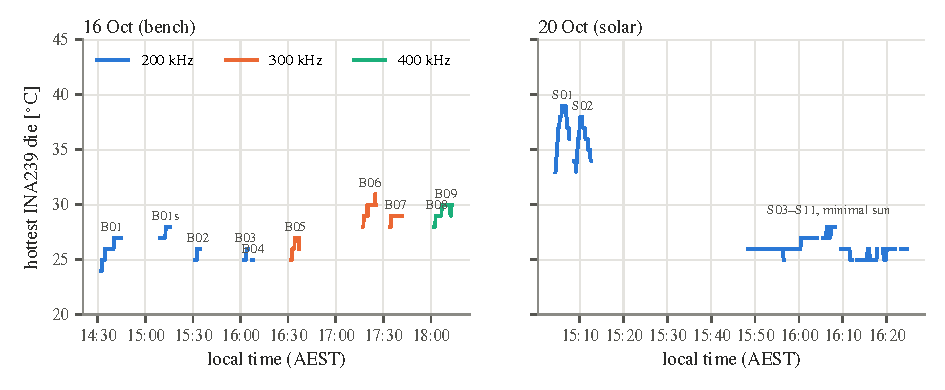
\includegraphics[width=\linewidth]{results/thermal}
  \caption[{Hottest INA239 die temperature in every test window}]{Hottest INA239 die temperature during every test window (10\,s maxima of the telemetry), coloured by switching frequency. The over-temperature trip is at 85\,$^\circ$C (INA die) and 80\,$^\circ$C (heatsink, Pi-side E-stop).}
  \label{fig:thermal}
\end{figure}
\begin{figure}[htbp]
  \centering
  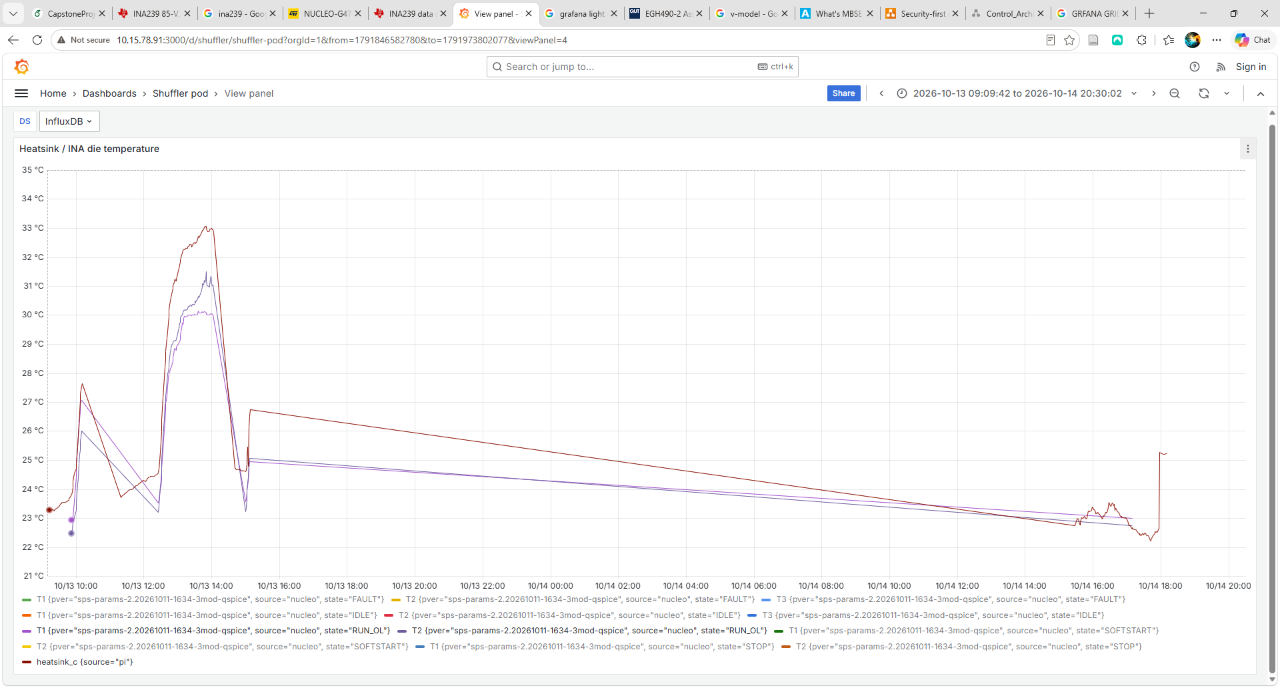
\includegraphics[width=0.7\linewidth]{misc/thermal_100k}
  \caption{Grafana capture of the 100\,kHz open-loop exploration on 13--14 Oct, which ran but behaved erratically.}
\end{figure}
\begin{figure}[htbp]
  \centering
  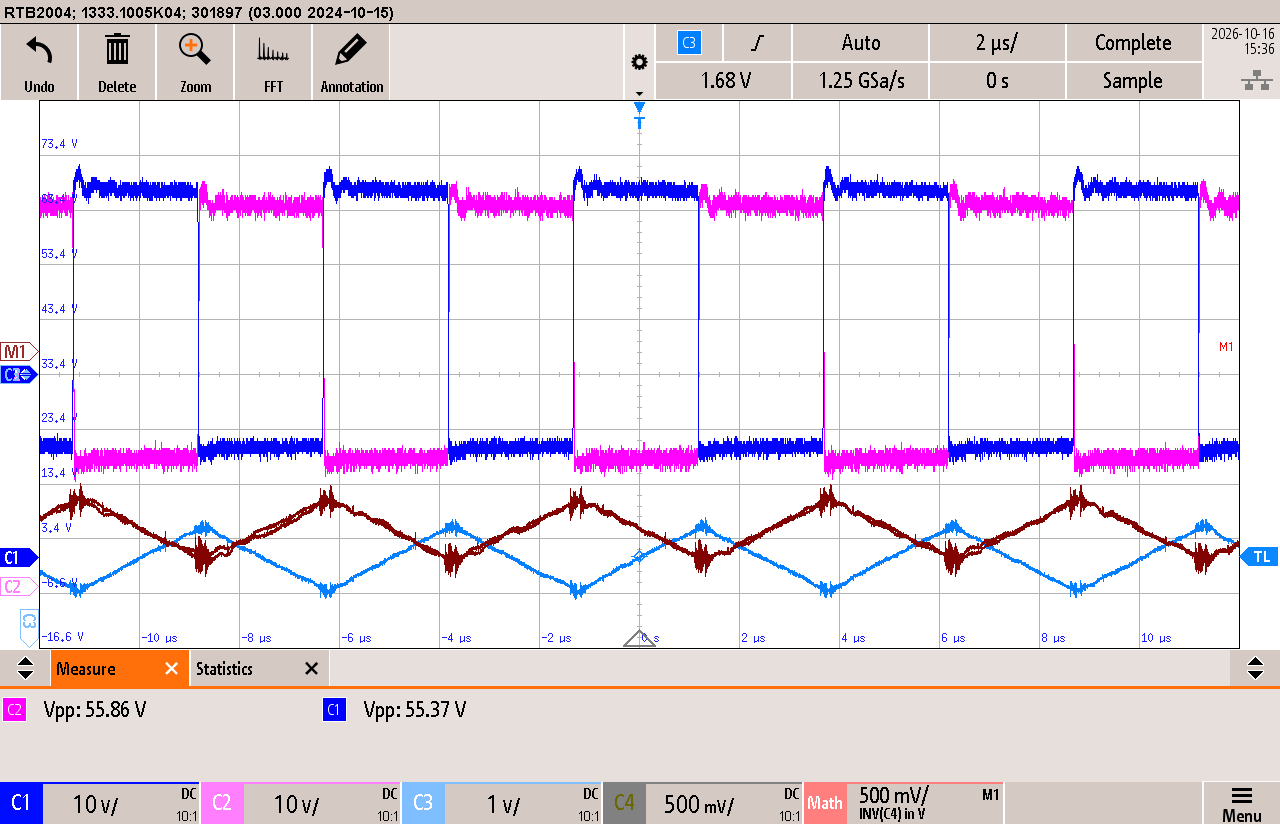
\includegraphics[width=0.32\linewidth]{misc/scope_200k}\hfill
  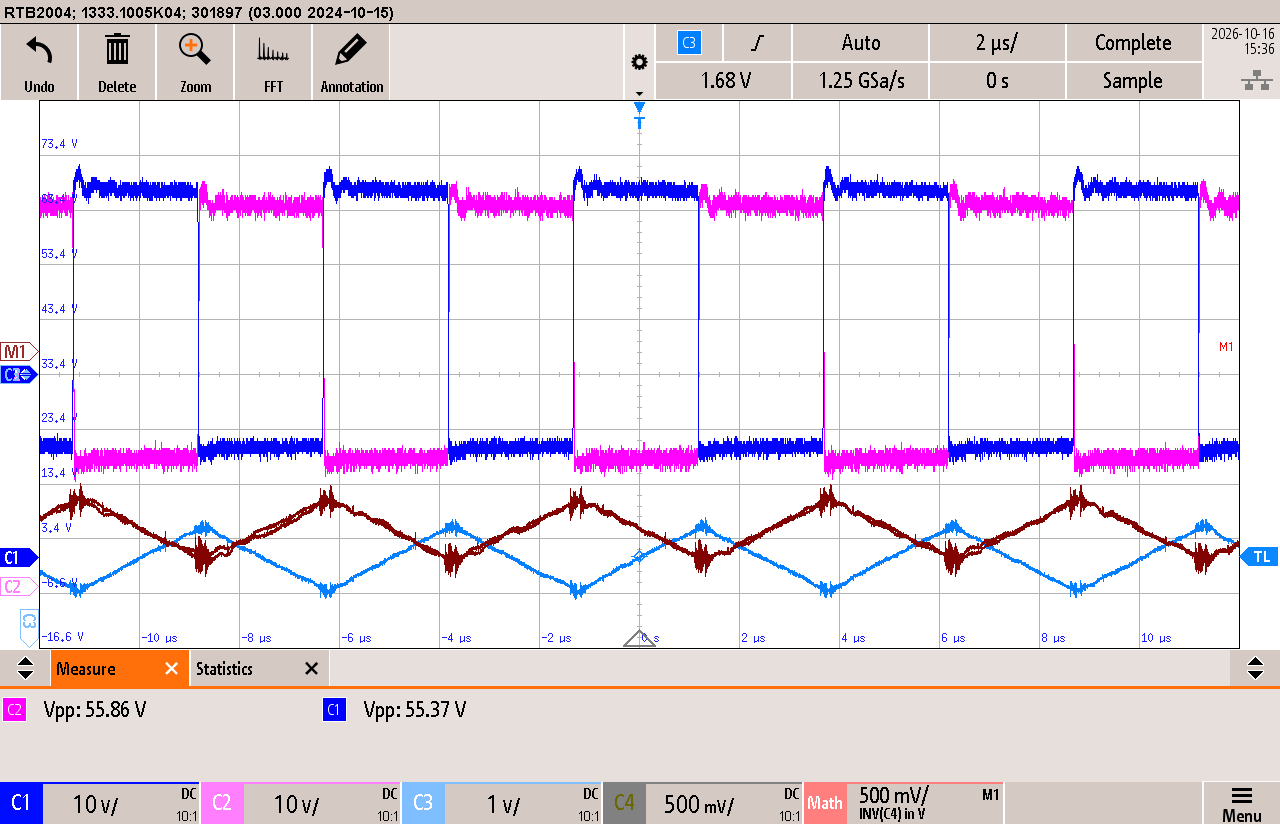
\includegraphics[width=0.32\linewidth]{misc/scope_300k}\hfill
  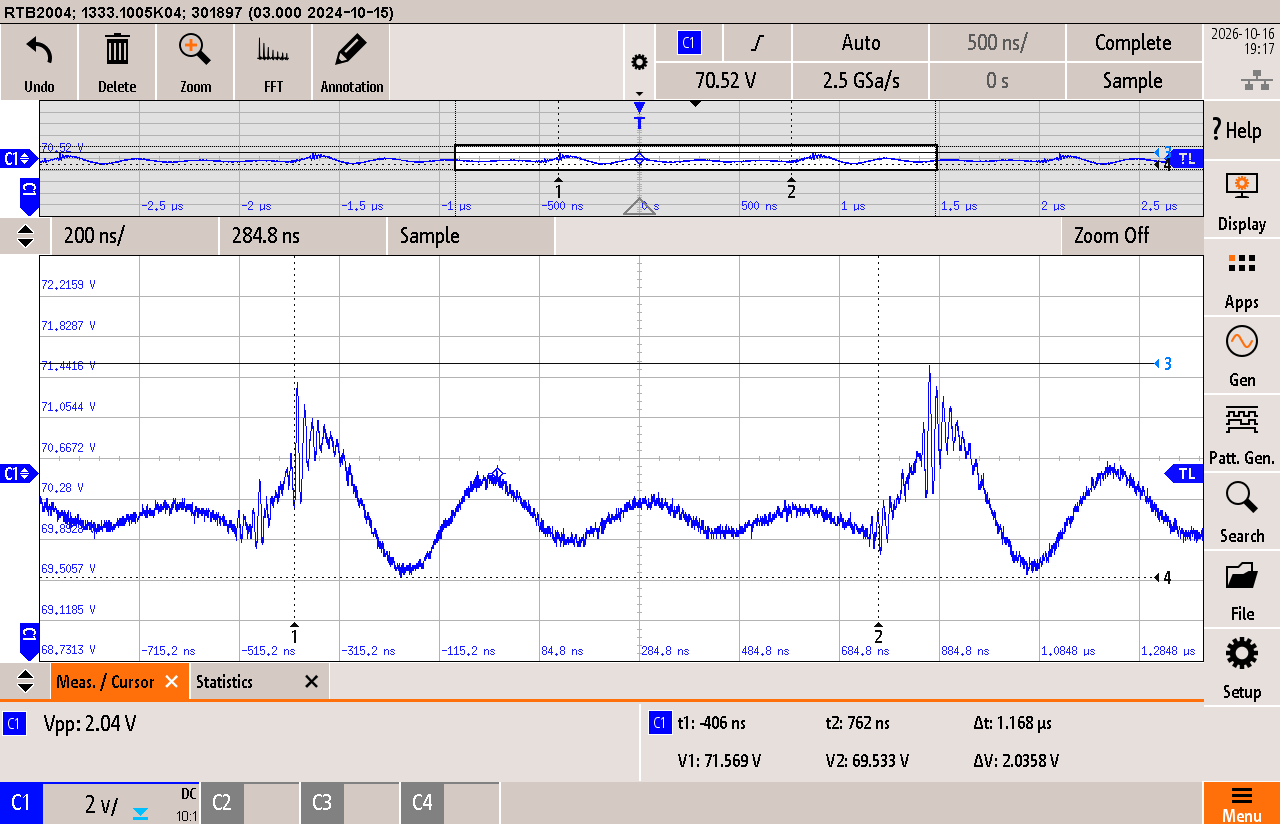
\includegraphics[width=0.32\linewidth]{misc/scope_400k}
  \caption{Oscilloscope captures of the switch-node waveforms at 200, 300 and 400\,kHz (dead time and 180$^\circ$ interleave check).}
  \label{fig:scope}
\end{figure}

\section{The Journey}
\label{app:journey}
\begin{figure}[htbp]
  \centering
  \begin{subfigure}[t]{0.32\linewidth}\centering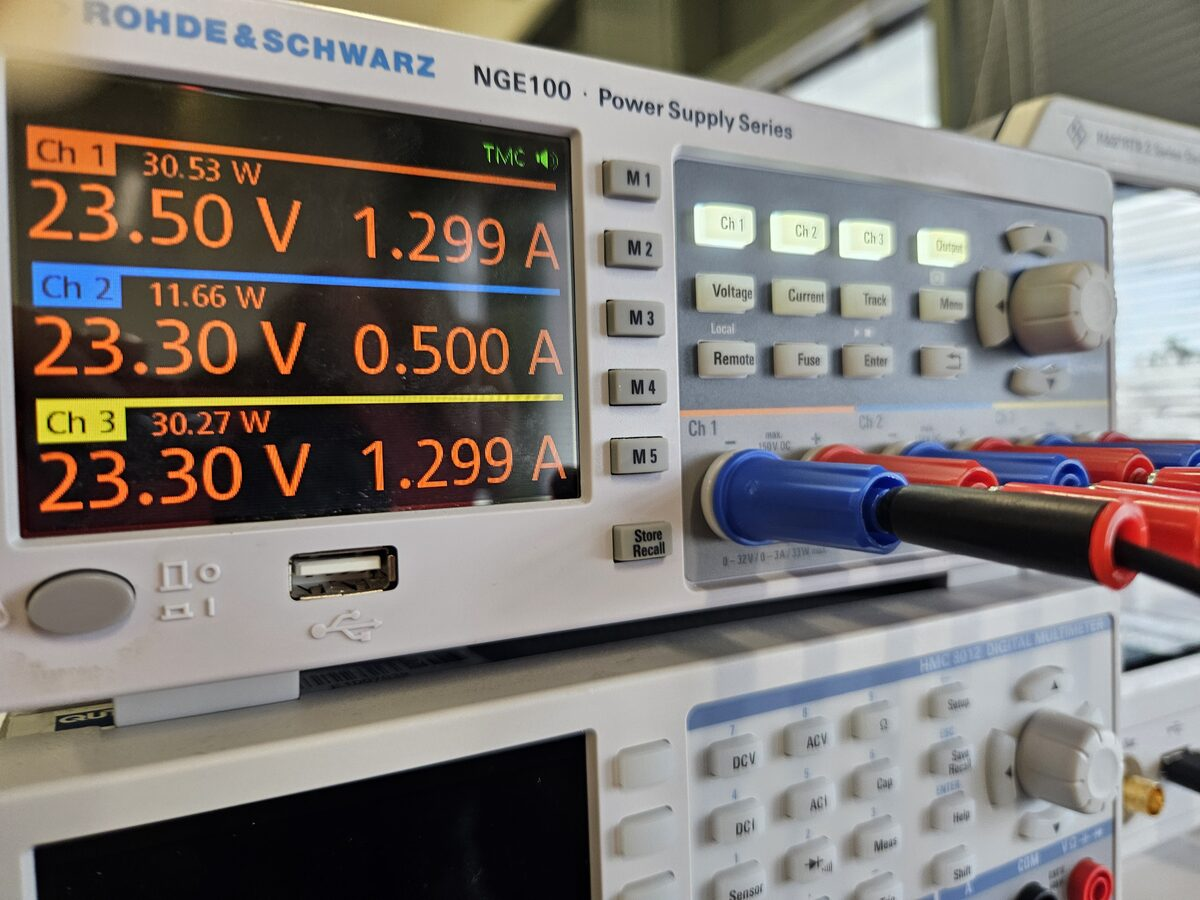
\includegraphics[width=\linewidth,height=3.4cm,keepaspectratio]{20261016_143219}\caption{NGE103 PSU: 23.30\,V / 1.299\,A, 23.30\,V / 0.500\,A, 23.30\,V / 1.299\,A.}\end{subfigure}\hfill
  \begin{subfigure}[t]{0.32\linewidth}\centering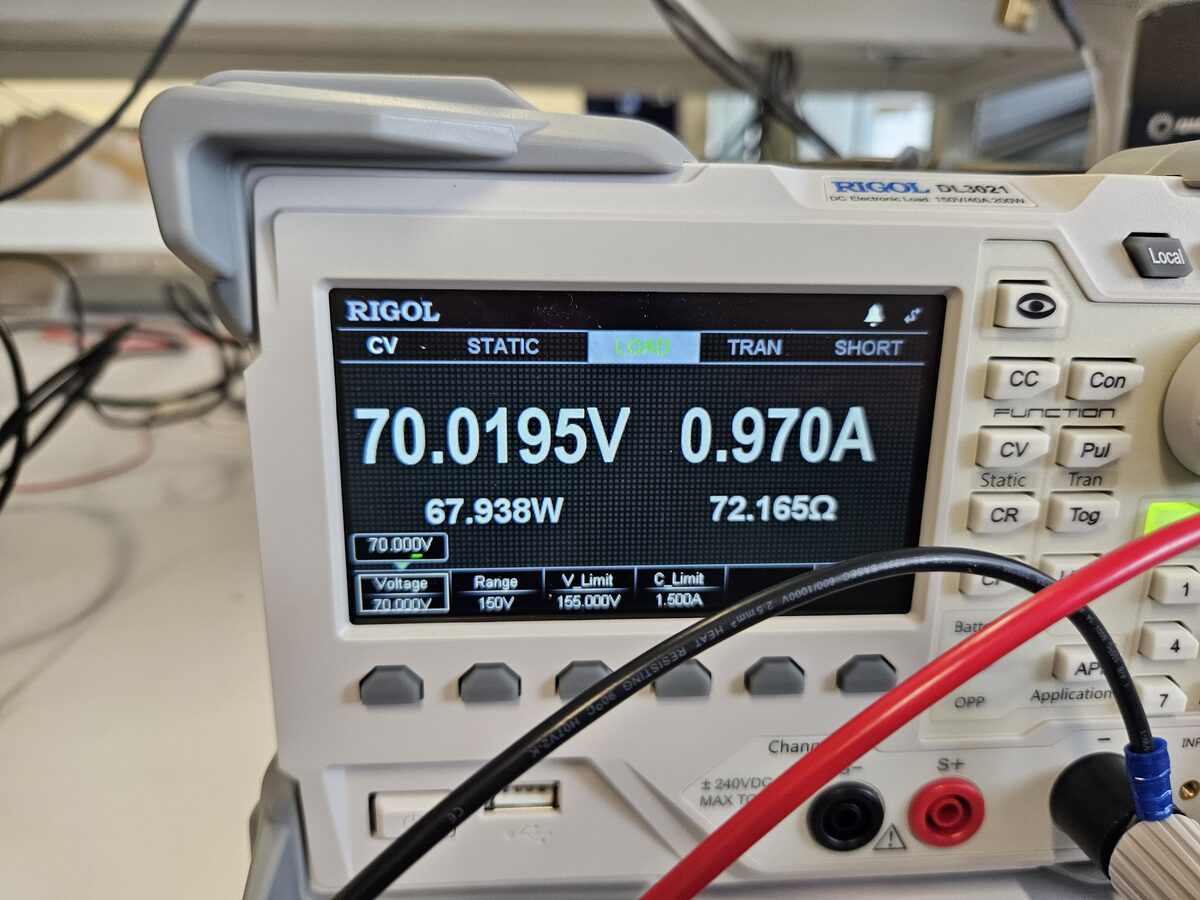
\includegraphics[width=\linewidth,height=3.4cm,keepaspectratio]{20261016_143227}\caption{DL3021 e-load in CV: 70.02\,V, 0.970\,A, 67.9\,W.}\end{subfigure}\hfill
  \begin{subfigure}[t]{0.32\linewidth}\centering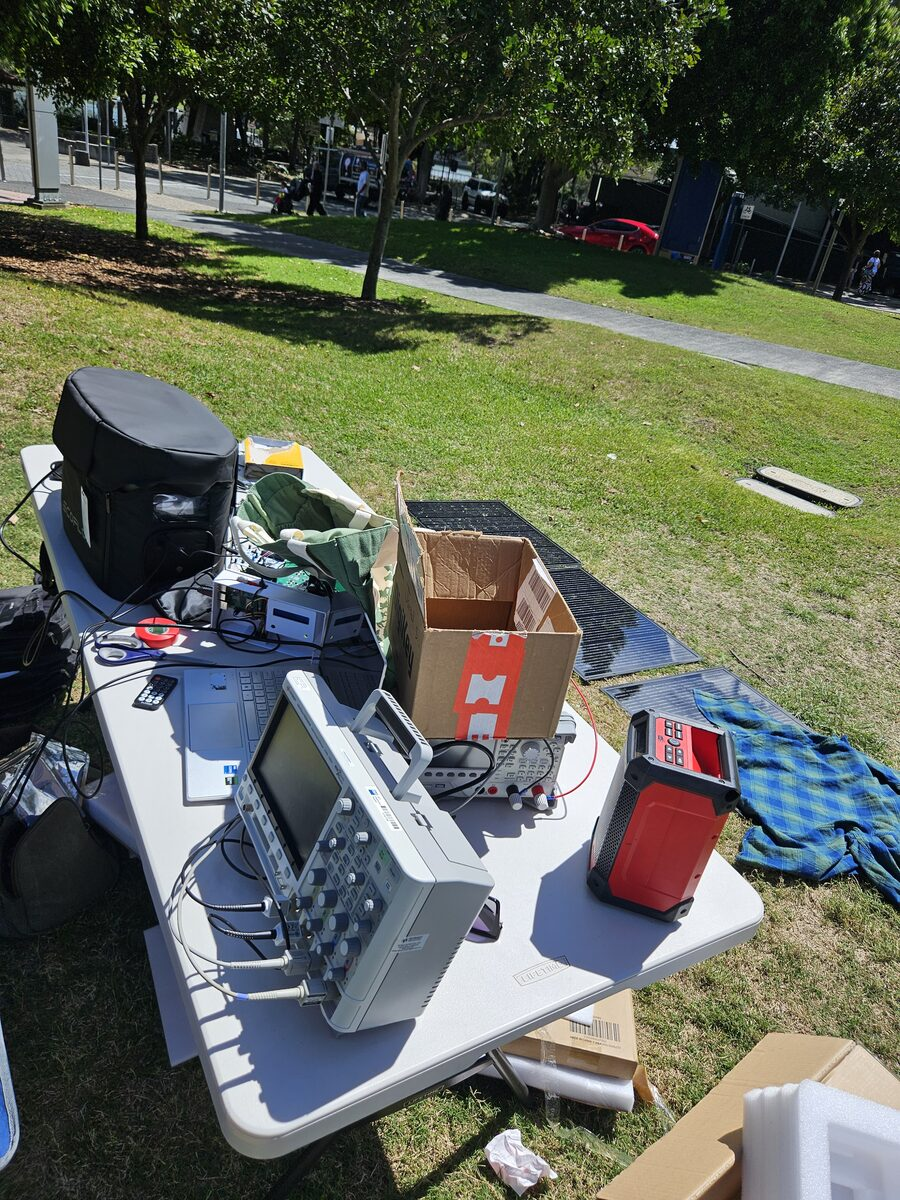
\includegraphics[width=\linewidth,height=3.4cm,keepaspectratio]{20261020_132132}\caption{Carpark string on 20 Oct 2026.}\end{subfigure}
  \caption[{Photographs of the two set-ups}]{Photographs of the two set-ups (more in \cref{app:journey}).}
  \label{fig:setupphotos}
\end{figure}
\newcommand{\ph}[2]{\begin{subfigure}[t]{0.32\linewidth}\centering\includegraphics[width=\linewidth,height=4.6cm,keepaspectratio]{#1}\caption{#2}\end{subfigure}}
\begin{figure}[htbp]
  \centering
  \ph{20260828_075344}{Aug: first proto-board with the Nucleo.}\hfill
  \ph{20260925_000522}{Sep: the Version 0 PCB arrives.}\hfill
  \ph{20261004_141445}{Oct 4: reflow in the PCB oven.}\\[3pt]
  \ph{20261004_162523}{Oct 4: assembled board with the Nucleo.}\hfill
  \ph{20261004_162616}{Oct 4: the hardware teammate with the board.}\hfill
  \ph{20261006_102236}{Oct 6: heatsink.}\\[3pt]
  \ph{20261007_081025}{Oct 7: enclosure work.}\hfill
  \ph{20261011_101108}{Oct 11: pod with the Pi, LCD and IR receiver.}\hfill
  \ph{20261014_100557}{Oct 14: heatsink mounted, thermal paste.}
  \caption{Build photographs (1 of 2).}
\end{figure}
\begin{figure}[htbp]
  \centering
  \ph{20261014_164518}{Oct 14: U10, the top INA239 behind the reversed isolator.}\hfill
  \ph{20261014_212624}{Oct 14: ERUC23 coupled inductor rework.}\hfill
  \ph{20261012_180815}{Oct 12: first bench runs.}\\[3pt]
  \ph{20261016_143209}{Oct 16: pod LCD during the bench test.}\hfill
  \ph{20261016_153331}{Oct 16: Grafana live during closed loop.}\hfill
  \ph{IMG-20261014}{Oct 14: late-night bring-up.}\\[3pt]
  \ph{20261020_131748}{Oct 20: carpark set-up.}\hfill
  \ph{20261020_131809}{Oct 20: it works in the sun.}\hfill
  \ph{20261020_132132}{Oct 20: the string.}
  \caption[{Build and test photographs (2 of 2)}]{Build and test photographs (2 of 2). Videos of the bench runs are in the project repository.}
\end{figure}


\end{document}
